% created on 12/05/2020
% @author : ebazan

\chapter{Color Texture Analysis Based on Spectral Decomposition}\label{ch:complex_spectral_image_decomposition}
\section*{Résumé}
\noindent Dans ce chapitre, nous présentons la décomposition spectrale d'une image couleur utilisant le filtre de Gabor. Nous utilisons la théorie des fonctions de Gabor développée au chapitre \ref{ch:spectral_image_decomposition} pour extraire les caractéristiques de texture locale d'une image en couleur. La stratégie principale consiste à transformer l'image d'entrée d'un espace couleur réel à trois canaux en une représentation couleur complexe à deux canaux. Ensuite, nous utilisons une banque de filtres Gabor sur chaque canal de l'image pour extraire les informations de texture générées par les variations de couleur et d'illumination de l'image.

\section*{Abstract}
\noindent  In this chapter, we present the spectral decomposition of a color image employing the Gabor filter. We use the Gabor functions theory developed in chapter \ref{ch:spectral_image_decomposition} to extract local features of a texture color. The primary strategy involves transforming the input image from a three-channel real color space into a two-channel complex color representation. Then, we use a bank of Gabor filters on each channel of the image to extract the texture information generated by the variations of color and illumination in the image. 

\section{Introduction}

Gabor filters have long been used for analyzing textures and extracting corresponding image features. Its adaptability and customization, depending on the application and the relationship with the human visual system  \citep{Daugman:JOSA:1985a}, have made this technique one of the most relevant for analyzing textures in an image. 

The use of Gabor filters for image texture analysis is highly dependent on the final application. Some of the most recognized works in the literature date back to the late 90s, where this technique was a hot research topic for image texture analysis. However, regarding the works present in the literature, we can separate the methods taking into account the nature of the extracted features. The first group uses Gabor filters to extract a global texture descriptor (Gabor signature). Generally, this strategy is suitable for applications where the images contain homogeneous textures, and it is sought to make the classification of images or an image retrieval system based on the content, as we can see in chapter \ref{ch:similarity_measures}. The second group is characterized by using Gabor filters to obtain local texture features present in an image. Such a strategy is suitable for image segmentation tasks. In this chapter, we address the second case straightforwardly and comprehensively, delving into the spectral decomposition of color images to obtain texture features generated by the changes in illumination and (or) color.

We take advantage of the Gabor function's dual-domain (spatial and frequency) representation capability to create a bank of filters $G=\{g_{f, \theta}(x, y) \}$ and obtain the spectral decomposition of an input image $I(x, y)$ through the convolution operation of each of the filters such that 
\begin{equation}\label{eq:gabor_responses}
    r_{f, \theta}(x,y) = I(x, y) \ast g_{f, \theta}(x,y)
\end{equation}
represents the filter response at different central frequencies $f$ (scales) and orientations $\theta$. Given the complex form of Gabor filters Eq. \eqref{eq:gabor_function_2d_spacefreq_bank} defined in chapter \ref{ch:spectral_image_decomposition}, the filter response $r_{f,\theta}(x, y)$ has a real and an imaginary part, here denoted as $\RE{(\cdot)}$ and $\IM{(\cdot)}$, respectively.

The linear transformation of an image using Eq. \eqref{eq:gabor_responses}, produces considerable information about the image's textures. The efficient manipulation of this information is the basis for extracting appropriate (local or global) texture features. Although the image's convolution by a filter bank is a common denominator in techniques based on signal processing, in the literature, we find various options to create more separable texture features (see Fig. \ref{fig:general_pipeline_gabor_feature_extraction}). In general, these methods differ in the type of output they use to measure the image's textural information and the post-processing techniques to refine the Gabor responses. Among the possible Gabor filter responses to measure the texture information, some of the most used in the literature are

\begin{enumerate}
    \item The amplitude of the response (magnitude or Gabor energy) \citep{Bovik.Clark.ea:TPAMI:1990}.
        \begin{equation}\label{eq:gabor_magnitude}
            |r_{f, \theta}(x,y)| = \sqrt{\RE{(r_{f, \theta}(x, y))}^2 + \IM{(r_{f, \theta}(x, y))}^2}
        \end{equation}
    \item The phase of the response \citep{Palm.Lehmann:MGV:2002}.
    \begin{equation}\label{eq:gabor_phase}
            \arg(r_{f, \theta}(x,y)) = \arctan2{\left(\frac{\IM{(r_{f, \theta}(x, y))}}{\RE{(r_{f, \theta}(x, y))}}\right)}
        \end{equation}
    \item The real component of the response \citep{Jain.Farrokhnia:IJPR:1991}.
    \begin{equation}\label{eq:gabor_real_part}
            \RE{(r_{f, \theta}(x, y))}
        \end{equation}
    \item The square amplitude of the response (Gabor local power spectrum) \citep{Grigorescu.Petkov.ea:TIP:2002}.
    \begin{equation}\label{eq:gabor_power}
            |r_{f, \theta}(x,y)|^2 = \RE{(r_{f, \theta}(x, y))}^2 + \IM{(r_{f, \theta}(x, y))}^2
        \end{equation}
\end{enumerate}
while the most common post-processing techniques for the filter outputs consist of a non-linear transformation followed by smoothing using a rectangular or Gaussian window \citep{Randen.Husoy:TPAMI:1999}, \citep{Clausi.EdJernigan:JPR:2000}. The application of non-linearity favors the activation of the textured areas in the images, while the smoothing favors the location of the energy obtained with the filter, avoiding the loss of information from the natural contours of the image. Figure \ref{fig:general_pipeline_gabor_feature_extraction} illustrates the stages (boxes with continuous black lining) and the input/outputs (boxes with black dotted lining) of the scheme mentioned above, referring to the extraction of Gabor-based texture features. 

\begin{figure}[!ht]
	\centering
	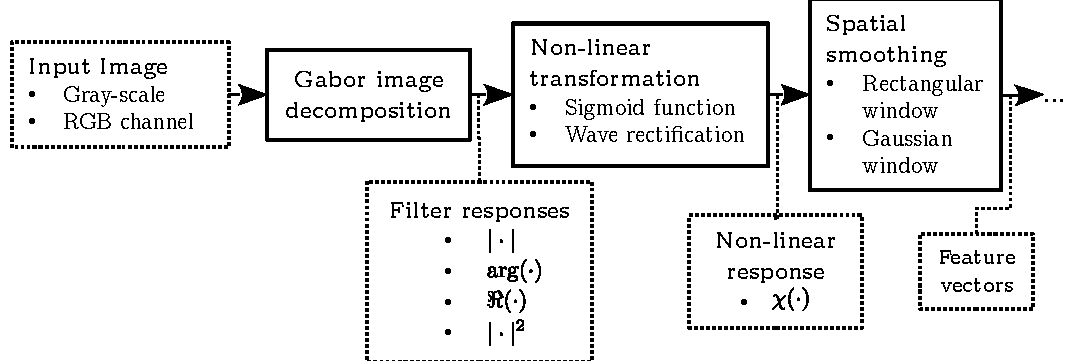
\includegraphics[width=\textwidth]{general_pipeline_gabor_feature_extraction}
	\caption{Pipeline of classic techniques for extraction of texture features using the Gabor filters. }\label{fig:general_pipeline_gabor_feature_extraction}
\end{figure}


\subsection{Texture features for color images}
Most of the research work on texture has been done using gray-scale images and with homogeneous textures; see for example \citep{Jain.Farrokhnia:IJPR:1991}, \citep{ChengjunLiu.Wechsler:NN:2003}, \citep{Liu.Koga.ea:ICDAR:2005}, \citep{Al-Kadi:arXiv:2017}. Consequently, the simplest way to obtain texture features from color images is to transform them into a gray-scale image. This strategy favors the acceleration of feature calculation because we work with scalar values instead of vectors. However, despite the good results in images with homogeneous gray-scale textures, reducing channels for a natural-color image with non-homogeneous textures does not ensure the generation of representative texture features. This outcome is primarily because the non-homogeneous textures in a color image are generated by luminance variations and variations in chromaticity. Moreover, the real-world scenes are in color and contain non-homogeneous textures.  For example, in the case of a texture image in the RGB color space, which its gray-scale transformation represents the levels of red, green, and blue \citep{Artusi.Banterle.ea:Book:2016} as
%L = 0.2126 R + 0.7152 G + 0.00722 B
\begin{equation}\label{eq:color2gray_formula}
    L = 0.299 R + 0.587 G + 0.114 B    
\end{equation} 
if the image contains isoluminant colors (colors with the same luminance value), the transformation $L$ leads to a minimization or lost, in the worst case, of textures generated by the color changes.
%\textit{Idea to develope:} Illustrate the effect of compute unichrome features in the gray-scale and the RGB space for a color image.

% for a colored real-world image containing non-homogeneous textures. 
% Although there is some texture information in the color input image,

Notwithstanding, we find a large number of methods that propose the characterization of textures in color images. Such methods generally use two strategies for the analysis of color textures \citep{Maenpaa.Pietikainen:PR:2004}, \citep{Qazi.Alata.ea:PR:2011}:

\begin{itemize}
	\item process color and texture information separately
	\item process color and texture as a joint phenomenon
\end{itemize} 

The first category methods assume that the spatial variations that form textures and color distributions of the image are independent cues (see for example \citep{Permuter.Francos.ea:PR:2006}). We differ from this point of view, and we consider that color and texture information in an image is a joint phenomenon based on the idea that textural segmentation occurs based on the distribution of simple properties of texture elements, for example, the brightness, color, size, and the slopes of contours and other elemental descriptors of a texture \citep{Werner.Chalupa:Book:2004}.
 
In this regard, there are various techniques to joint color and texture information to characterize natural color textures. A popular option is to get unichromatic texture features from each color channel of the image using, for example, Gabor filters. Taking the RGB color space as a reference, the filter responses represent the texture features of each primary color red, green, and blue independently, i.e., in principle, this strategy does not involve the correlation between RGB band colors. This strategy might be corrected using the opponent color model based on the human color vision theory \citep{Jain.Healey:TIP:1998}. In such a case, each unichromatic feature vector (RGB-feature) is multiplied and normalized by the feature vector of its opponent color to include the correlation between color channels \citep{Palm.Keysers.ea:JCIS:2000}. This method manages to gather the information of color and texture under a frame of human color perception. However, the normalization and multiplication of the unichromatic texture feature vectors imply extra post-processing steps in the features extraction pipeline.  

One way to avoid the post-processing stage after the image Gabor decomposition is to first transform the color image in a color space that handles the coupling between the color channels rather than separating them as individual components of the color space. The quaternion framework \citep{Sangwine.Ell:VISP:2000} provides this possibility of coupled color representation. It encodes the color value of each pixel in a pure quaternion, where the real component is set to zero, and the three imaginary components represent the color band, such as $I(x, y) = R (x, y) \mathsf{i} + G (x, y) \mathsf{j} + B (x, y) \mathsf{k}$. This 3-component vector representation yields a system with well-defined mathematical operations, such as Quaternion Fourier Transform, that makes the Gabor image decomposition possible through the Quaternion Gabor Filters (QBF) \citep{Subakan.Vemuri:EMMCVPR:2009}. However, when using quaternion values, the non-existing commutativity must be considered; the QGF does not support any physic interpretation of what is measured. 

Another alternative to this problem is to represent the image in one of the two-channel color spaces, previously defined in chapter \ref{ch:color_texure_representations}, where one channel contains the luminance information and the other the chrominance information of the image. We can obtain such a representation from the non-linear color spaces like LAB or LUV and HSV or HSL perceptual color spaces. The representation in the form of luminance-chrominance has the characteristic of concentrating the color information in a complex channel, which is compatible with the multispectral Gabor decomposition. In both cases, the choice of a pertinent color space for the texture's characterization is necessary \citep{Qazi.Alata.ea:PR:2011}.

The methodology we present in this chapter mainly follows the stages shown in the diagram of figure \ref{fig:general_pipeline_gabor_feature_extraction}. We introduce some modifications to exploit the color and texture information in the same framework. The modifications proposed to this scheme are transforming the input image from the RGB color space to one of the luminance-chrominance spaces (or complex two-channel color spaces) described in chapter \ref{ch:color_texure_representations}. Then, the non-linear transformation was replaced by a morphological opening followed by an adaptive Gaussian smoothing to highlight the amplitude of the filter responses. Under this configuration, we obtain a spectral decomposition of the image that considers the textures generated by changes in lighting and those generated by color changes. Figure \ref{fig:proposed_pipeline_gabor_feature_extraction} shows the stages we perform for the extraction of local features.

Later in the chapter, we apply the Gabor feature space for the segmentation of natural color images. 

\begin{figure}[!ht]
	\centering
	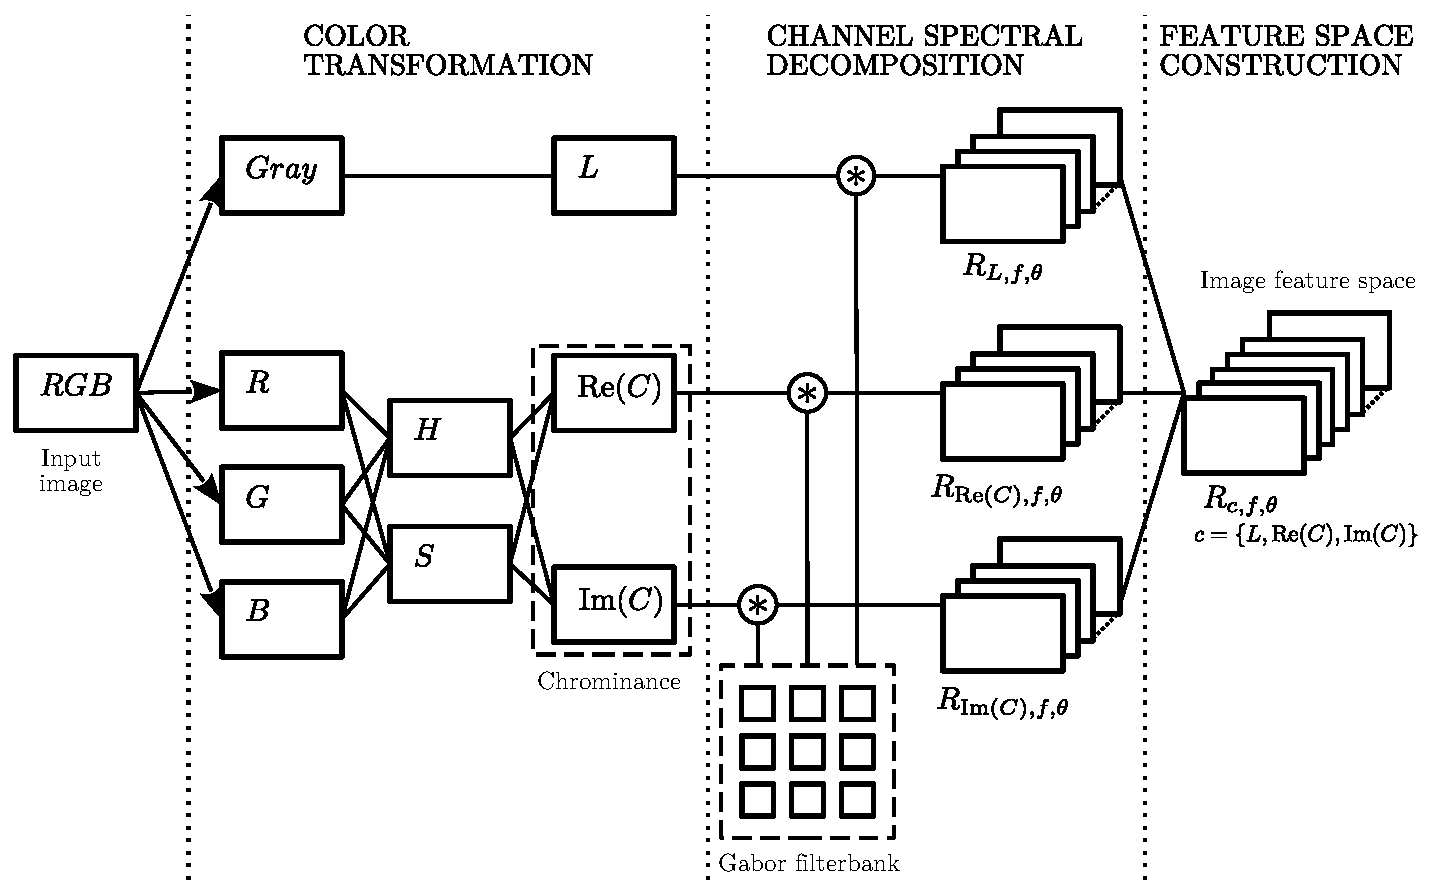
\includegraphics[width=\textwidth]{gabor_color_feature_extraction_diagram}
	\caption{The proposed methodology for the computation of Gabor features in color images.}\label{fig:proposed_pipeline_gabor_feature_extraction}
\end{figure}

%\section{Spectral decomposition of color images}
\section{Gabor Filter-based Texture Feature Space}

\subsection{Color Image Transformation}
The first stage in creating the feature space is transforming the input image from the RGB color space to the two-channel luminance-chrominance space. The representation in two channels, one real and the other complex, of a color image, allows us to separate the intervention of luminance and colors in the generation of textures in an image. To help visualize such a joint phenomenon, we create a synthetic image that reflects the complexity of natural color images.

\subsubsection{Synthetic image description}
The synthetic image we create contains seven different regions with spatial variations (textures) generated by alternating various colors at different frequencies. Each tile of the image is perceived as a whole; this is perceptually a constant region. The colors alternate along different directions in the chrominance phase (Fig. \ref{fig:color_complex_plane}). The last image region has two frequency components.

We generate the input image with the sign function of a 2-d sinusoidal signal multiplied by the color values of each region in the RGB color space such that
\begin{gather}
	I(x, y) = sgn( \sin 2 \pi (f_x x_r + f_y y_r)) \cdot [R, G, B]\label{eq:2D_squared_signal}\\
	x_r = x \cos\theta + y \sin\theta \nonumber \\
    y_r = -x \sin\theta + y \cos\theta \nonumber  
\end{gather}

We control the image texture by varying the frequencies $f_{x}, f_{y}$ and the orientation angle $\theta$ of the coordinate plane $(x, y)$, where $\theta=0^\circ$ means vertical variations and $\theta=90^\circ$ horizontal variations. The proposed image has a size of $320\times1400$ pixels. The seven characteristic regions of the image are spread over $1400$ pixels wide, so each region is about $320\times200$ pixels, that is, the color/texture distribution in the image changes every 200 pixels (on the $x$-axis). The following expressions define the image spatial variations.  
\begin{gather}
	f_{x} = 
	\begin{cases} 
      0    & 0\leq x\leq 200  \\
      1/64 & 201\leq x\leq 400  \\
      1/32 & 401\leq x\leq 600  \\
      1/16 & 601\leq x\leq 800  \\
      1/8  & 801\leq x\leq 1000  \\
      1/4  & 1001\leq x\leq 1200 \\   
      1/8  & 1201\leq x\leq 1400 \\ 
   	 \end{cases} \nonumber ; \quad
   	 f_{y} = \begin{cases} 
      0    & 0\leq x\leq 200  \\
      0    & 201\leq x\leq 400  \\
      0    & 401\leq x\leq 600  \\
      0    & 601\leq x\leq 800  \\
      0    & 801\leq x\leq 1000  \\
      0    & 1001\leq x\leq 1200 \\  
      1/32 & 1201\leq x\leq 1400 \\ 
   	 \end{cases} \nonumber  
\end{gather}

For comprehension purposes, we use colors easily identified in the RGB space (primary colors) or in the HSV space (perceptual colors) to generate the image textures. Figure \ref{fig:synthetic_color_texture_image} depicts the resulting synthetic image. 

\begin{figure}[!ht]
    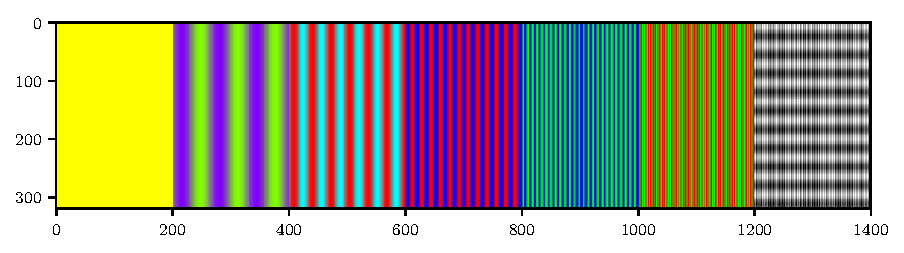
\includegraphics[width=\textwidth]{synthetic_image_color_texture}
\caption{Synthetic color textured image.}\label{fig:synthetic_color_texture_image}
\end{figure}

The 2-d sinusoidal modulations generates textures in the image at a different and well known frequencies. These modulations change the colors of the regions generating a texture of oriented lines. The regions of the synthetic image have the following color and texture characteristics.

\paragraph{Region 1. Textureless zone:}
This region does not contain spatial variations, i.e., it has only a solid color. The color of the region is yellow (arbitrarily chosen).

\paragraph{Region 2. Lowest frequency textured zone with colors on the imaginary plane:}
This region is described by the vertical texture generated by variations between purple and green lime. Such colors are found in the imaginary axis of the chrominance plane. The colors in this region change every 64 pixels (along the $x$-axis).

\paragraph{Region 3. Textured zone with colors on the real plane:}
This region contains a vertical texture generated by the variations between red and cyan. Such colors are found in the real axis of the chrominance plane. The colors in this region change every 32 pixels (along the $x$-axis).

\paragraph{Region 4. Textured zone with two primary colors:}
The horizontal texture of this region is generated by the variations between red and blue. The colors in this region change every 16 pixels (along the $x$-axis). 

\paragraph{Region 5. Textured zone with two primary colors:}
The horizontal texture of this region is generated by the variations between blue and green. The colors in this region change every 8 pixels (along the $x$-axis). 

\paragraph{Region 6. Textured zone with two primary colors:}
The horizontal texture of this region is generated by the variations between green and red. The colors change every 4 pixels (along the $x$-axis).

\paragraph{Region 7. Colorless mixed textures zone:}
This region contains two textures, both of them formed by the variations between black and white, i.e., there is no color information. Moreover, the textures change in frequency and orientation; the pixes of the horizontal texture change of color every 4 pixels along the $x$-axis (highest frequency), while the pixel values of the vertical texture changes every 16 pixels along the $y$-axis (same frequency as region 4).

We summarize the colors and frequency of each zone in Table \ref{tab:synthetic_image_components}. In the table, we expose the $RGB$ and $HSV$ values of the texture-forming colors as well as the frequency and orientation of each section.


\begin{table}[!h]
\resizebox{\textwidth}{!}{%
\begin{tabular}{c|ccccccc}
                    & \multicolumn{7}{c}{\textbf{Region}}                                                                                                                                                                          \\ \hline
\textbf{}           & 1                  & 2                   & 3                   & 4                   & 5                   & 6                   & 7                                                              \\ \hline
\textbf{Color 1}    &                    &                     &                     &                     &                     &                     &                                                                \\
\textit{Name}       & Yellow             & Purple              & Red                 & Red                 & Blue                & Green               & Black                                                          \\
\textit{RGB values} & {[}255, 255, 0{]}  & {[}128, 0, 255{]}   & {[}255, 0, 0{]}     & {[}255, 0, 0{]}     & {[}0, 0, 255{]}     & {[}0, 255, 0{]}     & {[}0, 0, 0{]}                                                  \\
\textit{HSV values} & {[}60, 100, 100{]} & {[}270, 100, 100{]} & {[}0, 100, 100{]}   & {[}0, 100, 100{]}   & {[}240, 100, 100{]} & {[}120, 100, 100{]} & {[}0, 0, 0{]}                                                  \\ \hline
\textbf{Color 2}    &                    &                     &                     &                     &                     &                     &                                                                \\
\textit{Name}       & -                  & Green lime          & Cyan                & Blue                & Green               & Red                 & White                                                          \\
\textit{RGB values} & -                  & {[}128, 255, 0{]}   & {[}0, 255, 255{]}   & {[}0, 0, 255{]}     & {[}0, 255, 0{]}     & {[}255, 0, 0{]}     & {[}255, 255, 255{]}                                            \\
\textit{HSV values} & -                  & {[}90, 100, 100{]}  & {[}180, 100, 100{]} & {[}240, 100, 100{]} & {[}120, 100, 100{]} & {[}0, 100, 100{]}   & {[}0, 0, 100{]}                                                \\ \hline
\textbf{Texture}    &                    &                     &                     &                     &                     &                     &                                                                \\
\textit{Freq.}      & -                  & $1/64$              & $1/32$              & $1/16$              & $1/8$               & $1/4$               & \begin{tabular}[c]{@{}c@{}}$1/8$\\ $1/32$\end{tabular}         \\
\textit{Angle}      & -                  & $90^\circ$          & $90^\circ$          & $90^\circ$          & $90^\circ$          & $90^\circ$          & \begin{tabular}[c]{@{}c@{}}$0^\circ$\\ $90^\circ$\end{tabular}
\end{tabular}}
\caption{Specifications of the color and texture settings for each of the regions within the synthetic image.}\label{tab:synthetic_image_components}
\end{table}




%\begin{table}[h!]
%\resizebox{\textwidth}{!}{%
%\begin{tabular}{c|c|c|c|c|c|c|c|c|}
%\cline{2-9}
%\textbf{}                                & \multicolumn{6}{c|}{\textbf{Colors}}                                                                                                                                        & \multicolumn{2}{c|}{\multirow{2}{*}{\textbf{Texture}}} \\ \cline{2-7}
%                                         & \multicolumn{3}{c|}{\textbf{Color 1}}                                            & \multicolumn{3}{c|}{\textbf{Color 2}}                                                    & \multicolumn{2}{c|}{}                                  \\ \hline
%\multicolumn{1}{|c|}{\textbf{Zone}}      & \textbf{Name}          & \textbf{$RGB$ values}      & \textbf{$HSV$ values}      & \textbf{Name}          & \textbf{$RGB$ values}            & \textbf{$HSV$ values}        & \textbf{Freq.}             & \textbf{Angle}            \\ \hline
%\multicolumn{1}{|c|}{1}                  & Yellow                 & $[255,255,0]$              & $[60,100,100]$             & n/a                    & n/a                              & n/a                          & n/a                        & $90^\circ$                \\ \hline
%\multicolumn{1}{|c|}{2}                  & Purple                 & $[128, 0, 255]$            & $[270,100,100]$            & Green lime             & $[128, 255, 0]$                  & $[90,100,100]$               & $\frac{1}{64}$             & $90^\circ$                \\ \hline
%\multicolumn{1}{|c|}{3}                  & Red                    & $[255,0,0]$                & $[0,100,100]$              & Cyan                   & $[0,255,255]$                    & $[180,100,100]$              & $\frac{1}{32}$             & $90^\circ$                \\ \hline
%\multicolumn{1}{|c|}{4}                  & Red                    & $[255,0,0]$                & $[0,100,100]$              & Blue                   & $[0,0,255]$                      & $[240,100,100]$              & $\frac{1}{16}$             & $90^\circ$                \\ \hline
%\multicolumn{1}{|c|}{5}                  & Blue                   & $[0,0,255]$                & $[240,100,100]$            & Green                  & $[0,255,0]$                      & $[120,100,100]$              & $\frac{1}{8}$              & $90^\circ$                \\ \hline
%\multicolumn{1}{|c|}{6}                  & Green                  & $[0,255,0]$                & $[120,100,100]$            & Red                    & $[255,0,0]$                      & $[0,100,100]$                & $\frac{1}{4}$              & $90^\circ$                \\ \hline
%\multicolumn{1}{|c|}{\multirow{2}{*}{7}} & \multirow{2}{*}{Black} & \multirow{2}{*}{$[0,0,0]$} & \multirow{2}{*}{$[0,0,0]$} & \multirow{2}{*}{White} & \multirow{2}{*}{$[255,255,255]$} & \multirow{2}{*}{$[0,0,100]$} & $\frac{1}{4}$              & $90^\circ$                \\ \cline{8-9} 
%\multicolumn{1}{|c|}{}                   &                        &                            &                            &                        &                                  &                              & $\frac{1}{32}$             & $0^\circ$                 \\ \hline
%\end{tabular}}
%\caption{Specifications of color and texture of the areas of the synthetic study image.}\label{tab:synthetic_image_components}
%\end{table}

\subsubsection{Graphical display of the synthetic image color distribution}
The choice of texture-forming colors comes from the interest in visualizing the color spectrum of the image more graphically. The two-channel color spaces, described in chapter \ref{ch:color_texure_representations}, encode color information in a complex chrominance channel. Therefore, we can interpret the chrominance values as points within a complex plane (see Fig. \ref{fig:color_complex_plane}). In the case of LAB/LUV spaces, the values of chrominance are defined in Cartesian coordinates as 
\begin{equation}\label{eq:chrominance_lab2}
    C = A + \mathsf{i}B
\end{equation}
where channel A values represent the real axis coordinates, and channel B values represent the imaginary axis coordinates. 

HSV/HSL color spaces encode chrominance values as points in polar coordinates 
\begin{equation}\label{eq:chrominance_hsv2}
    C = S \mathsf{e}^{\mathsf{i}H}
\end{equation}
where channel H values are the angle expressed radians and channel S values are the distance from the origin to the color points.

Considering these two chrominance configurations, the one defined by hue and saturation provides a more straightforward geometric interpretation of chrominance. Originally hue is a cylindrical dimension representing the color tints in the chromatic circle as angles, while saturation, which represents the purity of color, places achromatic tints in the center of the circle and pure colors on the circular edge of the disk. In figure \ref{fig:color_complex_plane}, we show the synthetic image color distribution plot using the HS dimensions in the 2-d chrominance complex plane. The hue $H$ is expressed in degrees, and saturation $S$ is normalized between $0$ and $255$. This representation complements the description of our synthetic test image Fig. \ref{fig:synthetic_color_texture_image}, showing the variation between colors that generate textures. We can notice in the chroma circle of figure \ref{fig:color_complex_plane} the transition between the red-green-blue primary colors at $0^\circ$, $120^\circ$ and $240^\circ$ respectively; the transition between purple and lime green on the imaginary axis with a hue of $90^\circ$ and $270^\circ$ respectively; the transition between red at $0^\circ$ and cyan at $180^\circ$ passing through the real axis of the plane and finally; the yellow color with a hue value of $60^\circ$.

\begin{figure}[!ht]
	\centering
    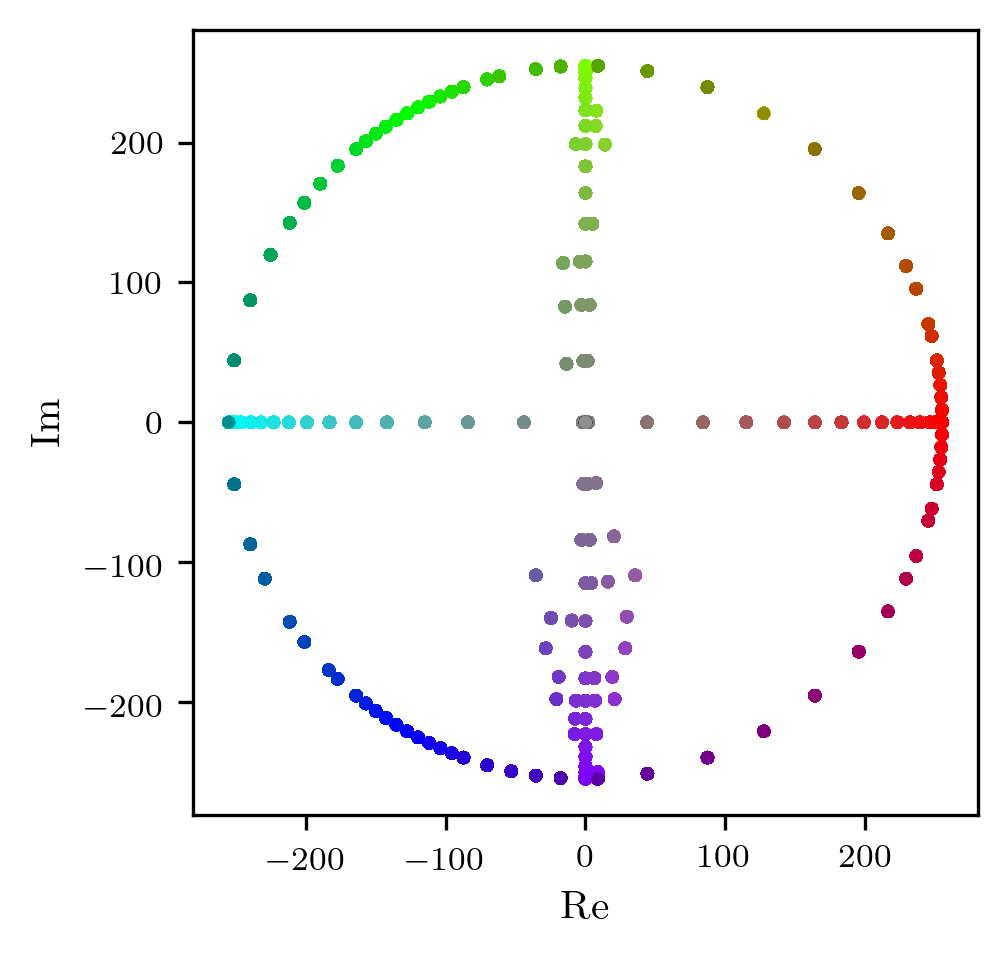
\includegraphics[width=0.8\textwidth]{color_complex_plane}
	\caption{Synthetic image chrominance distribution represented in the color complex plane.}\label{fig:color_complex_plane}
\end{figure}

Under this color space configuration, the colors of an image are represented in the complex chrominance plane. However, in this plane, the variations due to luminance information do not appear. The brightness of the colors is captured in the luminance channel. Depending on the color space that we use to build the two-channel color representation, we can obtain the luminance channel in different ways. In the LAB/LUV and HSL color spaces, the luminance channel is directly represented by the values of the $L$ dimension. In the HSV color space, we use the image transformation from RGB to gray-scale following the Eq. \eqref{eq:color2gray_formula} to obtain the luminance channel.

Figure \ref{fig:three_channel_decomposition} shows the three dimensions of the two-channel representation of the synthetic image ($L(x,y)$, $\RE(C(x,y))$, $\IM(C(x,y))$) in grayscale. In this representation, we use the HSV color space as a basis to obtain the luminance and chrominance values, so the $L$ channel is obtained with Eq. \eqref{eq:color2gray_formula} and the $C$ channel with Eq. \eqref{eq:chrominance_hsv2}. In figure \ref{fig:three_channel_decomposition}, we can see how the different regions show more or less important values depending on the channel in which they are. For example, the horizontal and vertical spatial variations of region 7 (between 1200 and 1400 column pixels) are only visible in the luminance channel $L(x,y)$ (see left image in \ref{fig:three_channel_decomposition}). We observe this same effect in the chrominance channels, for example, with the vertical textures of region 3. The spatial variations of this region are made up by the alternation of colors that live only in the real plane of chrominance (red and cyan), so the texture is only visible in channel $\RE(C(x,y))$ (see column pixels between 400 and 600 of the central image and the image to the right of subfigure \ref{fig:three_channel_decomposition}). 

We can also visualize the color variations and their influence on the generation of textures by plotting a horizontal line using a row of pixels' intensity values for each dimension of the two-channel space. In figure \ref{fig:horizontal_line_three_channel_decomposition}, we show the variations generated by changes in color and (or) lightness in a 1-d plot. Taking the area without texture (region 1), the horizontal line between pixels 0 and 200 remains constant in all three channels due to the absence of texture. However, in region 2, which corresponds to the low-frequency texture formed by the colors at $90^\circ$ and $270^\circ$ in the chroma circle, we see that variations are only present in the imaginary channel of chrominance $\IM(C(x,y))$. In regions 4, 5, and 6, since the texture-forming colors are two of the three primary colors (red, green, blue), the variations are visible in all three luminance-chrominance representation channels. Finally, in the last region (colorless mixed textures zone), we can see that the variations are only present in the channel that describes the luminance $L(x,y)$.

\begin{figure}[!ht]
\centering
    \subcaptionbox{\label{fig:synthetic_image_three_channel_decomposition}}{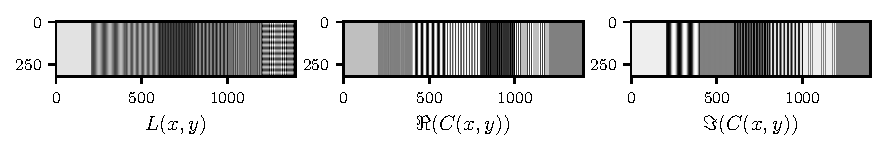
\includegraphics[width=\textwidth]{synthetic_image_three_channel_decomposition}}
    \subcaptionbox{\label{fig:horizontal_line_three_channel_decomposition}}{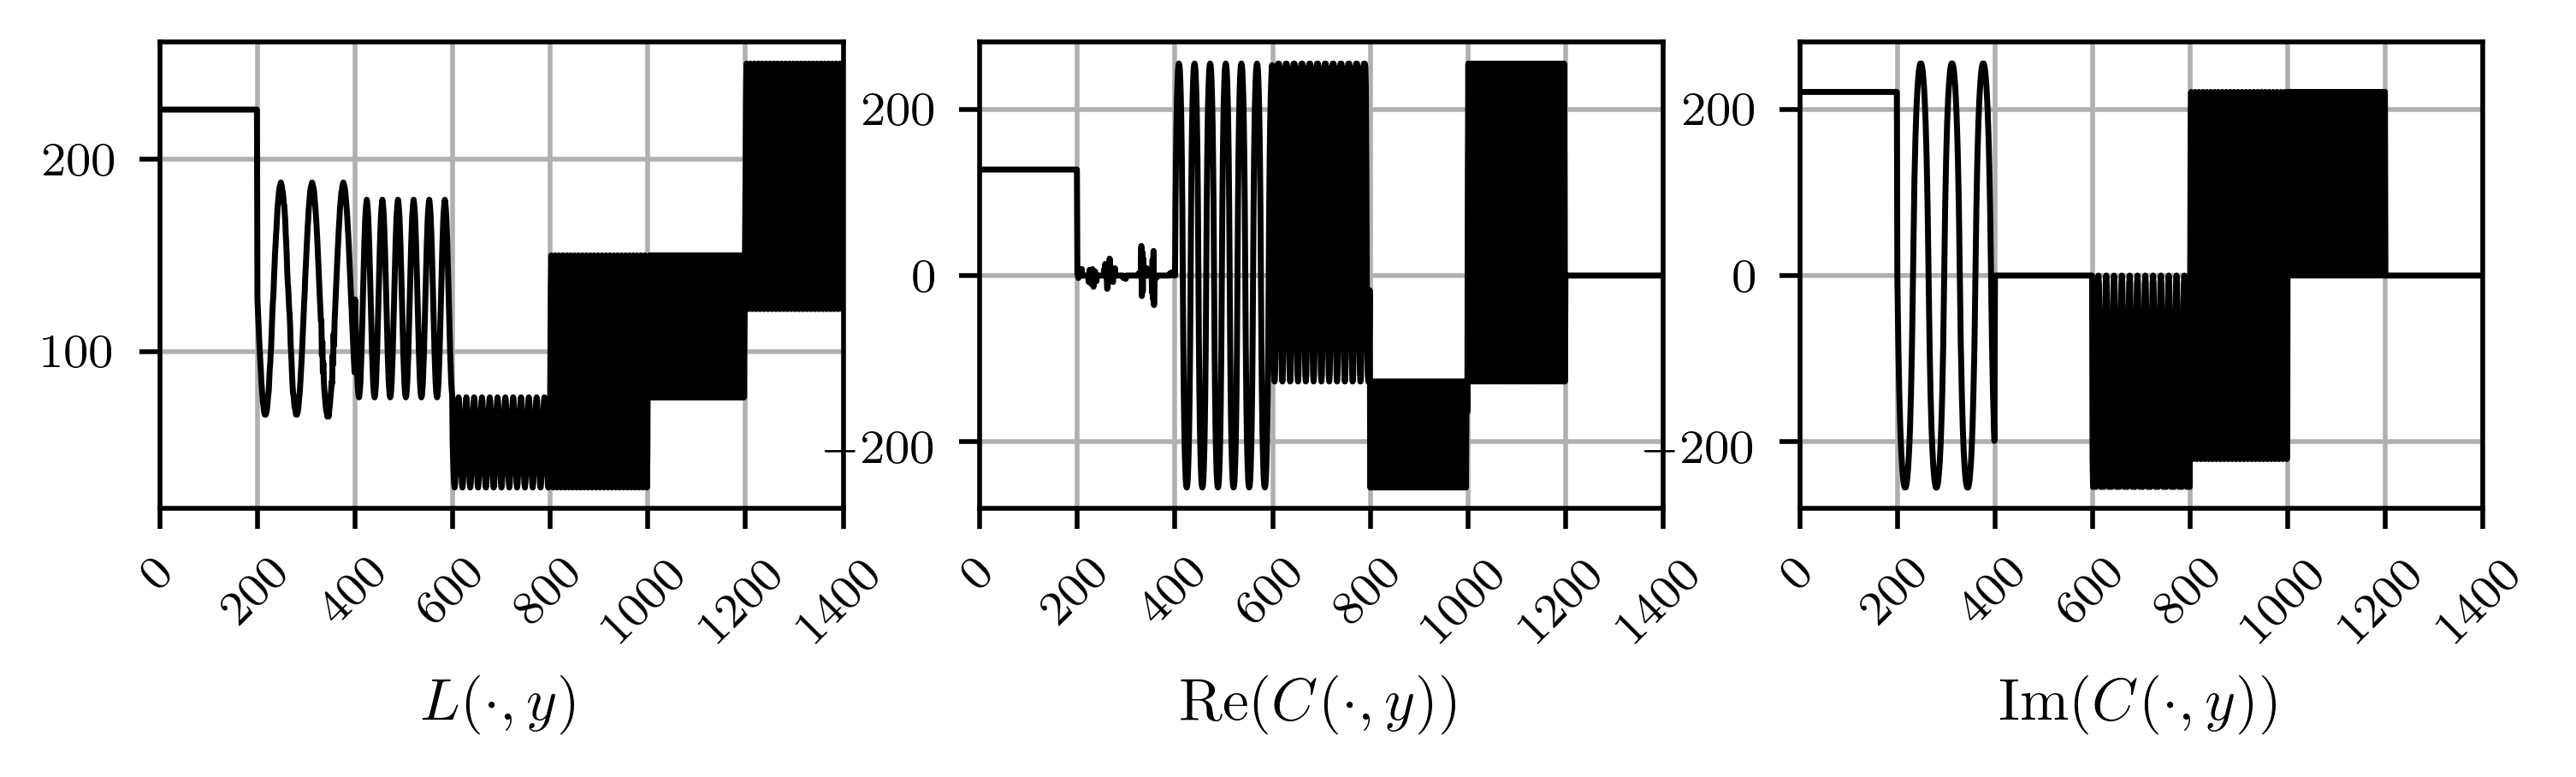
\includegraphics[width=\textwidth]{horizontal_line_three_channel_decomposition}}    
\caption{Illustration of the proposed synthetic image: \captext{(a)} Luminance and chrominance decomposition; \captext{(b)} Numerical values on a horizontal line cut through the three channels.}\label{fig:three_channel_decomposition}
\end{figure}


\subsection{Spectral Image Decomposition}
The first stage of our methodology for color-textured images' characterization consists of representing the input image in a two-channel luminance and chrominance space. Once we represent the image in this space, we obtain the spectral decomposition of each image dimension using a family of optimized Gabor filters (shown in figure \ref{fig:gabrfilter_5f_4a}). Following this strategy, we measure the spatial variations generated by luminance and chrominance individually. 

\begin{figure}[!ht]
    \centering
    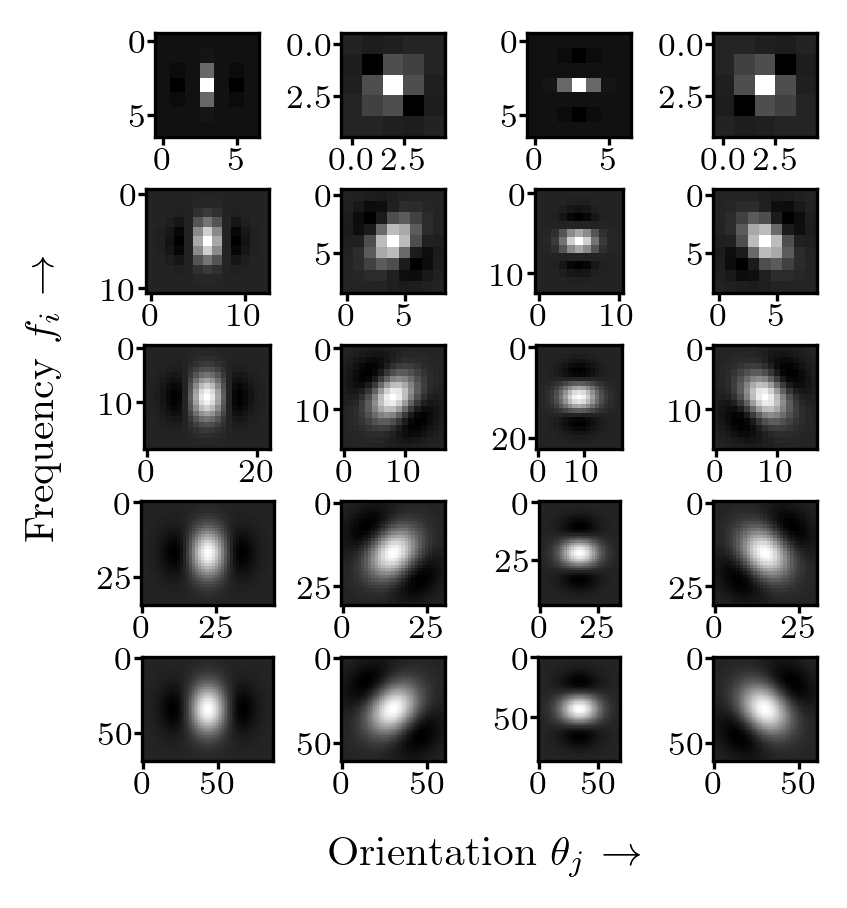
\includegraphics[width=0.6\textwidth]{GaborFilterbank_5f_4a}
    \caption{Gabor filter bank with filters at five frequencies $f$ and four orientations $\theta$ used to model the synthetic image textures.}\label{fig:gabrfilter_5f_4a}    
\end{figure}

Among the different strategies to model the texture information with the Gabor filters listed above, we used the amplitude filter response Eq. \eqref{eq:gabor_magnitude} such that
\begin{equation}\label{eq:gabor_energy}
	e_{c, f, \theta}(x,y) = |r_{c, f, \theta}(x,y)|
\end{equation}
represents the Gabor energy captured by a Gabor filter set at frequency $f$ and orientation $\theta$ for every color channel  $c=\{L, \RE(C), \IM(C)\}$. 

The responses generated by Eq. \eqref{eq:gabor_energy} represent the raw Gabor responses, that is, without any post-processing. Although the Gabor filters we use are optimized (see chapter \ref{ch:spectral_image_decomposition} for more details on filter optimization) to capture the most information by reducing the trade-off between the spatial-frequency domains, the raw responses lack homogeneity, especially at low frequencies, where the filter support is longer. Figure \ref{fig:synthetic_img_gresponses} shows the raw Gabor responses at different frequencies and orientations of the channels of the luminance-chrominance space. 

\begin{figure}[!ht]
    \centering
    \begin{subfigure}[b]{\textwidth}   
        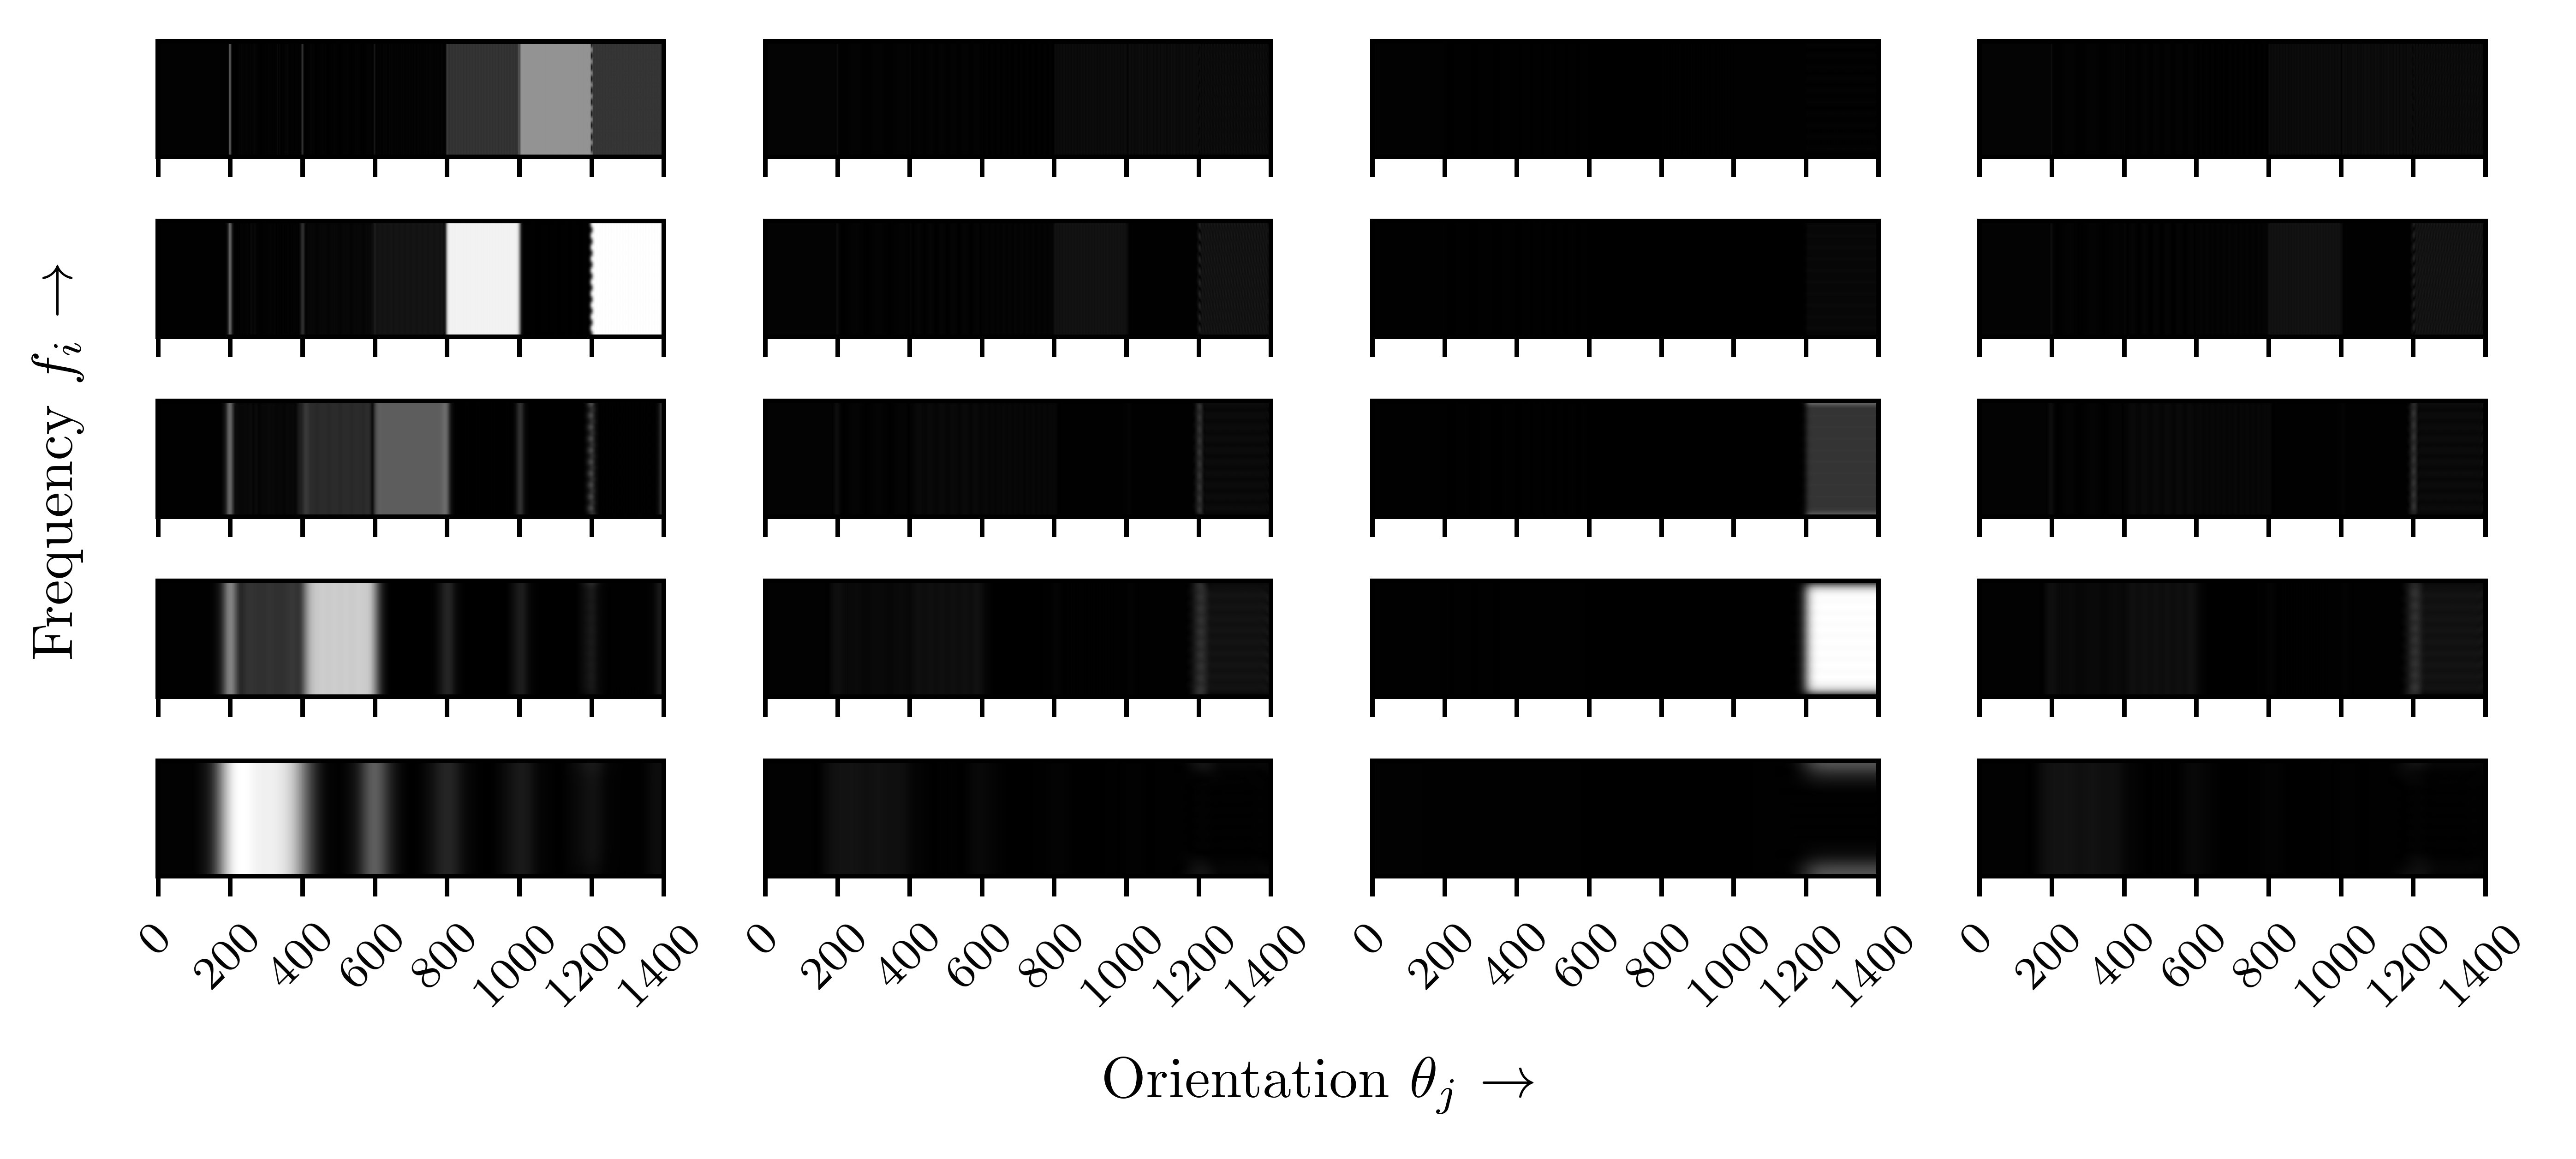
\includegraphics[width=\textwidth]{gabor_resp_lum_synthetic}
        \caption{$e_{L, f, \theta}(x,y)$} 
        \label{fig:lum_raw_gabor_energies}
    \end{subfigure} \\ [2ex]   
    \begin{subfigure}[b]{\textwidth}   
    	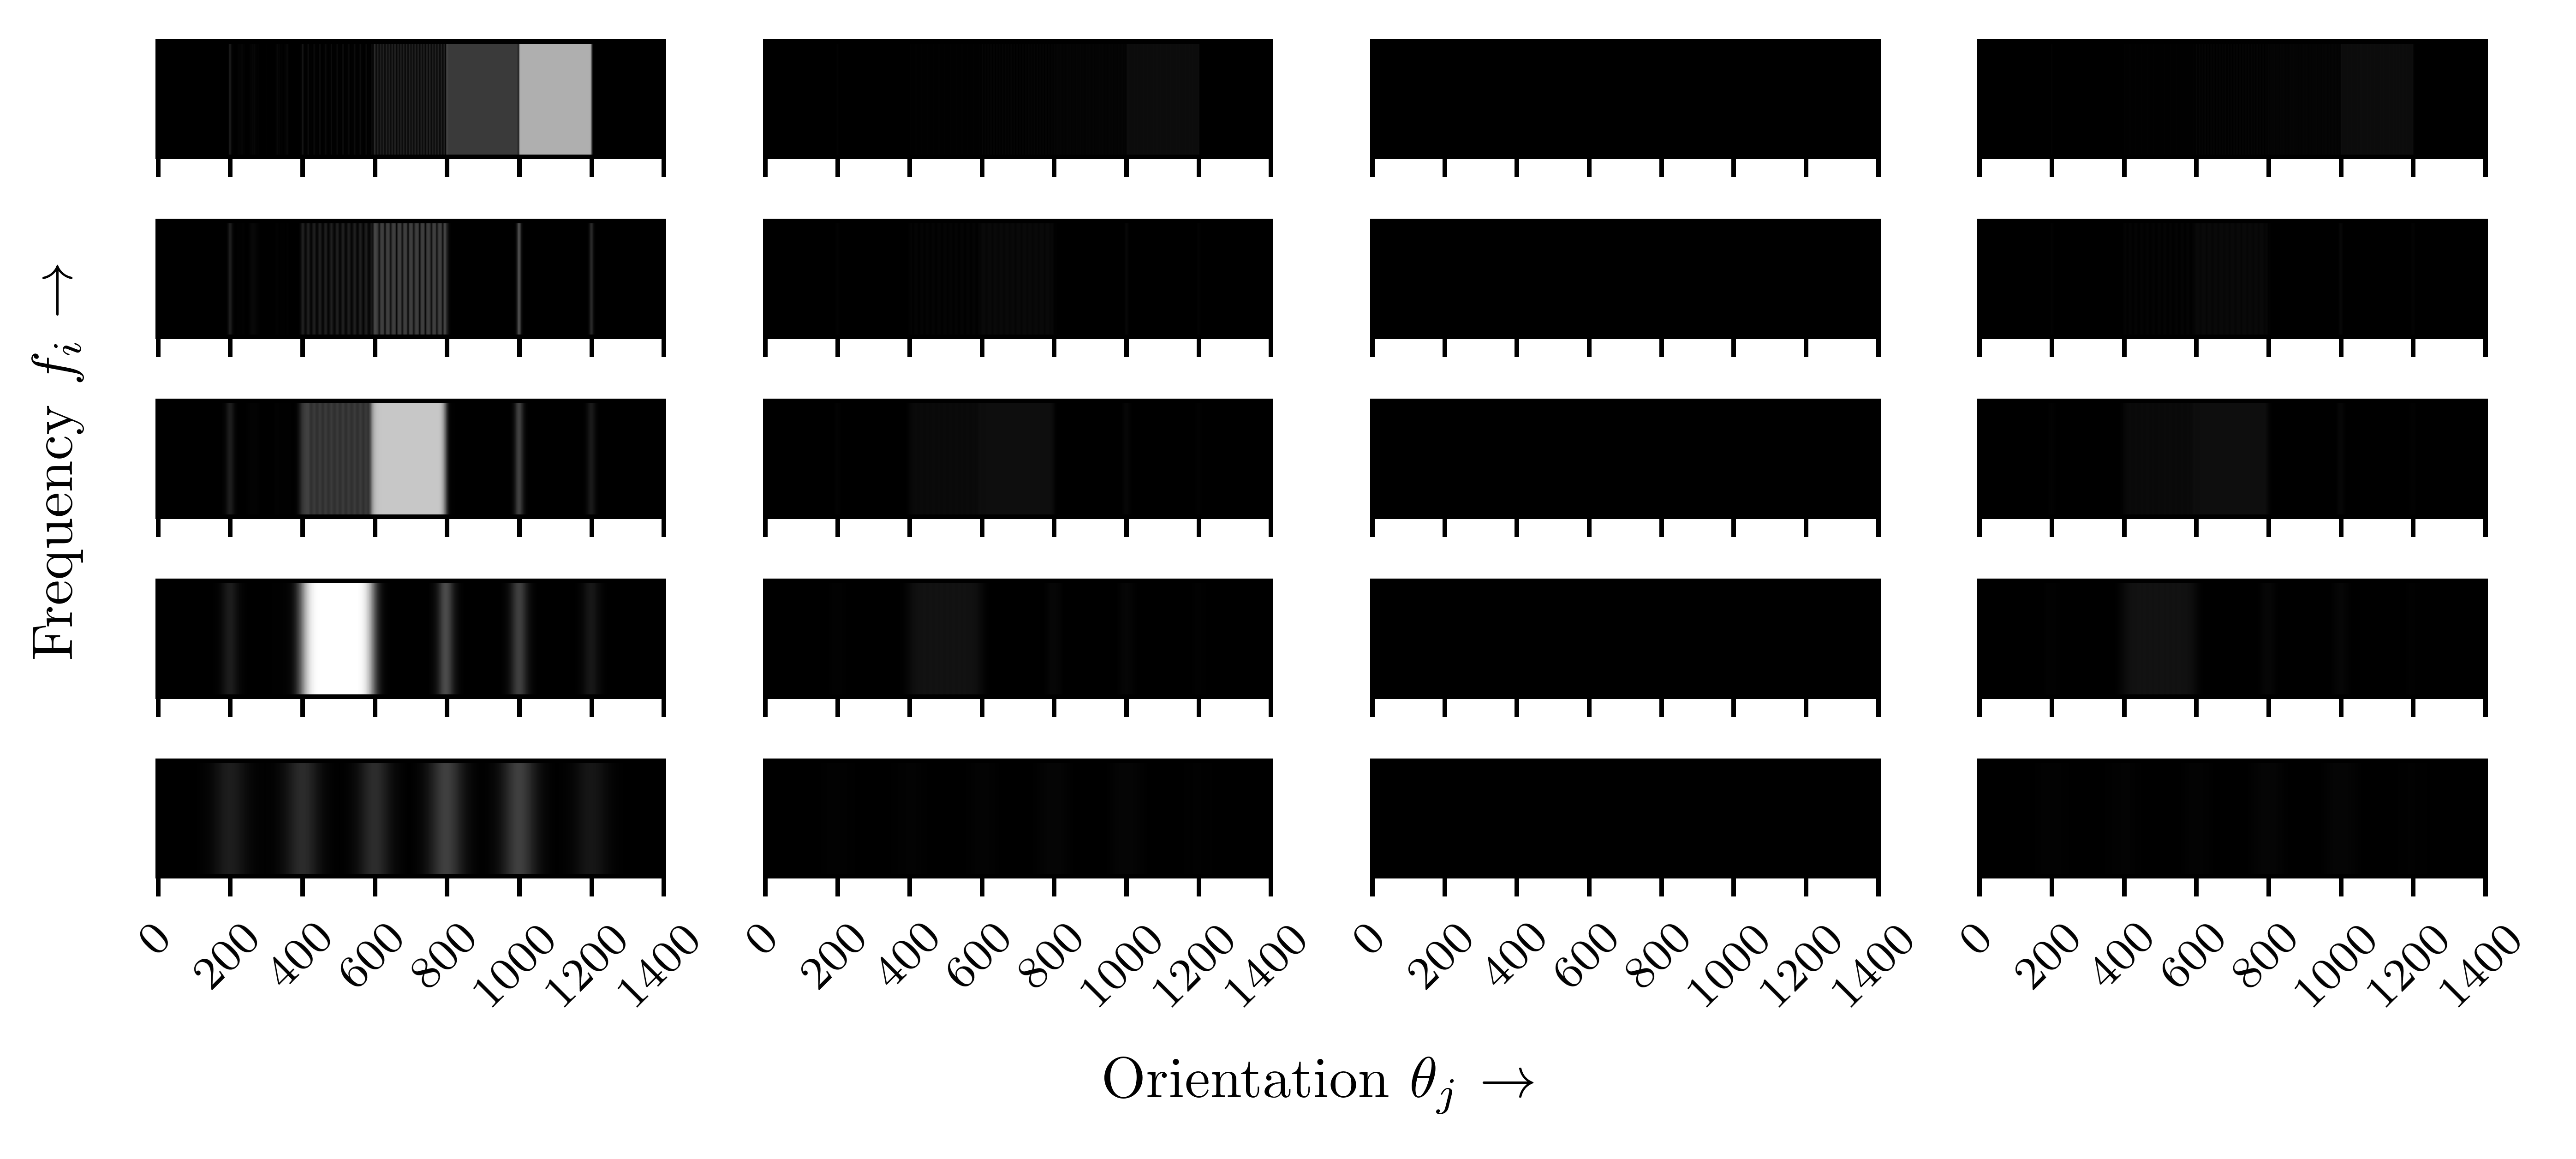
\includegraphics[width=\textwidth]{gabor_resp_cr_synthetic}
    	\caption{$e_{\RE(C), f, \theta}(x,y)$}
        \label{fig:cr_raw_gabor_energies}
    \end{subfigure} \\ [2ex]    	
    \begin{subfigure}[b]{\textwidth}  
        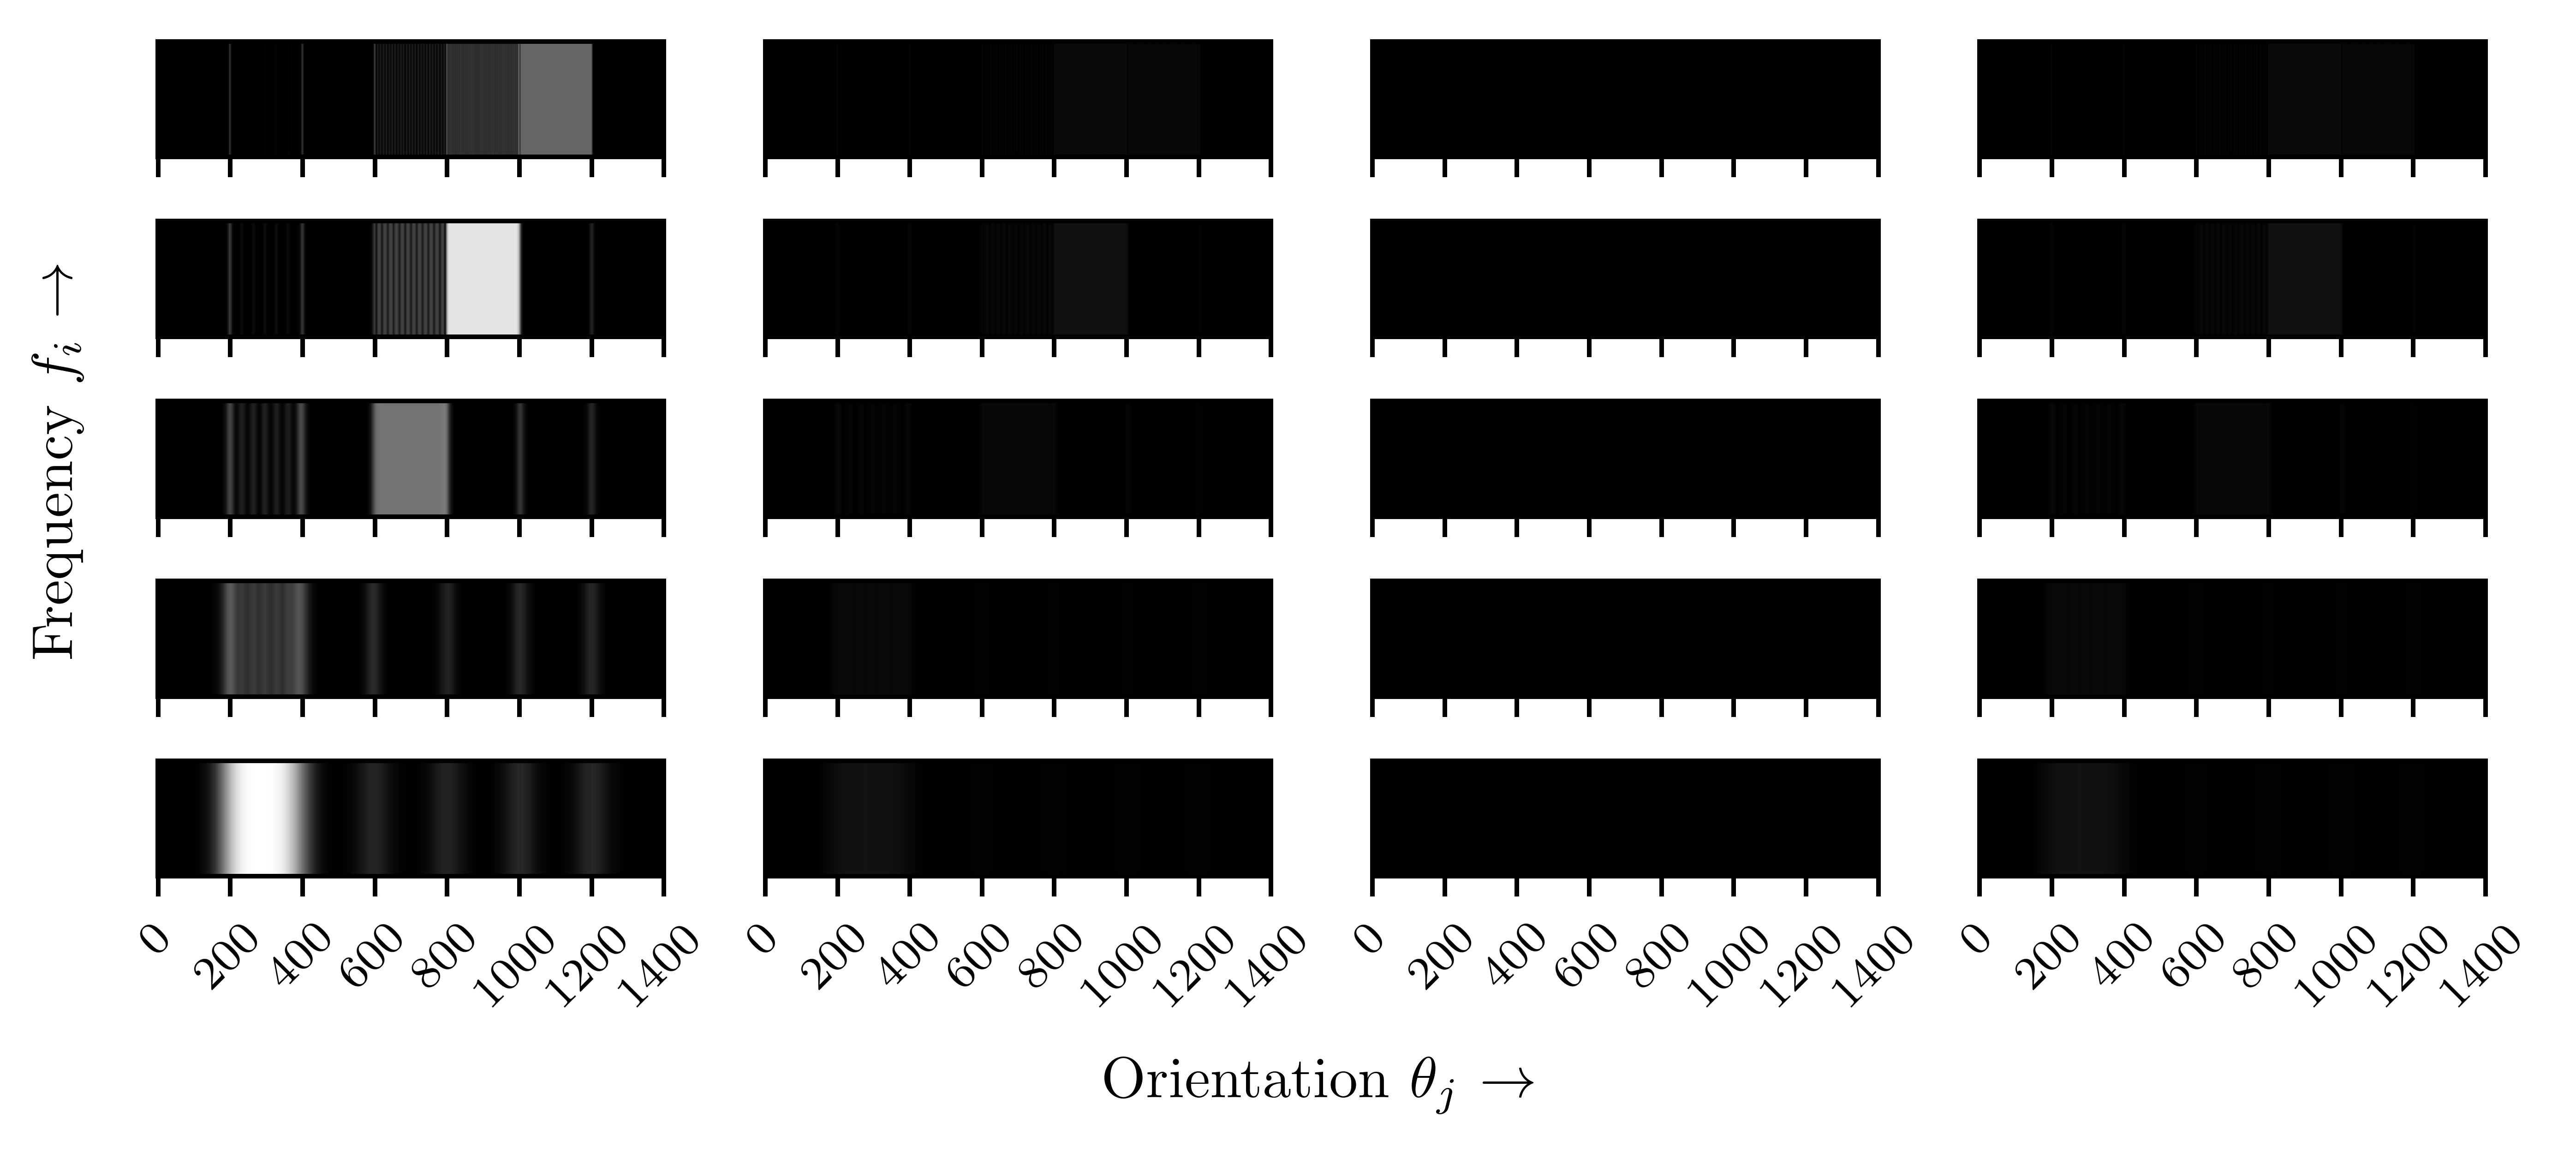
\includegraphics[width=\textwidth]{gabor_resp_ci_synthetic}
        \caption{$e_{\IM(C), f, \theta}(x,y)$}
        \label{fig:ci_raw_gabor_energies} 
    \end{subfigure} 
    	    
    \caption{Gabor responses of the synthetic image obtained with a filter bank of 5 frequencies and 4 orientations. \captext{(a)} Luminance channel responses, \captext{(b)} Real part of chrominance channel responses, \captext{(c)} Imaginary part of chrominance channel responses.}\label{fig:synthetic_img_gresponses}    
\end{figure}

The raw response images are organized as a matrix arrangement that follows the same structure as the Gabor family of filters. The rows in the array represent the responses to the bank's different frequencies (the frequency increases from bottom to top). The array columns represent the responses to the bank's different orientations; from left to right, $\theta$ varies between $ 0^\circ $ $180\circ$ at equidistant intervals. 

In the images of the raw Gabor response array, the zones are brightened more or less depending on the information of the regions. A high level of brightness indicates more energy recovered by the Gabor filter at that frequency and orientation. For example, analyzing the responses of the first column of the luminance channel arrangement shows how the areas light up as the filter frequency changes. The textures' frequency in the synthetic image increases from left to right, while the filter bank's frequency increases from the bottom up, which generates this staircase effect of illuminated areas in the first column of images in subfigure \ref{fig:lum_raw_gabor_energies}.

This same effect is seen when analyzing region 7 of the synthetic image (region with mixed textures at different frequencies and orientations between column pixels 1200 and 1400). The textures of such a region are formed by the alternation of black and white pixels, so all their information is in the luminance channel $L(x, y)$. The vertical texture of the region has frequency $f = 1/8$ and orientation $\theta = 0^\circ$ while the horizontal texture has frequency $f = 1/32$ and orientation $\theta = 90^\circ$. Under this configuration, the response images that reflect the texture information are the image in row 1, column 3  (from bottom to top and left to right) for the horizontal texture and; the response image in row 4, column 1 for the vertical texture. Note that in row 4 of the responses array (corresponding to the frequency $f = 1/8$), we see that region 5 is illuminated with the same intensity as region 7, which indicates that both zones contain textures at that frequency. This information is consistent with the description of the regions of our synthetic image.

Another interesting thing visible in the Gabor responses is that region 1 of the synthetic image (region without texture between pixels 0 and 200) does not illuminate any channel or any frequency or orientation of the filters. This effect occurs because Gabor filters only retrieve the texture information of the image. Color information is implicit in the chrominance channel. We see this reflected in the responses of the real and imaginary channels of the chrominance subfigures \ref{fig:cr_raw_gabor_energies}, \ref{fig:ci_raw_gabor_energies}. 


\subsubsection{Refinement of Gabor responses}

Although the raw Gabor responses are a good starting point for describing textures, these responses exhibit a lack of spatial homogeneity generated by the trade-off between the spatial-frequency domains of the Gabor filters (see chapter \ref{ch:gabor_filter_description} and appendix \ref{ch:uncertainty_principle} for more details about the uncertainty principle in Gabor filters and the optimization of  Gabor filters proposed in this thesis). Clearly this behavior is more visible at high frequencies, where the support of Gabor filters is smaller. For example in the responses of the imaginary channel of the chrominance corresponding to the frequency $f=1/8$ and orientation $\theta = 0^\circ$ (response image at row 1 column 1 in subfigure \ref{fig:ci_raw_gabor_energies} , we see how the energy found by the filter for the region 4 (between pixels 400 and 600) is not homogeneous, and the lines texture effect keeps appearing.

In the literature there are various strategies to homogenize the filter responses, one of them very recurrent is the application of a non-linear transformation \citep{Jain.Farrokhnia:IJPR:1991}. This nonlinear transformation acts as the bounded sigmoid activation function used in artificial neural networks. The non-linear transformation modulates the sinusoidal signals of the image to square signals, so it behaves like a blob detector. The downside to this approach is that we need to define a empirical parameter that functions as a threshold for the transformation.

We propose to use a morphological opening to achieve homogenization of the Gabor responses. The opening is defined as
\begin{equation}\label{eq:gabor_energy_opn}
	\widehat{e}_{c, f, \theta}(x,y) = \gamma_B(e_{c, f, \theta}(x,y)) 
\end{equation}
where $B$ is the structuring element and $\gamma_B$ is the morphological opening. Our approach's advantage is that the structural element's size is defined individually for each Gabor energy by the central period $ T=1 / f $ of each filter. For example, the radius of a disk-shaped structuring element for the Gabor energies obtained with a filter with a center frequency $ f = 1/8 $ is 8 pixels. Gabor responses after morphological opening appear in the figure \ref{fig:synthetic_img_gresponses_opn}.
%\gamma_B(e_{c, f, \theta}(x,y)) = \delta_B[\varepsilon_B(e_{c, f, \theta}(x,y)] defined as an erosion followed by a dilation using the same structuring element $B$ for both operations.
\begin{figure}[!ht]
    \centering
    \begin{subfigure}[b]{\textwidth}   
        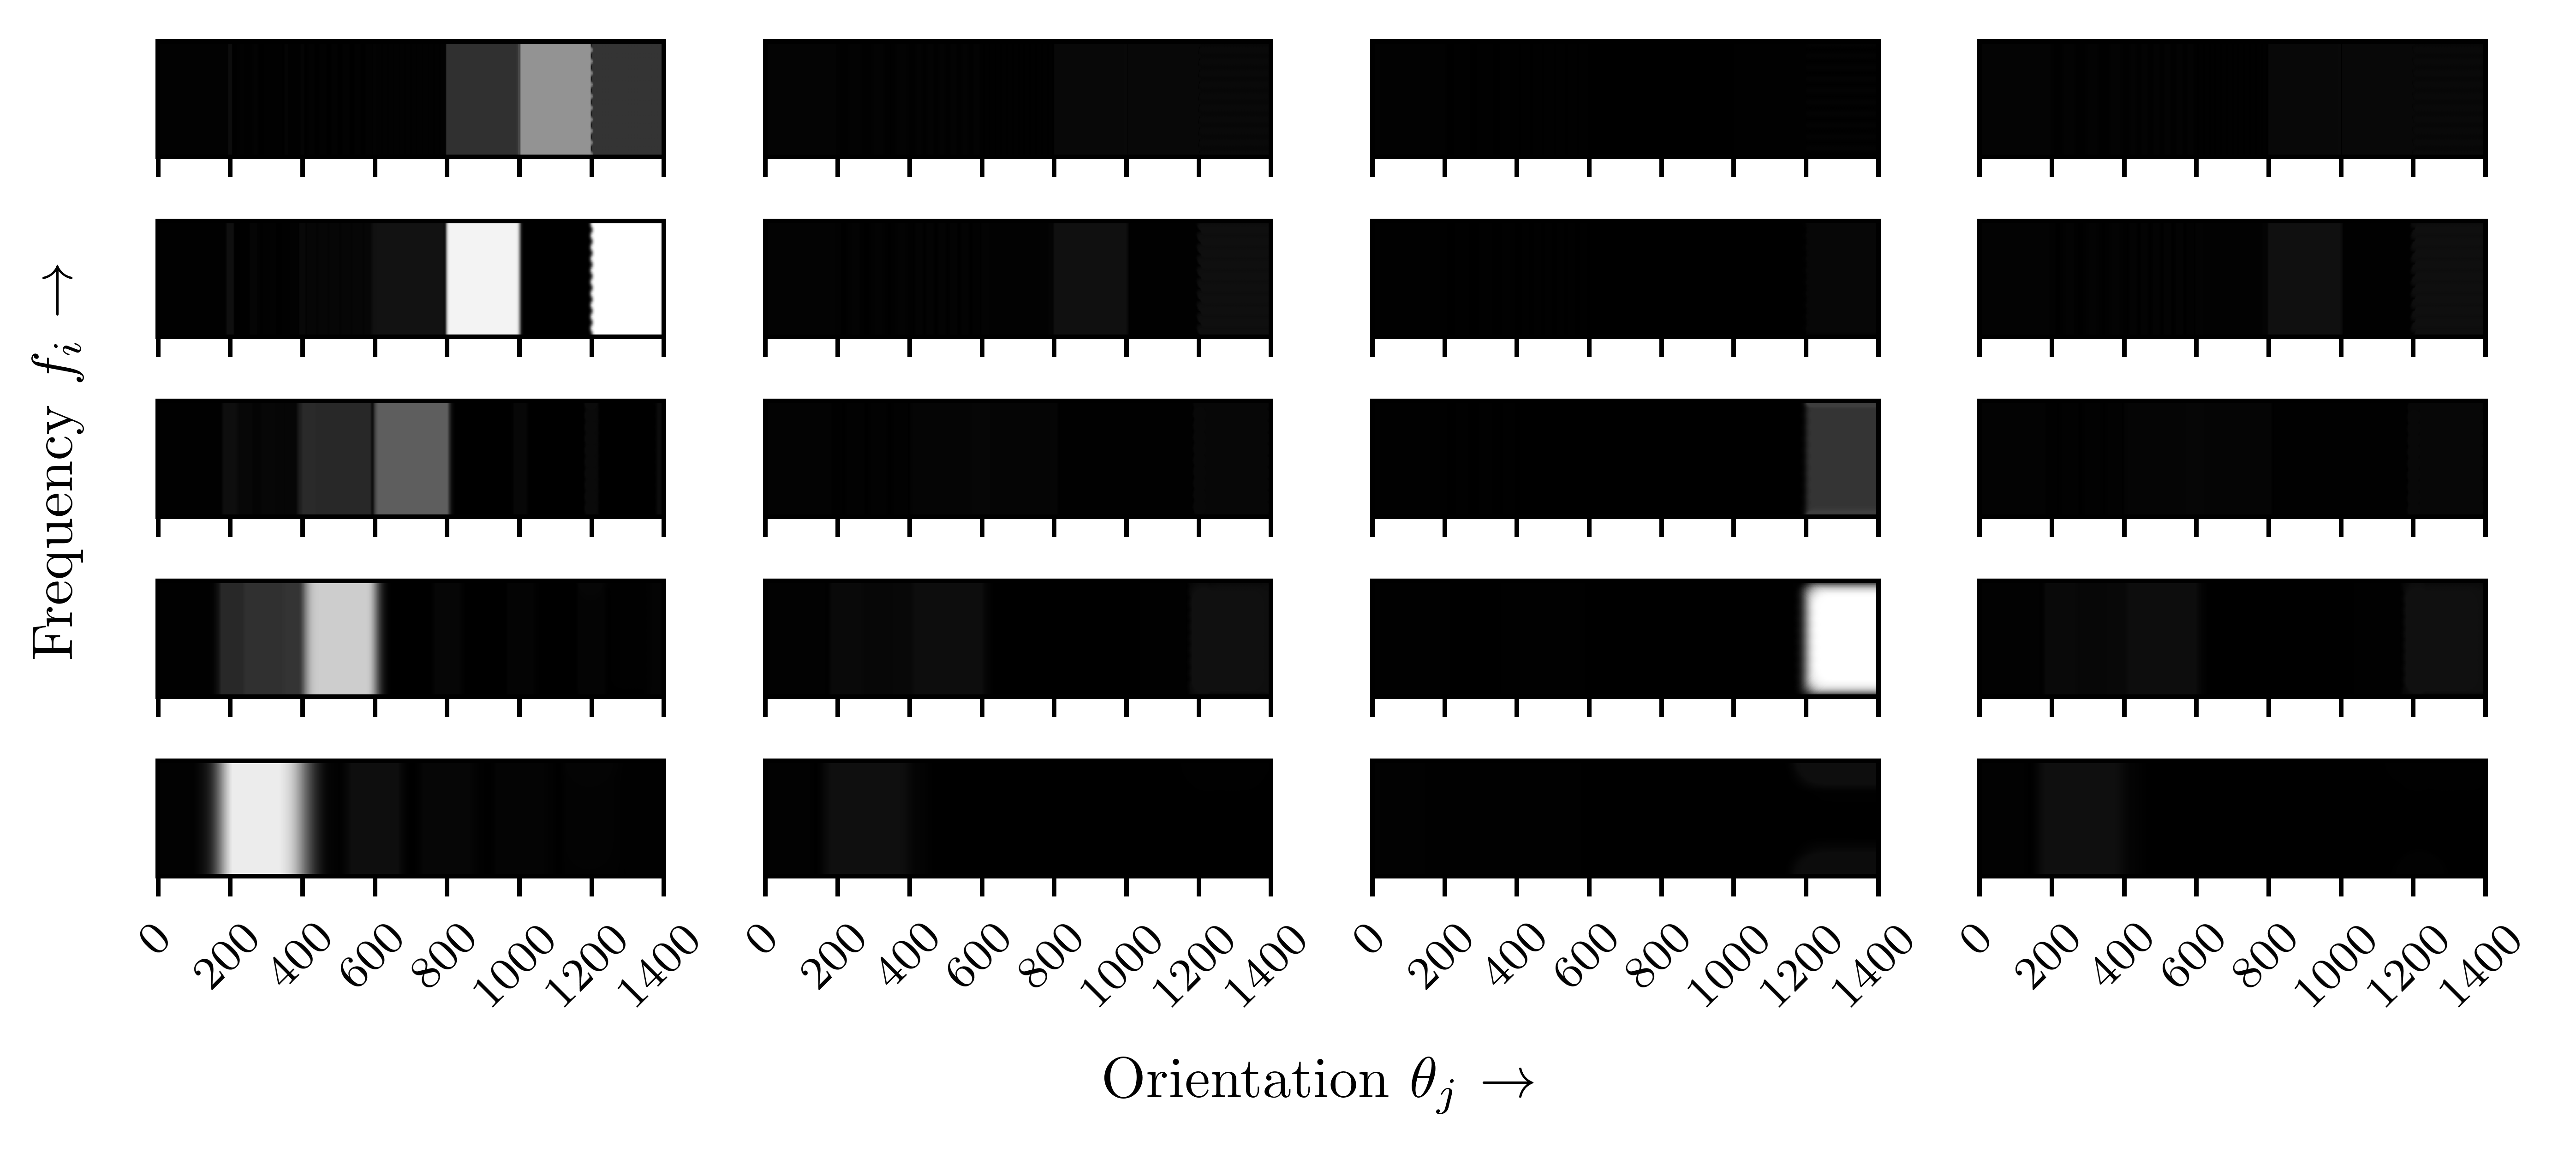
\includegraphics[width=\textwidth]{gabor_resp_lum_synthetic_opn}
        \caption{$\widehat{e}_{L, f, \theta}(x,y)$} 
        \label{fig:lum_gabor_energies_opn}
    \end{subfigure} \\ [2ex]   
    \begin{subfigure}[b]{\textwidth}   
    	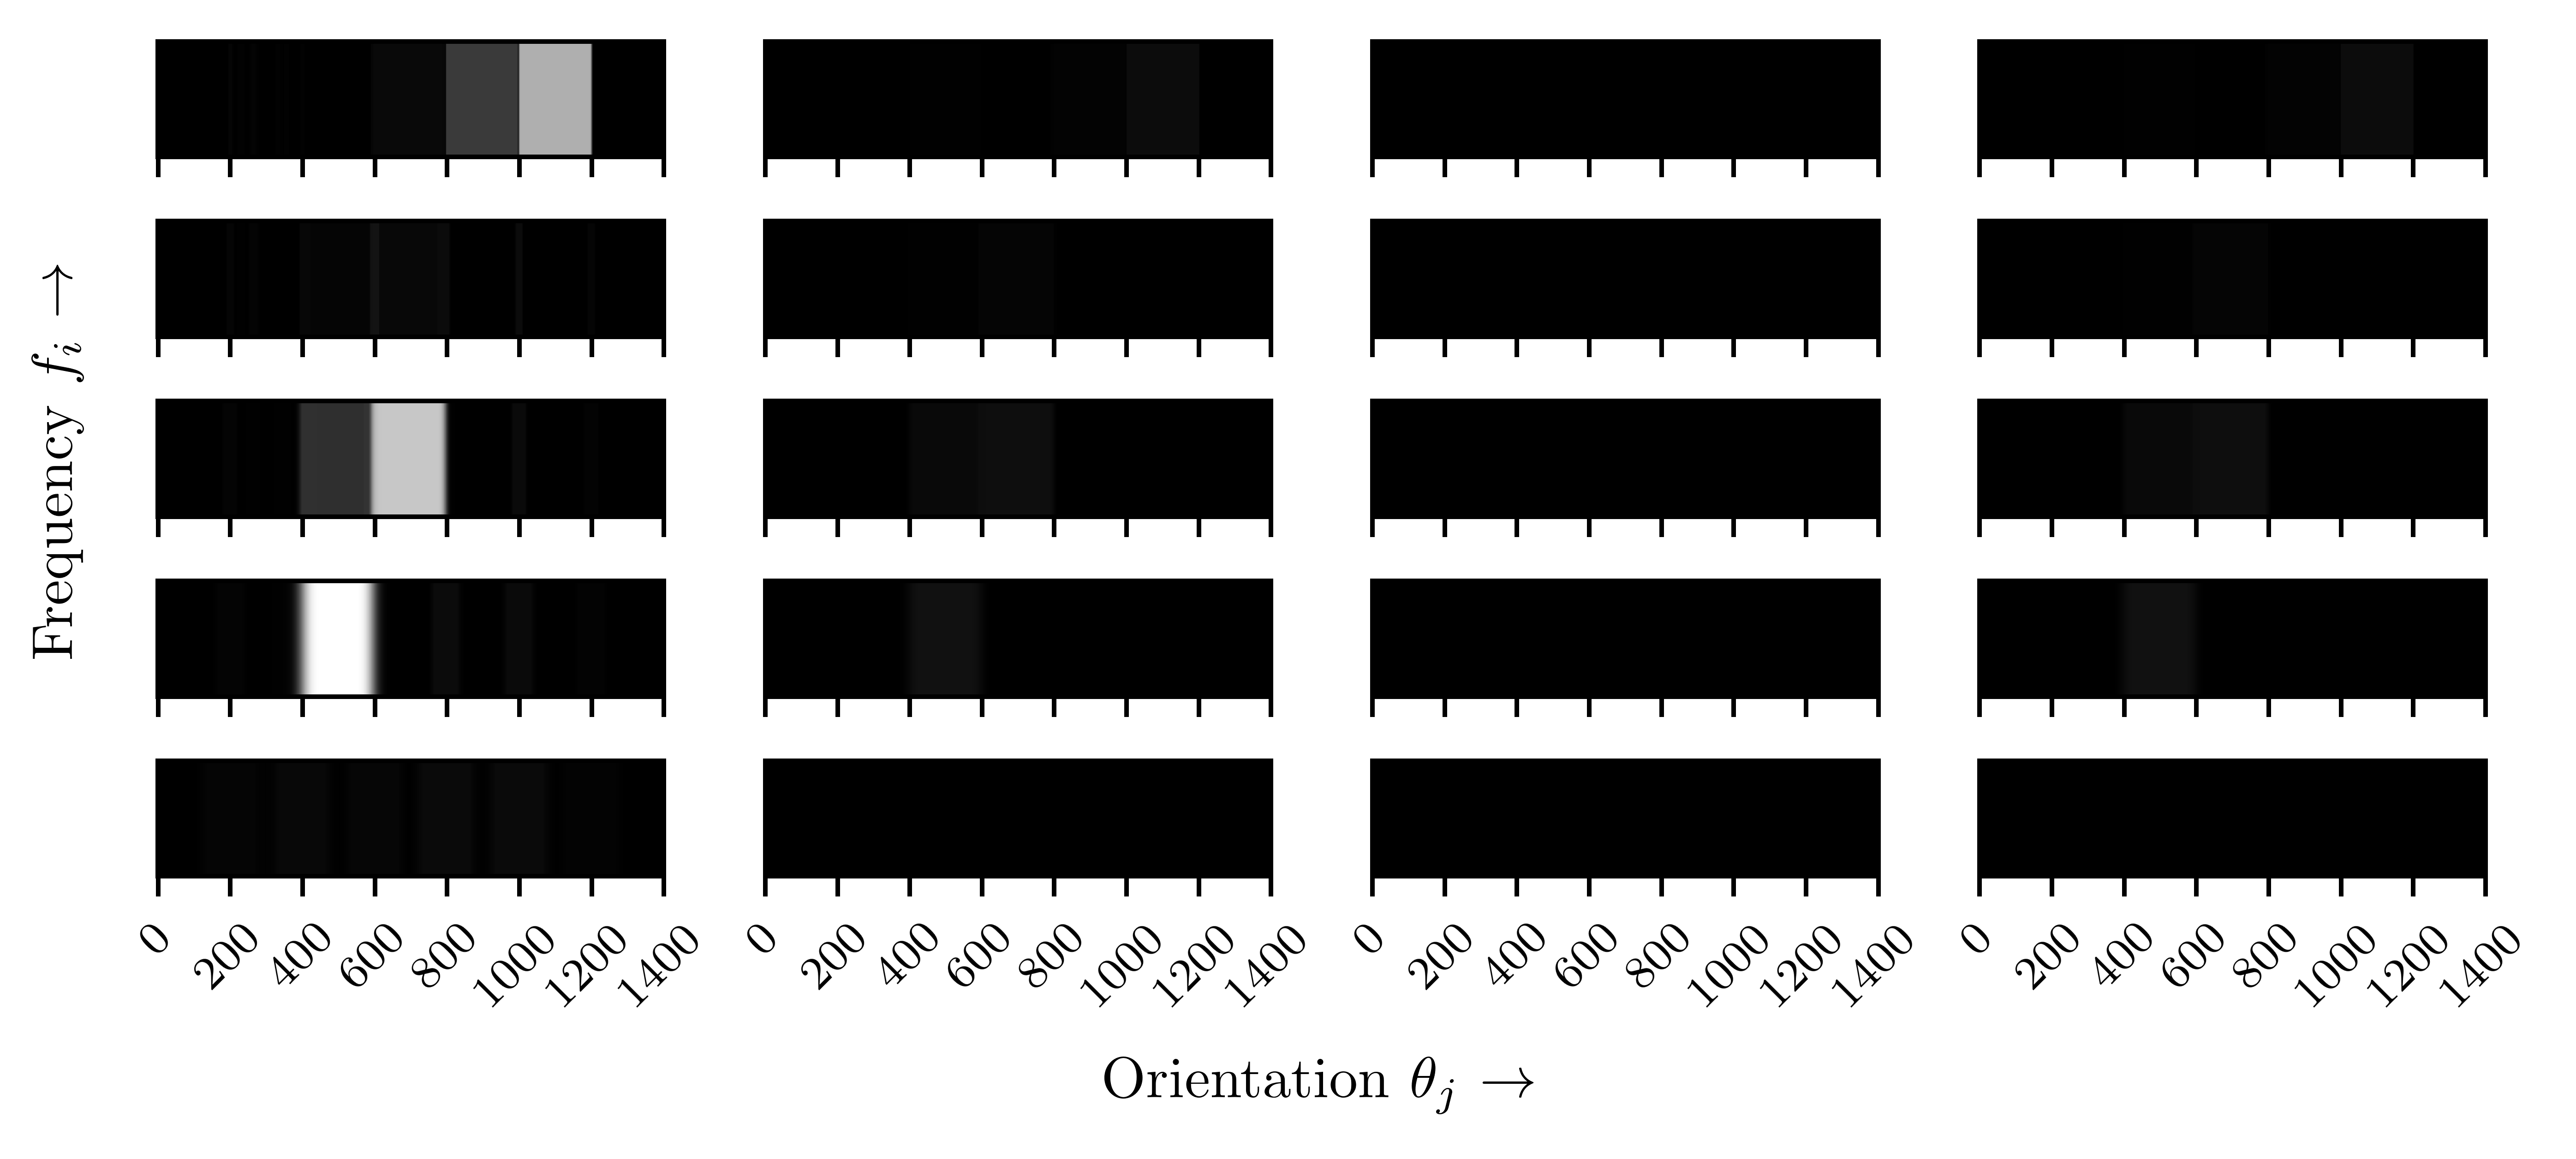
\includegraphics[width=\textwidth]{gabor_resp_cr_synthetic_opn}
    	\caption{$\widehat{e}_{\RE(C), f, \theta}(x,y)$}
        \label{fig:cr_gabor_energies_opn}
    \end{subfigure} \\ [2ex]    	
    \begin{subfigure}[b]{\textwidth}  
        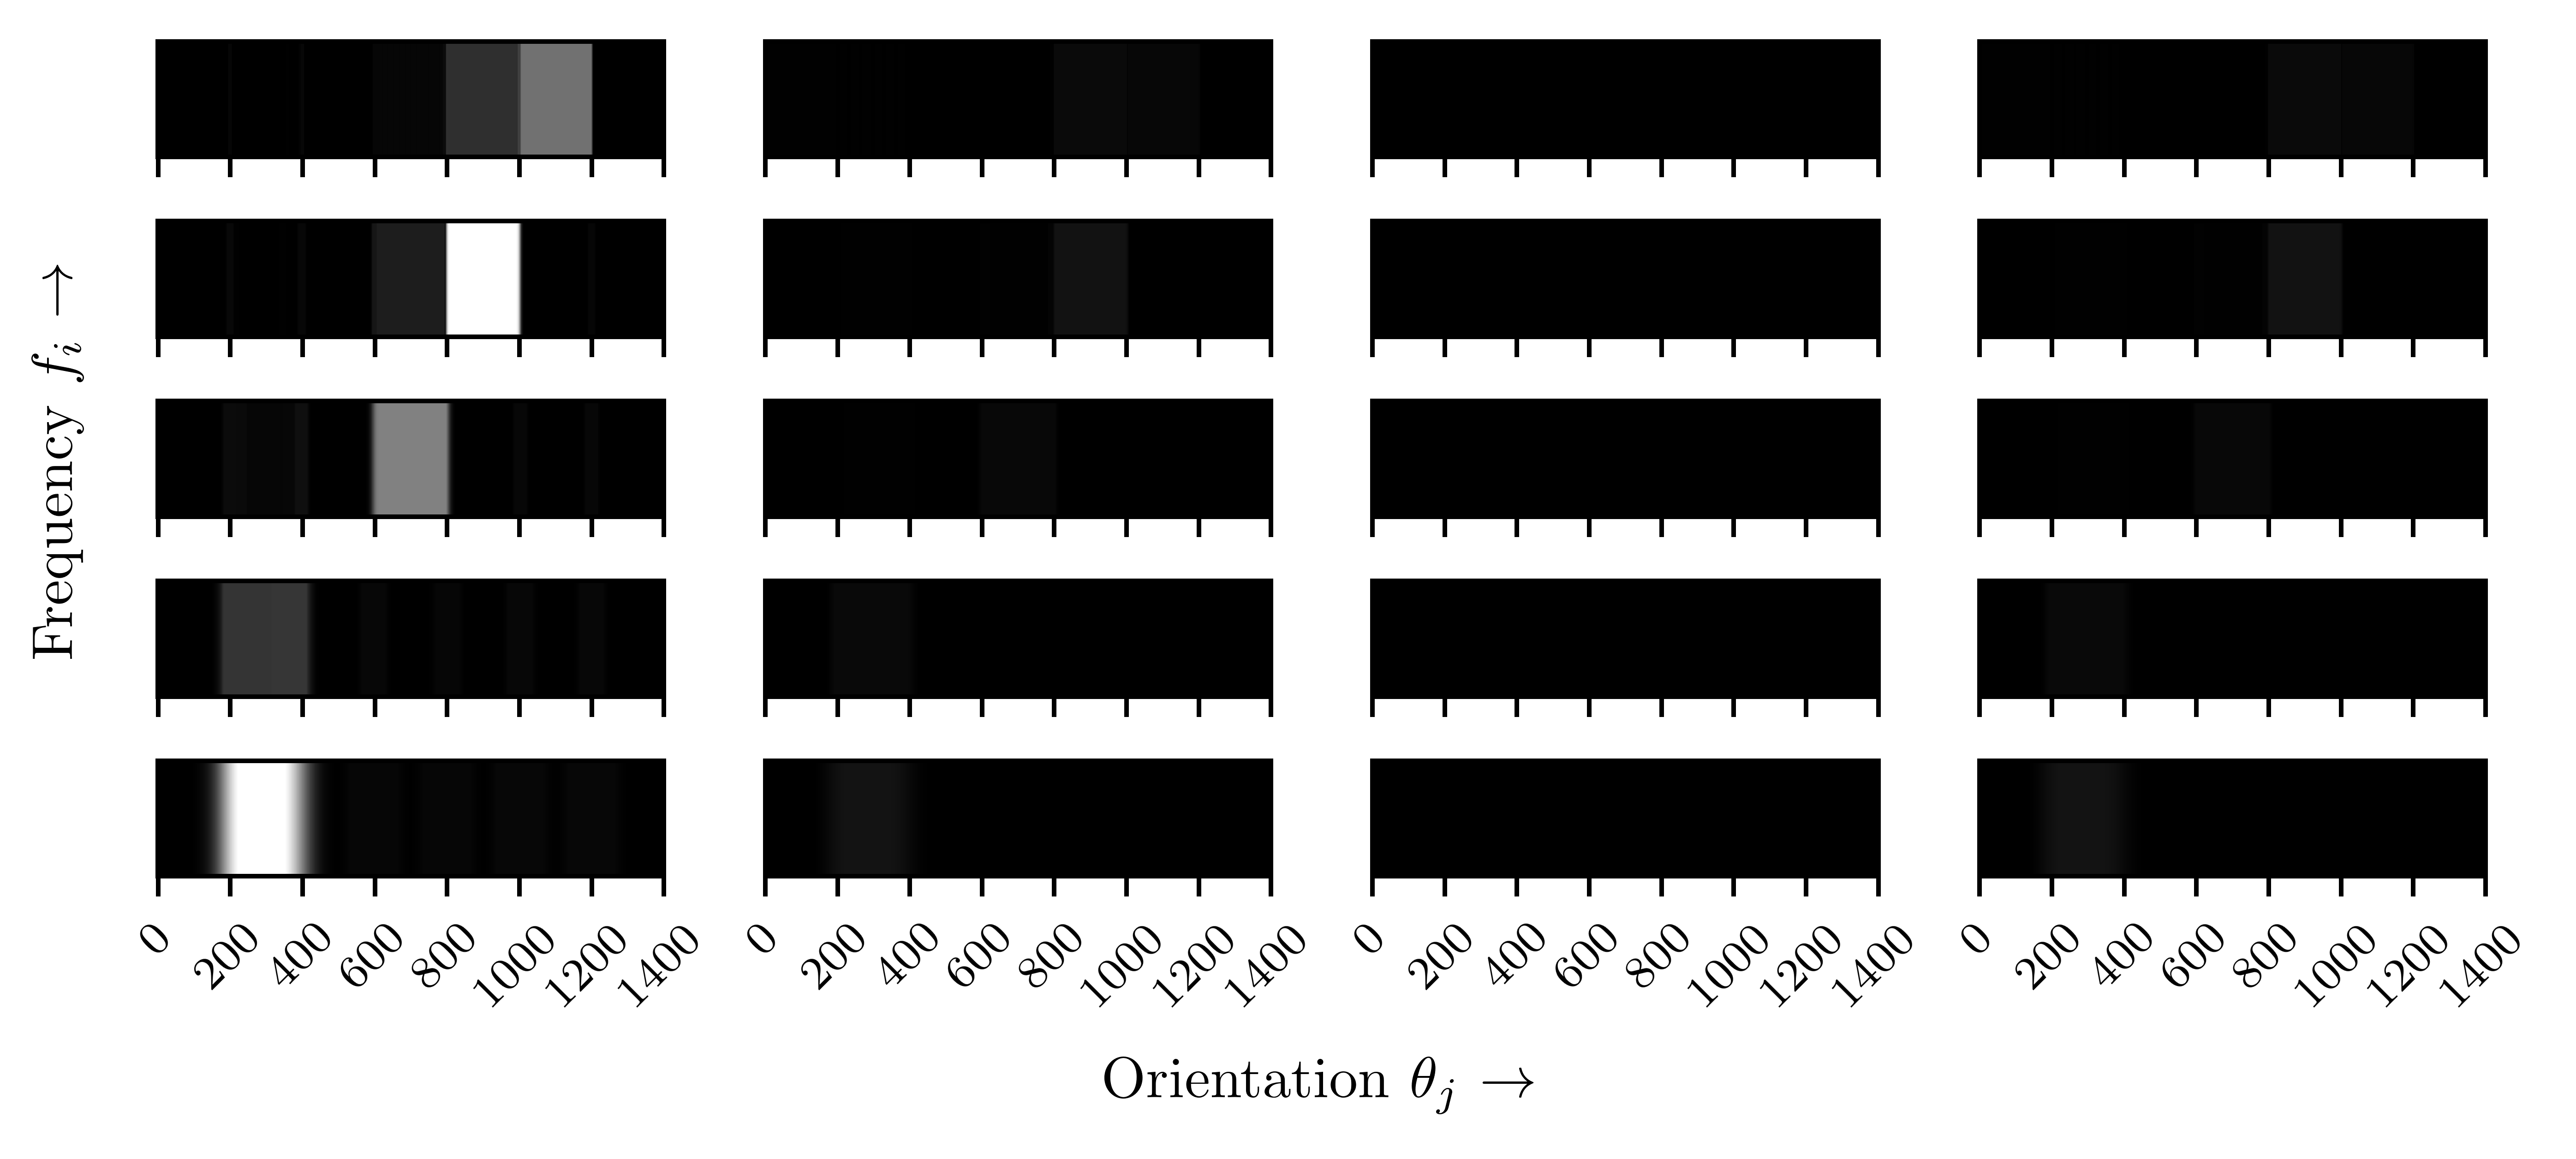
\includegraphics[width=\textwidth]{gabor_resp_ci_synthetic_opn}
        \caption{$\widehat{e}_{\IM(C), f, \theta}(x,y)$}
        \label{fig:ci_gabor_energies_opn} 
    \end{subfigure} 
    	    
    \caption{Gabor responses after the morphological openning of the synthetic image. \captext{(a)} Luminance channel responses, \captext{(b)} Real part of chrominance channel responses, \captext{(c)} Imaginary part of chrominance channel responses.}\label{fig:synthetic_img_gresponses_opn}    
\end{figure}

Finally, after the morphological opening, we apply an adaptive Gaussian smoothing to calculate the Gabor energy locally. This smoothing is defined as 
\begin{equation}\label{eq:gabor_energy_smth}
	\widetilde{e}_{c, f, \theta}(x,y) = w(x, y)_\sigma\ast \widehat{e}_{c, f, \theta}(x,y)
\end{equation}
where the scale parameter $\sigma$ of the Gaussian window $W(x,y)_\sigma$ is the maximum between value between the standard deviations of the Gabor filter support in the $x$ and $y$ axis.
\begin{equation}\label{eq:gauss_sigma_smth}
	\sigma = \mathrm{max}(\sigma_x, \sigma_y)
\end{equation}

From the analysis of Gabor filters presented in chapter \ref{ch:gabor_filter_description}, we know that the standard deviations $\sigma_x, \sigma_y$ (Eq. \eqref{eq:1D_Gaussian_envelope_width}) of a Gabor filter are defined by its center frequency $f$ and the frequency and angular point crossing points (Eqs. \eqref{eq:crossing_point}, \eqref{eq:orientation_interval_crossing_point}) defined at the moment of filter bank design. Figure \ref{fig:synthetic_img_gresponses_opn_smth} shows the Gabor responses after opening and adaptive Gaussian smoothing. 

\begin{figure}[!ht]
    \centering
    \begin{subfigure}[b]{\textwidth}   
        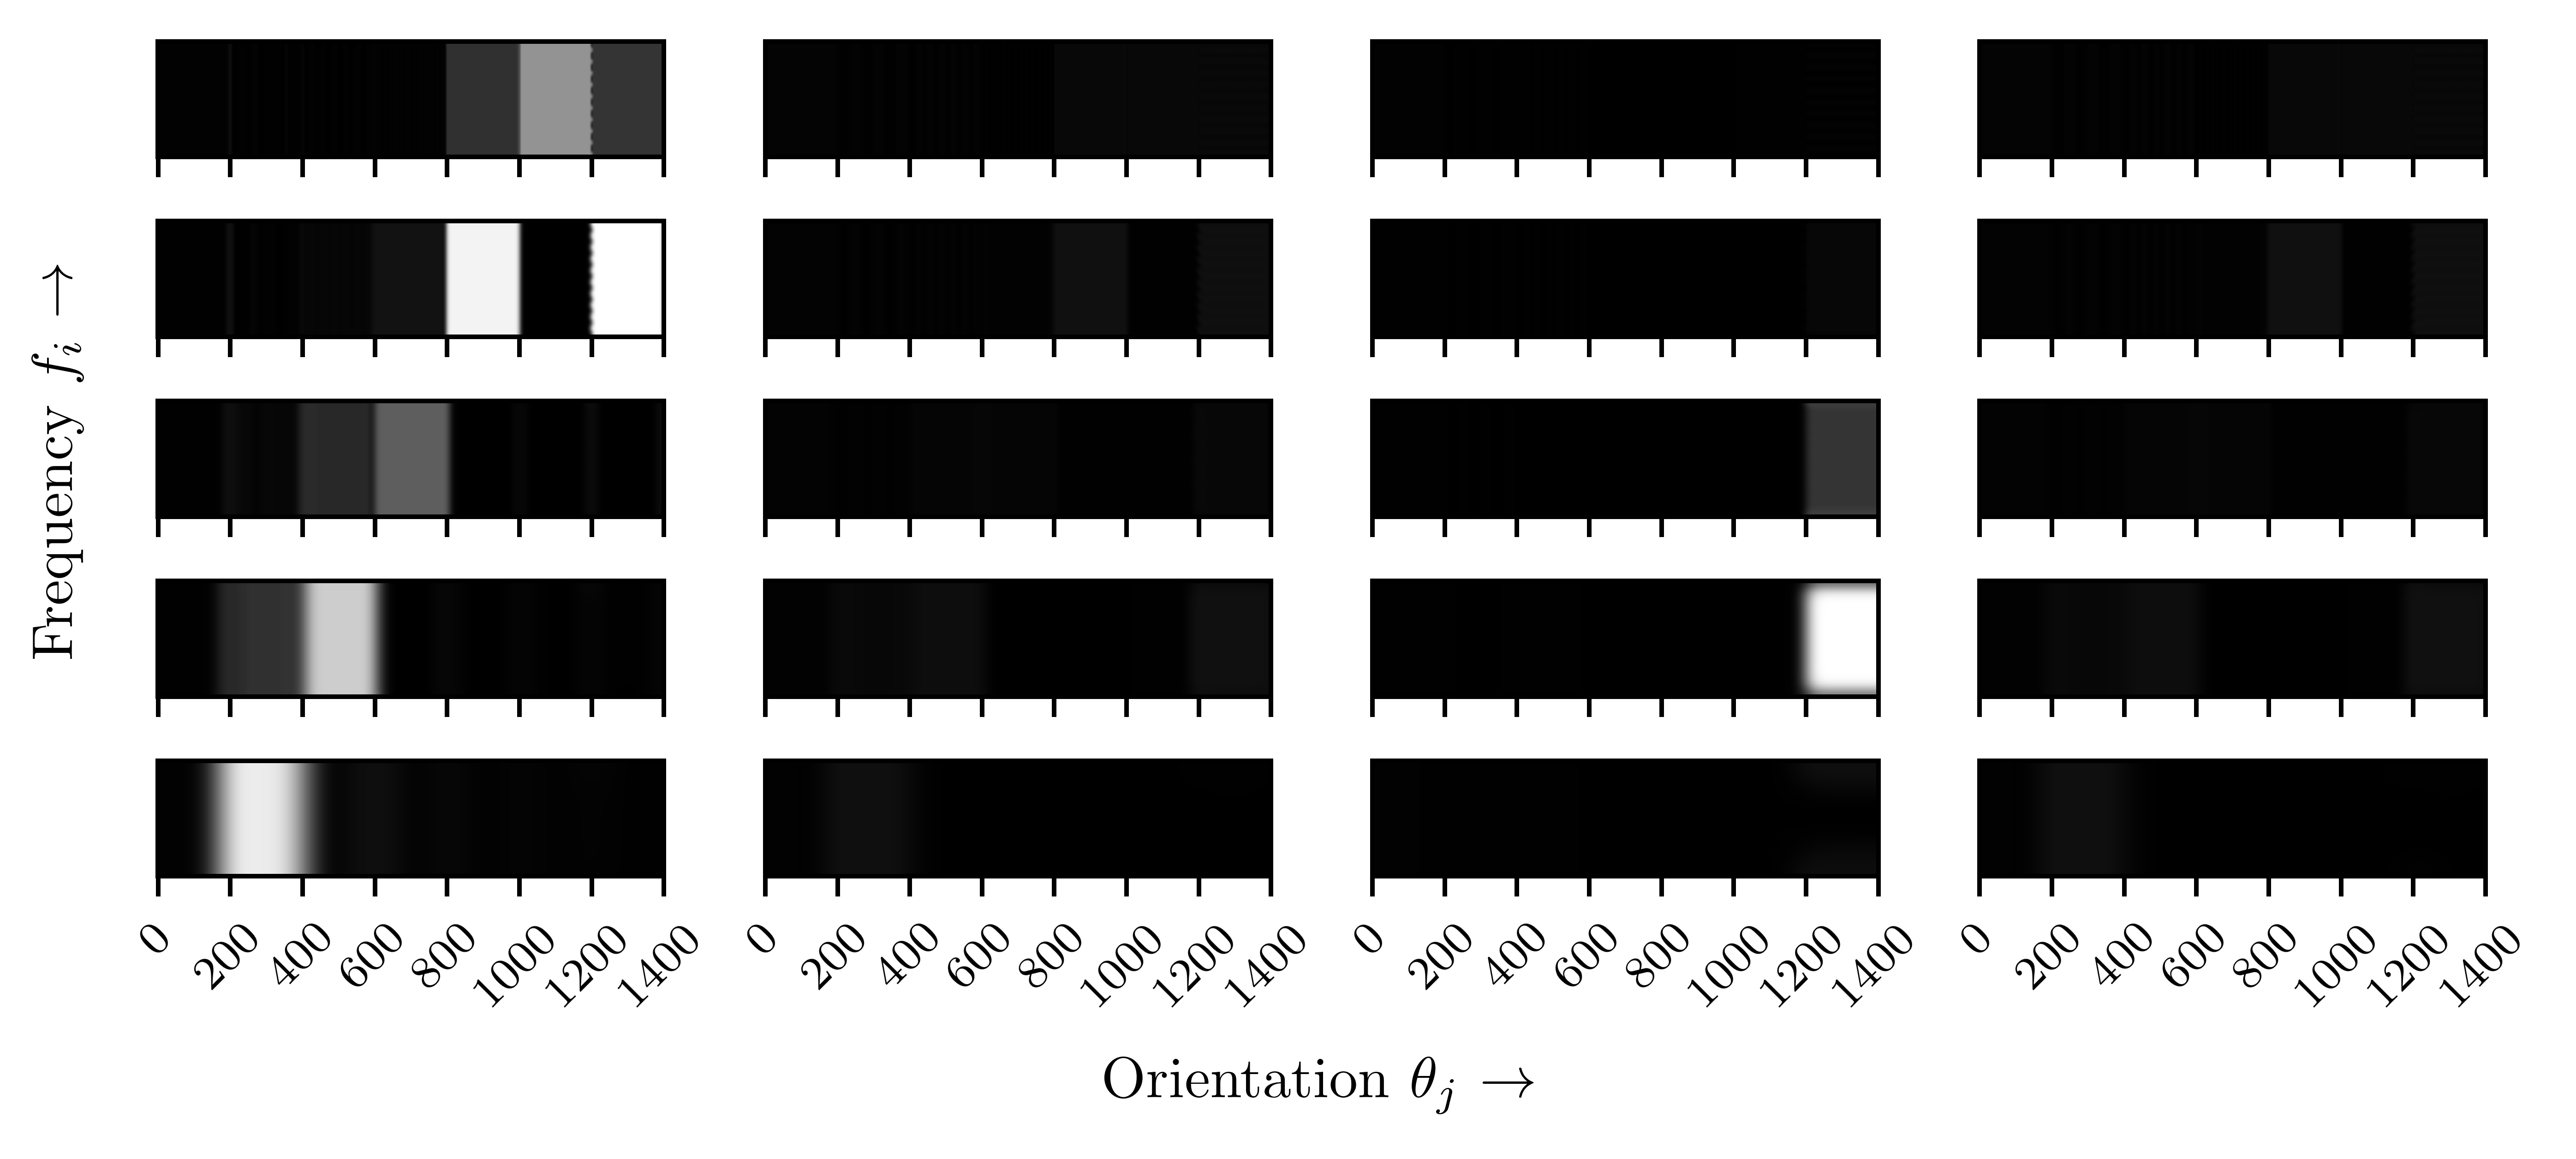
\includegraphics[width=\textwidth]{gabor_resp_lum_synthetic_opn_smth}
        \caption{$\widetilde{e}_{L, f, \theta}(x,y)$} 
        \label{fig:lum_gabor_energies_opn_smth}
    \end{subfigure} \\ [2ex]   
    \begin{subfigure}[b]{\textwidth}   
    	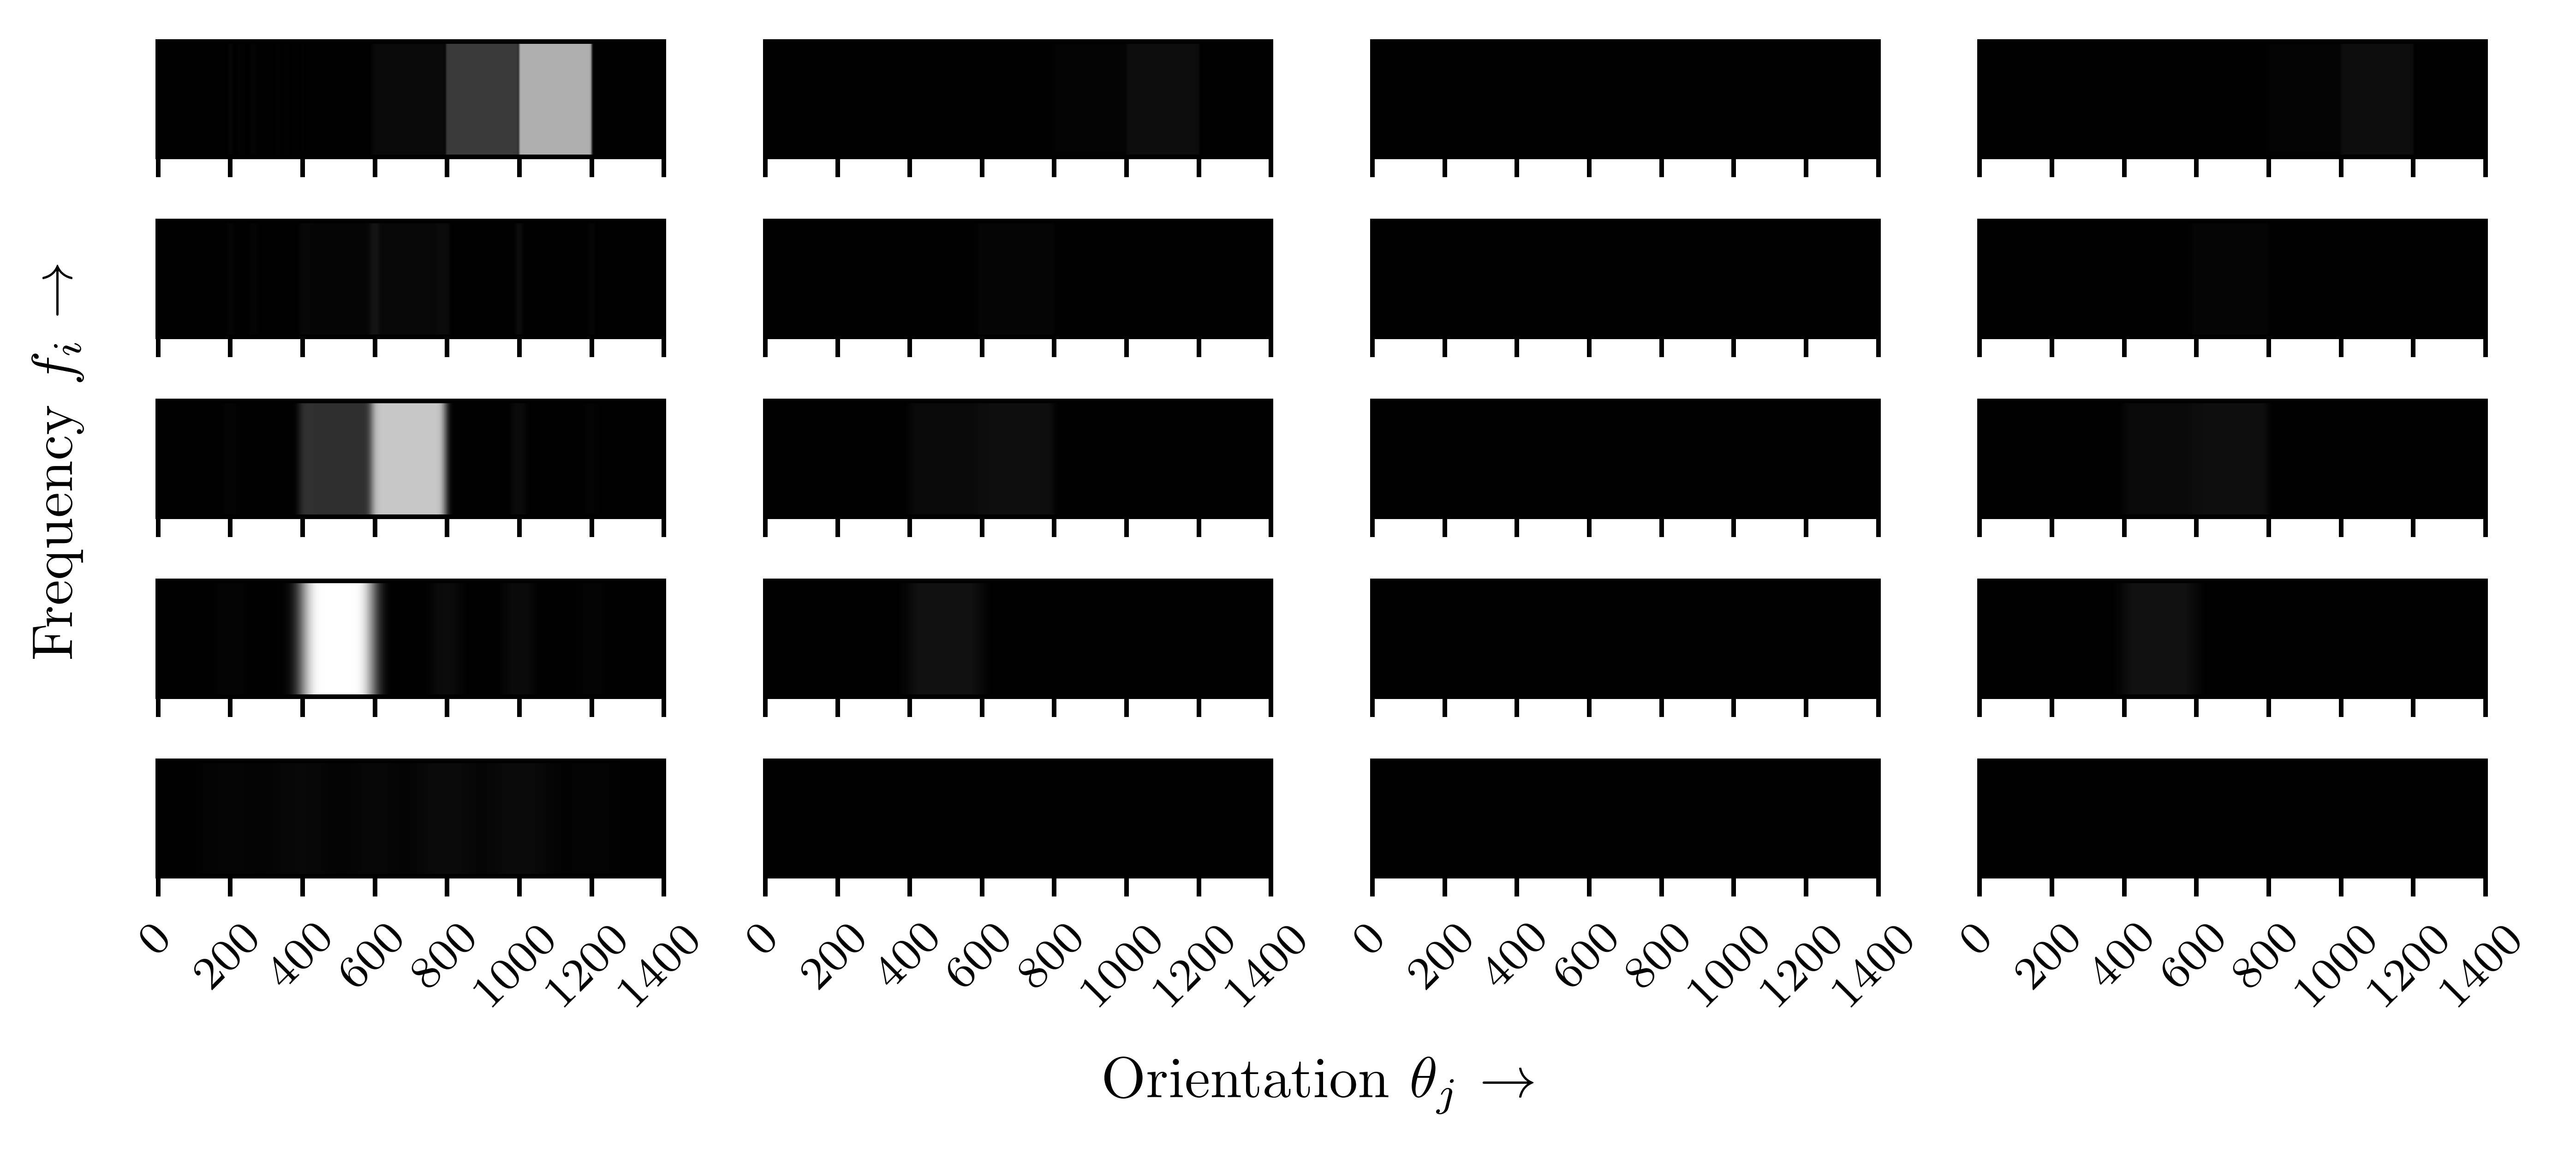
\includegraphics[width=\textwidth]{gabor_resp_cr_synthetic_opn_smth}
    	\caption{$\widetilde{e}_{\RE(C), f, \theta}(x,y)$}
        \label{fig:cr_gabor_energie_opn_smth}
    \end{subfigure} \\ [2ex]    	
    \begin{subfigure}[b]{\textwidth}  
        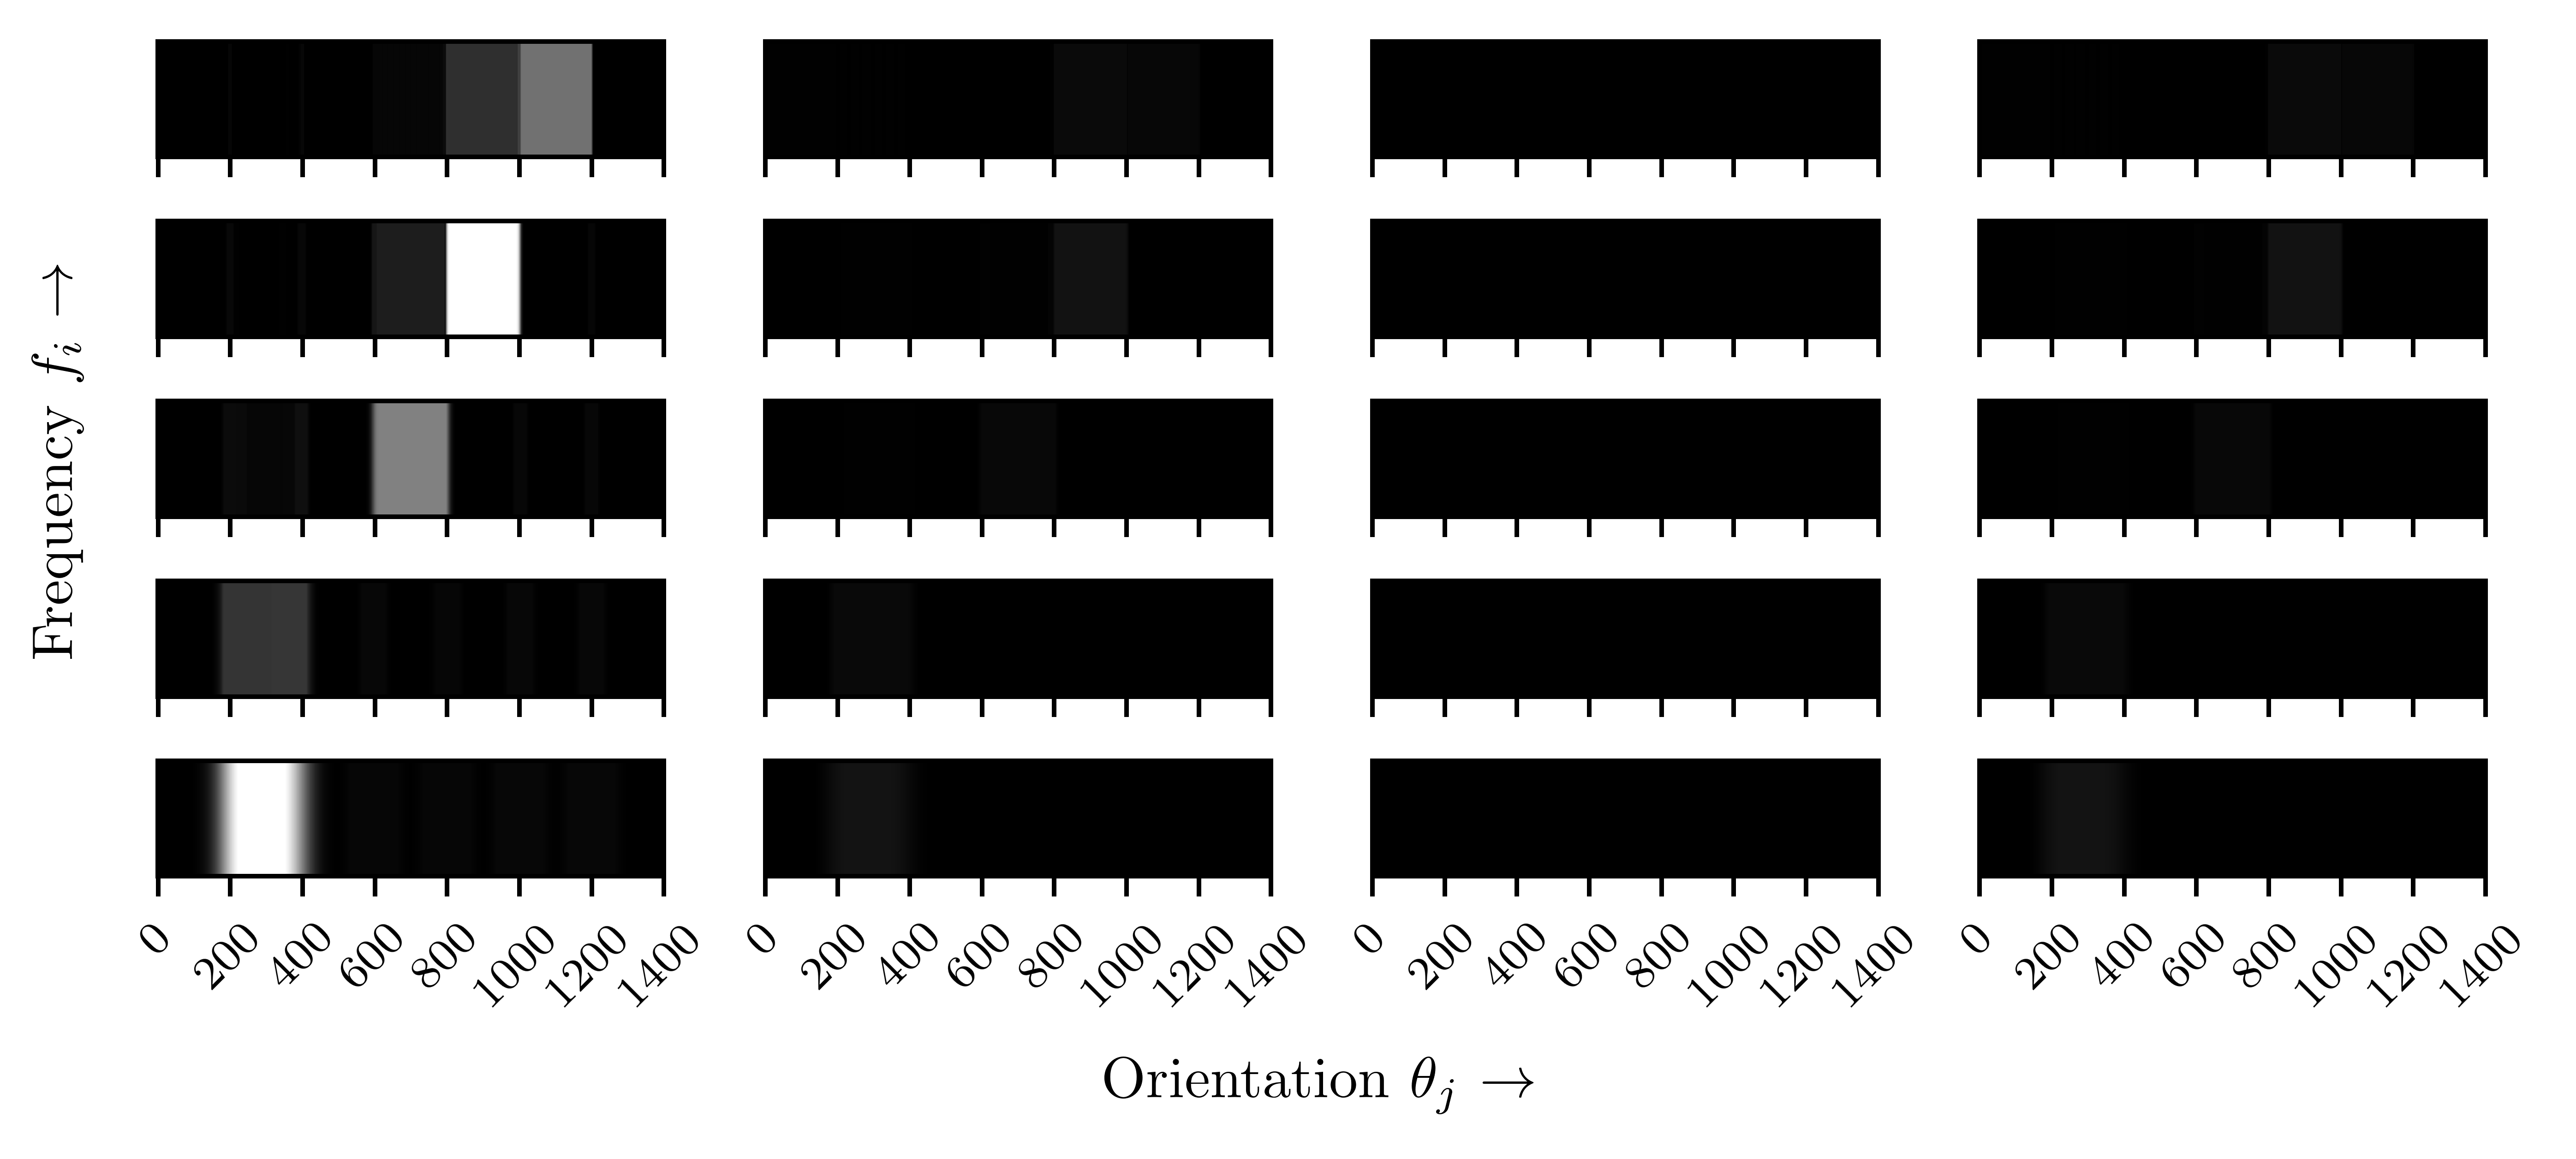
\includegraphics[width=\textwidth]{gabor_resp_ci_synthetic_opn}
        \caption{$\widetilde{e}_{\IM(C), f, \theta}(x,y)$}
        \label{fig:ci_gabor_energies_opn_smth} 
    \end{subfigure} 
    	    
    \caption{Gabor responses after morphological openning and Gaussian smoothing of the synthetic image. \captext{(a)} luminance channel responses, \captext{(b)} real part of chrominance channel responses, \captext{(c)} imaginary part of chrominance channel responses.}\label{fig:synthetic_img_gresponses_opn_smth}    
\end{figure}



%Taking for example the Gabor filter at frequency $f = 1/4$ (highest frequency on the image textures) and orientation $\theta = 0^\circ$ (vertical textures), the Gabor enrgy Eq. \eqref{eq:gabor_energy} obtained when applying the filter on the channels of the synthetic image is depicted by figure \ref{fig:synthetic_img_gresponse_00}. The result of convolution shows 
%
%\begin{figure}[!ht]
%    \centering
%    \begin{subfigure}[b]{\textwidth}
%        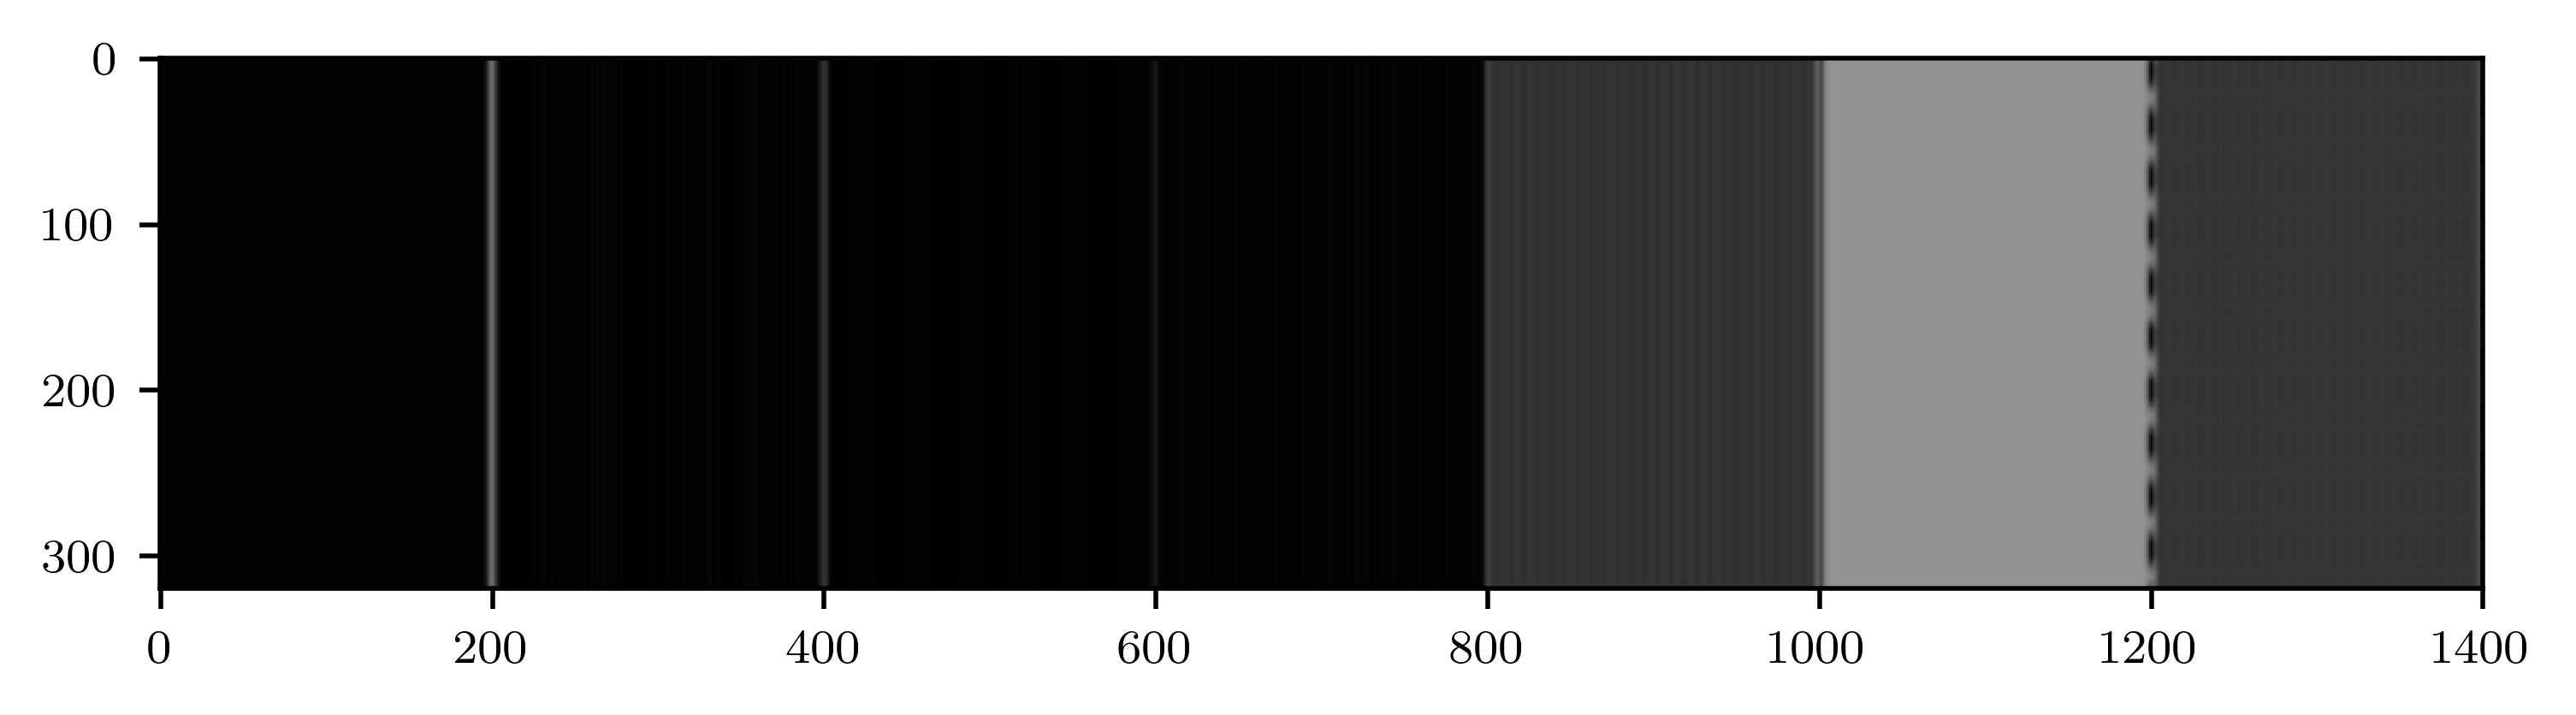
\includegraphics[width=\textwidth]{gabor_resp_lum_synthetic_00}
%        \caption{$e_{L, f, \theta}(x,y)$}
%    \end{subfigure} \\    
%    \begin{subfigure}[b]{\textwidth}
%    	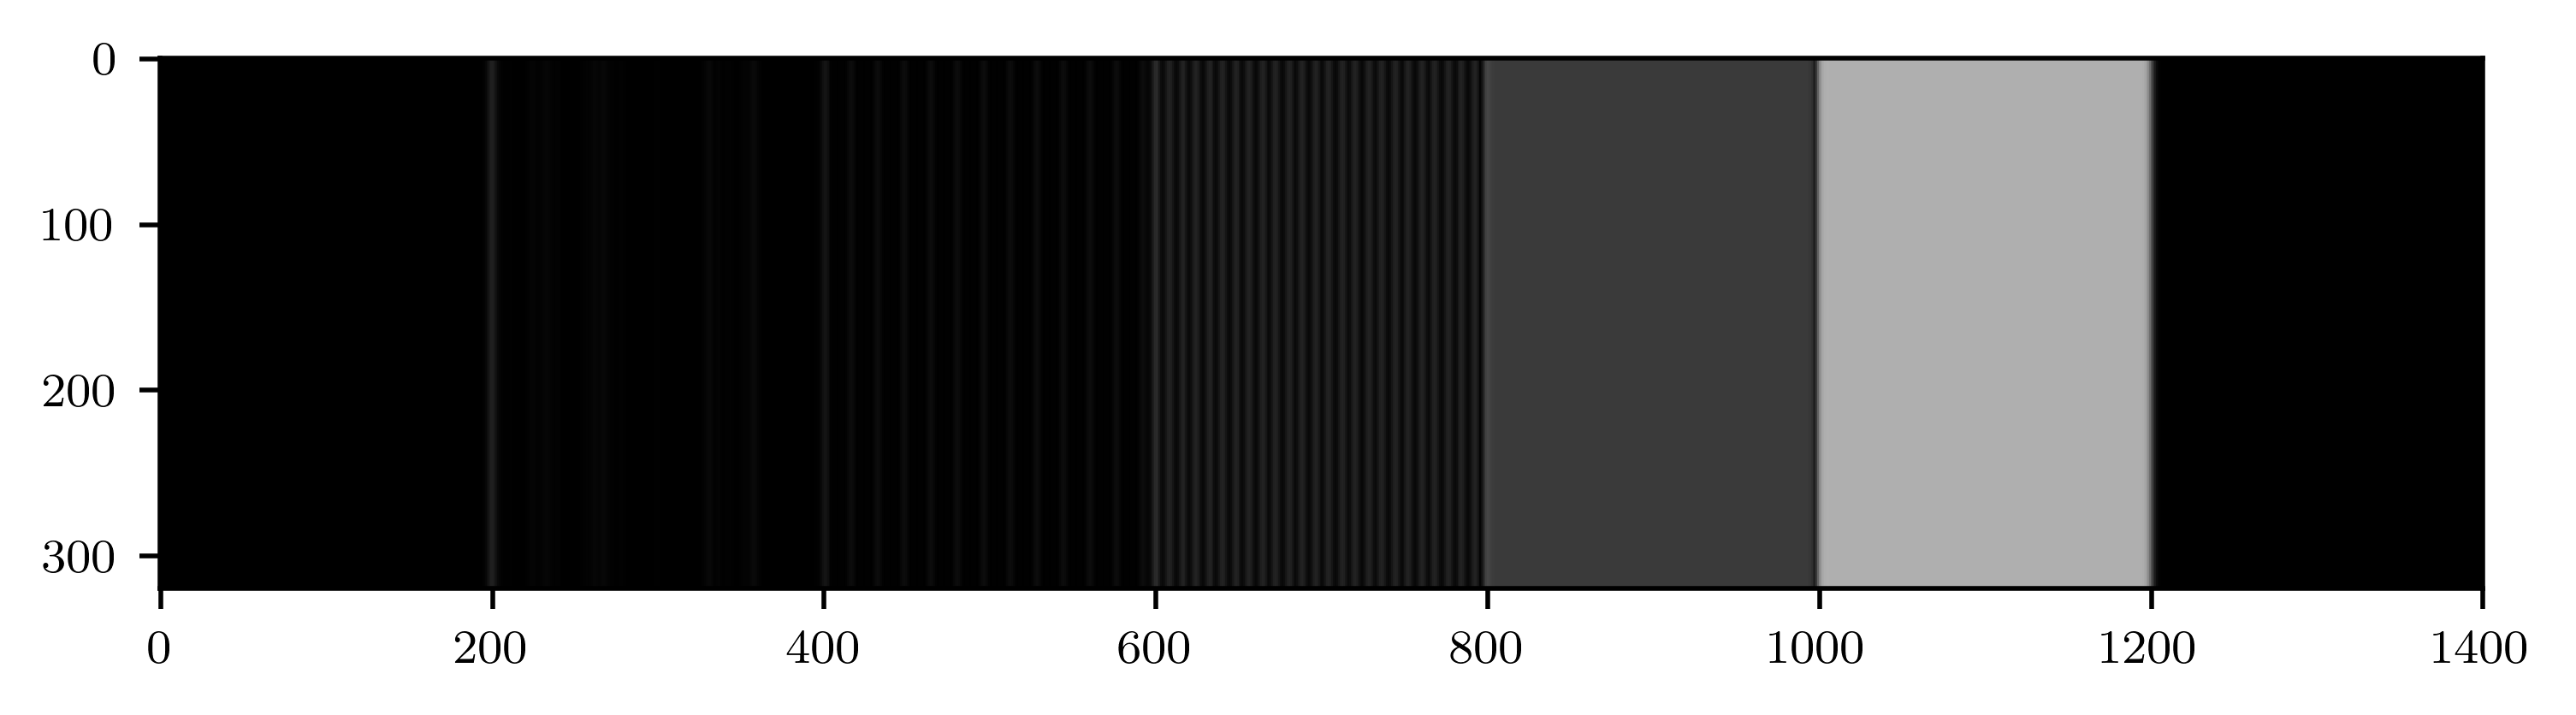
\includegraphics[width=\textwidth]{gabor_resp_cr_synthetic_00}
%        \caption{$e_{\RE(C), f, \theta}(x,y)$}
%    \end{subfigure} \\    	
%    \begin{subfigure}[b]{\textwidth}
%        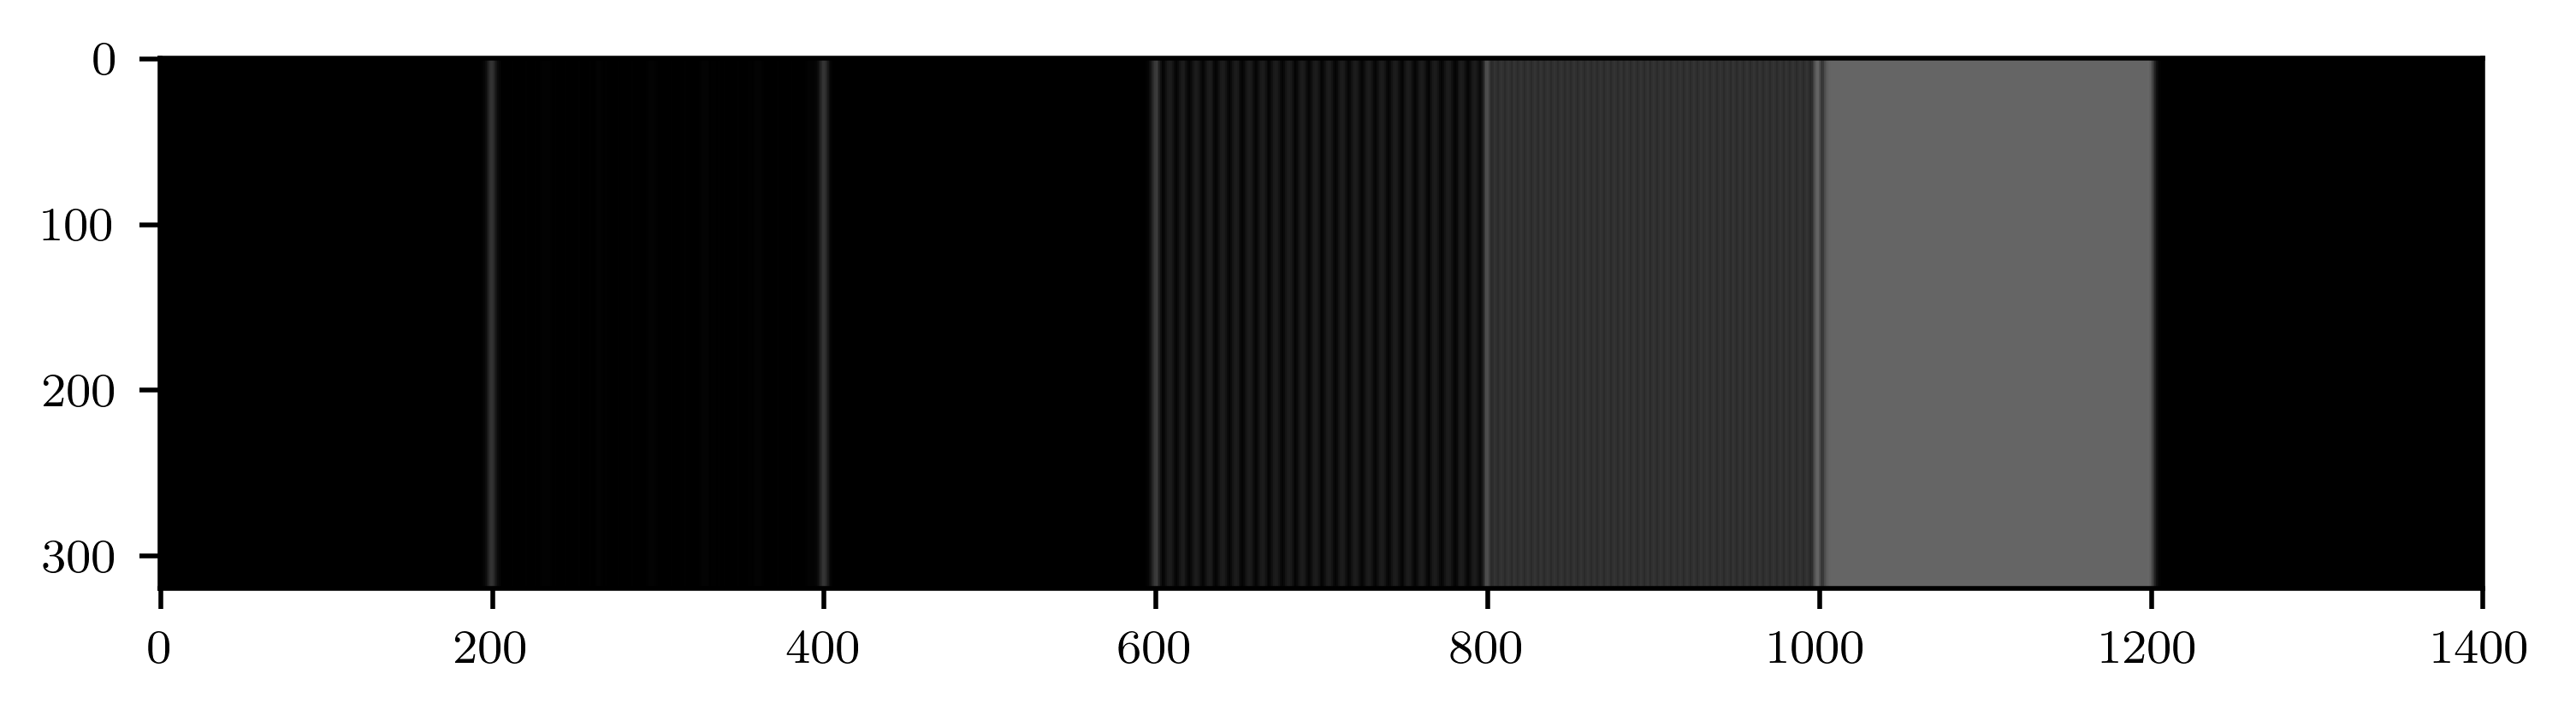
\includegraphics[width=\textwidth]{gabor_resp_ci_synthetic_00}
%        \caption{$e_{\IM(C), f, \theta}(x,y)$}
%    \end{subfigure} 
%    \caption{Raw Gabor energy obtained a $f=1/4$ and $\theta=0^\circ$.}\label{fig:synthetic_img_gresponse_00}    
%\end{figure}
%

% 	    
%
%
%\begin{figure}[!ht]
%    \centering
%    \begin{subfigure}[b]{\textwidth}
%        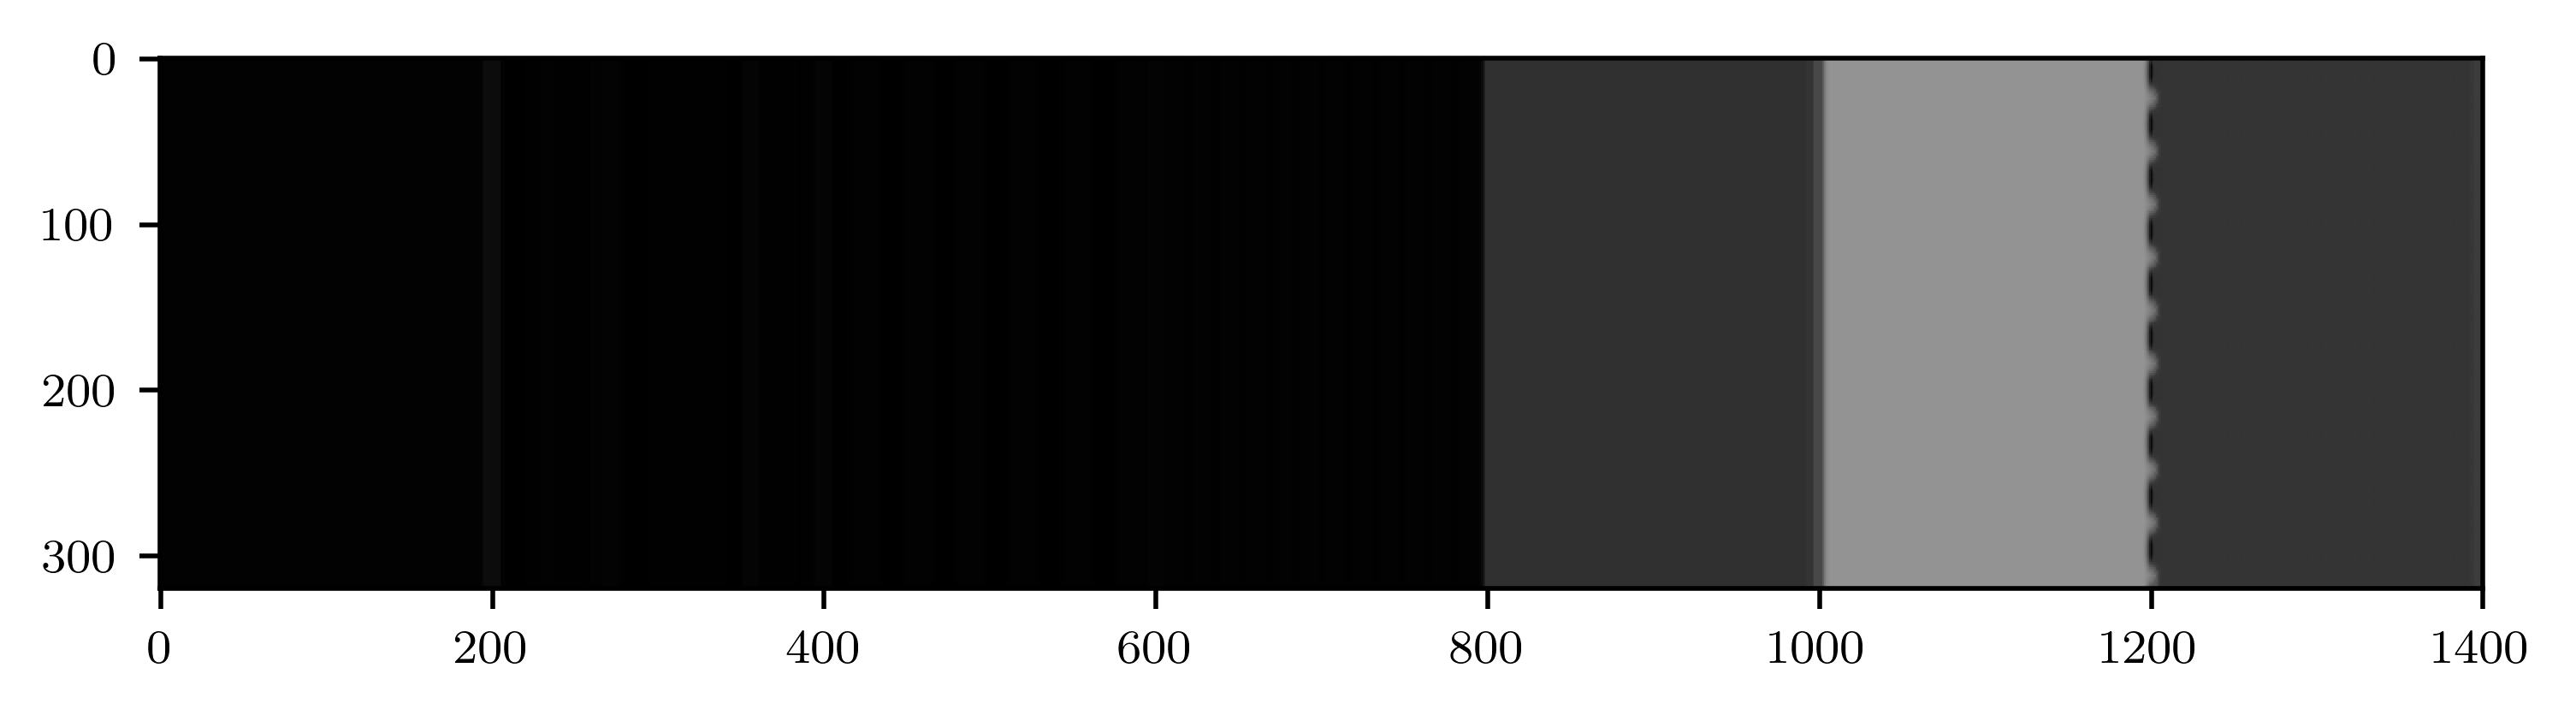
\includegraphics[width=\textwidth]{gabor_resp_lum_synthetic_00_opn}
%        \caption{$\widehat{e}_{L, f, \theta}(x,y)$}
%    \end{subfigure} \\    
%    \begin{subfigure}[b]{\textwidth}
%    	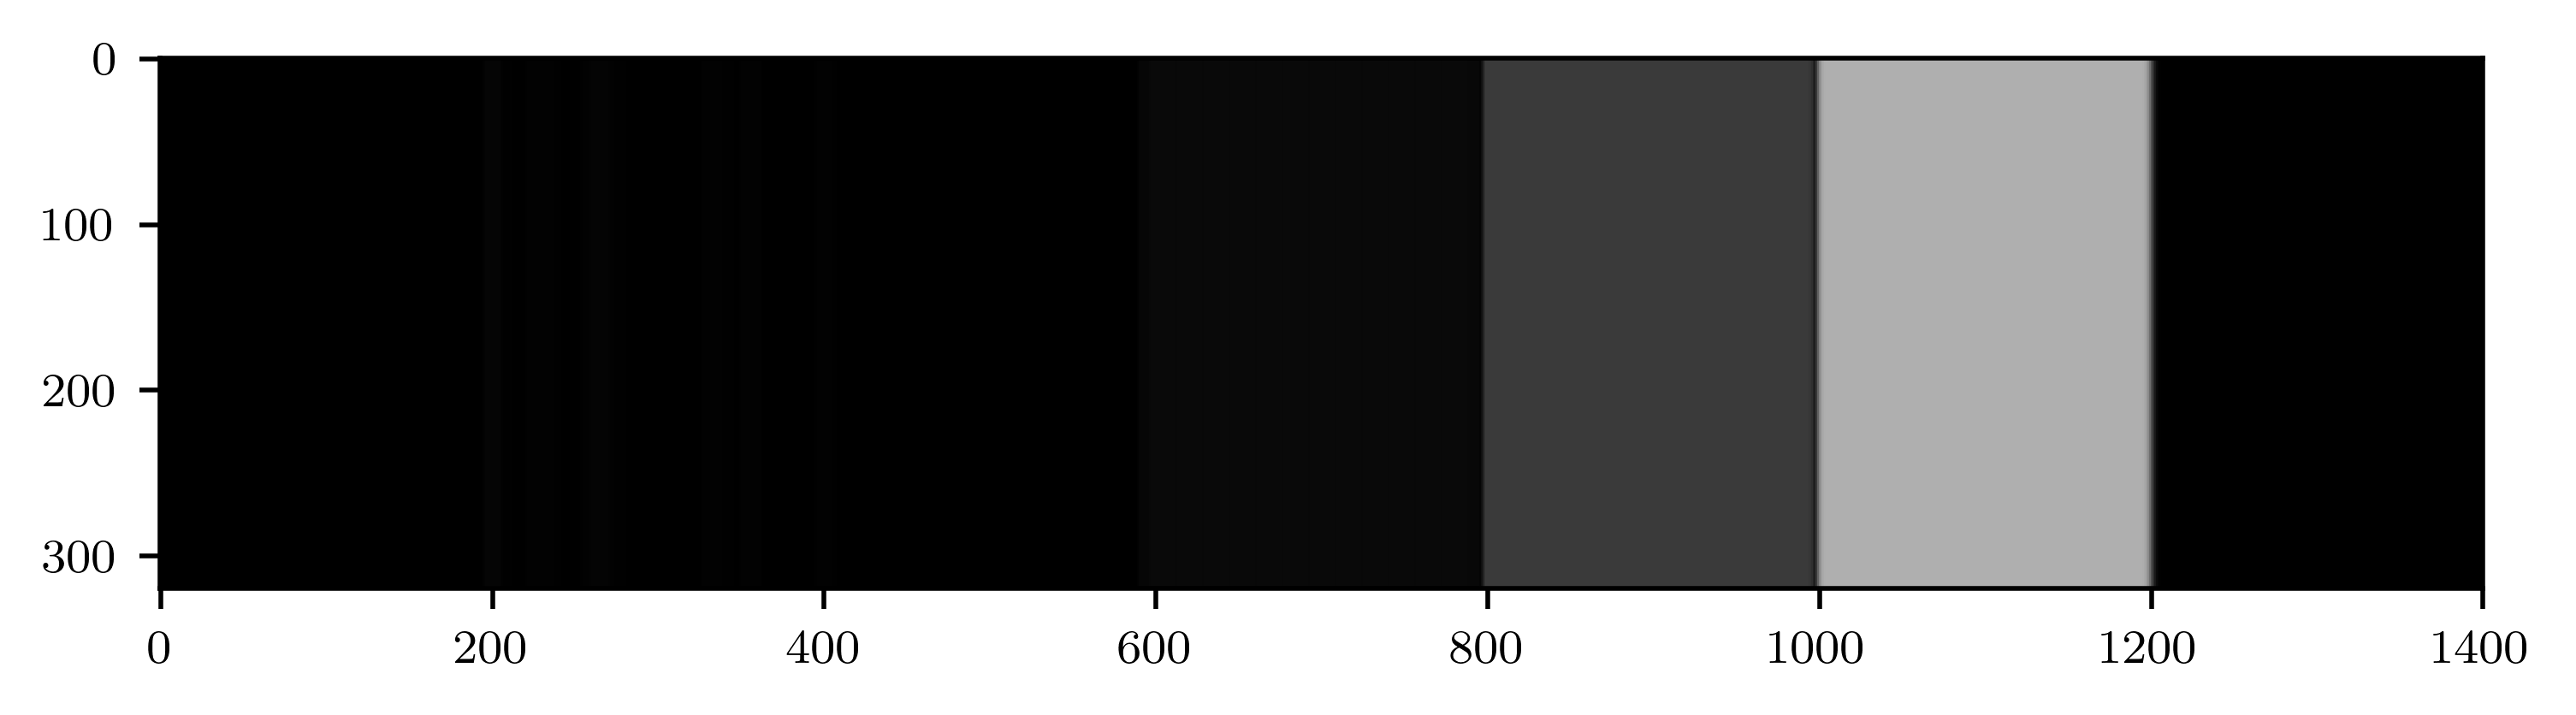
\includegraphics[width=\textwidth]{gabor_resp_cr_synthetic_00_opn}
%        \caption{$\widehat{e}_{\RE(C), f, \theta}(x,y)$}
%    \end{subfigure} \\    	
%    \begin{subfigure}[b]{\textwidth}
%        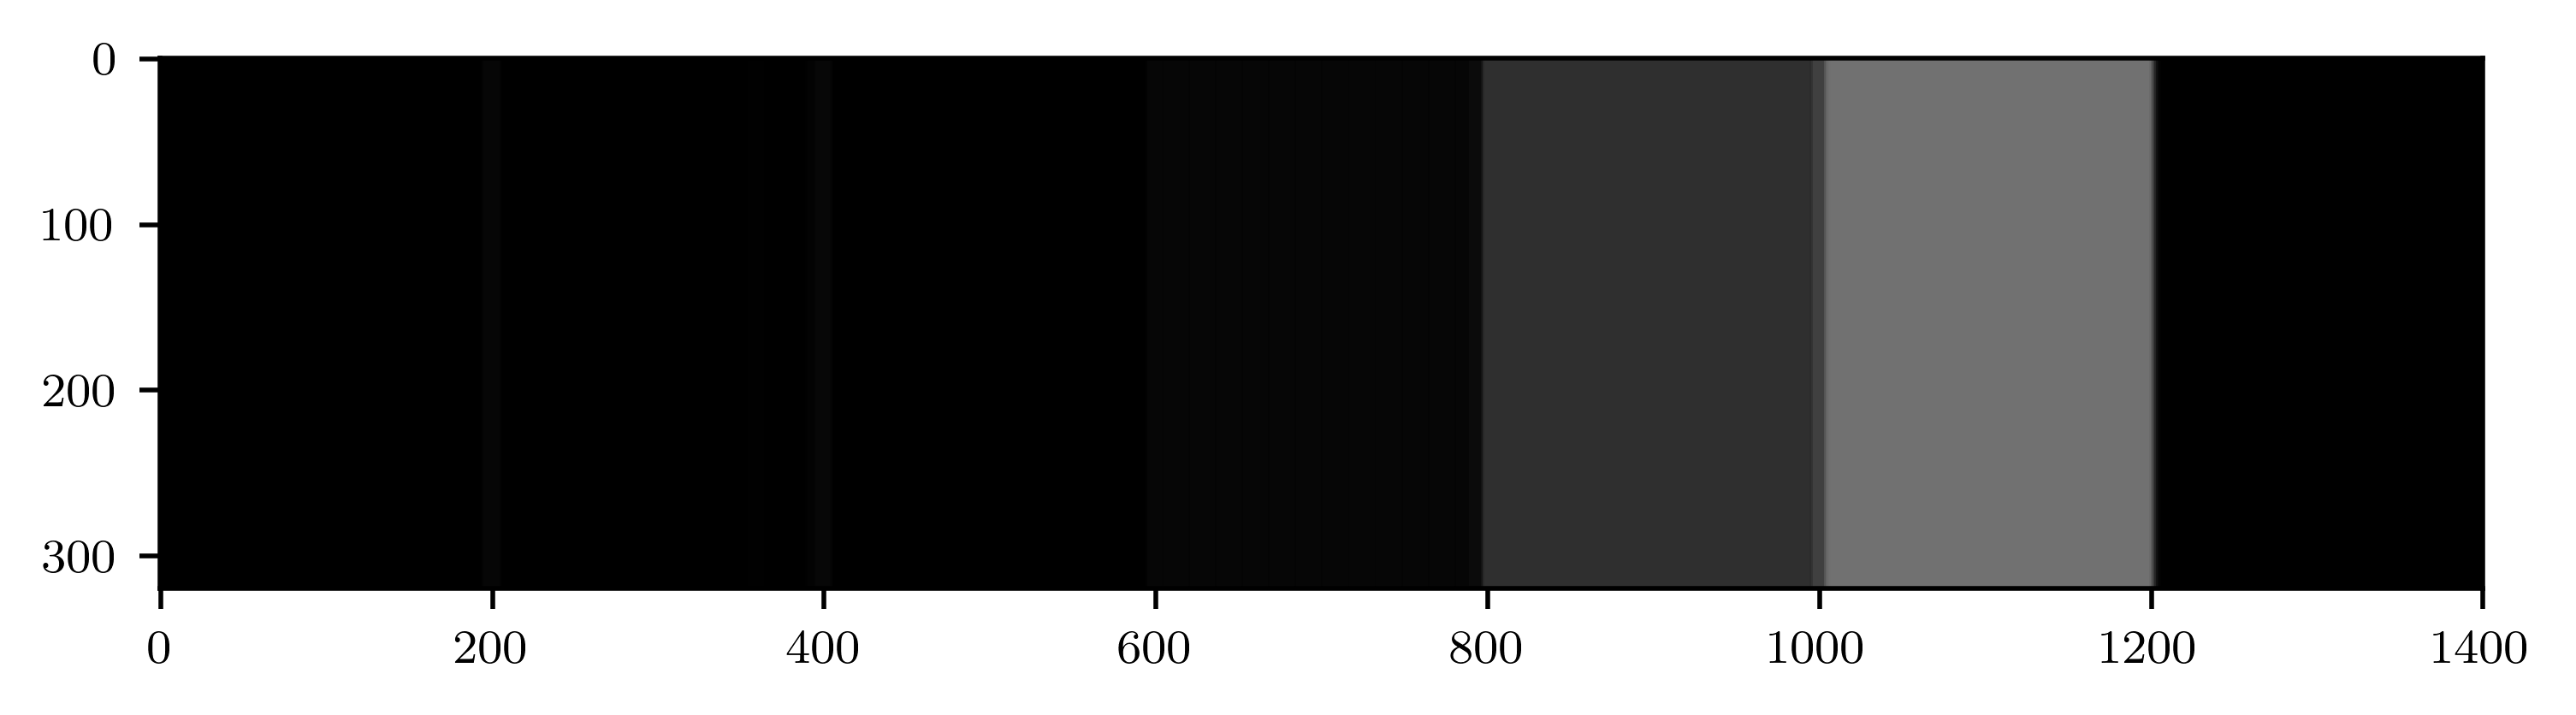
\includegraphics[width=\textwidth]{gabor_resp_ci_synthetic_00_opn}
%        \caption{$\widehat{e}_{\IM(C), f, \theta}(x,y)$}
%    \end{subfigure} 
%    	    
%    \caption{Gabor response obtained a $f=1/4$ and $\theta=0^\circ$ after morphological openning.}\label{fig:synthetic_img_gresponse_00_opn}    
%\end{figure}
%
%
%
%
%\begin{figure}[!ht]
%    \centering
%    \begin{subfigure}[b]{\textwidth}
%        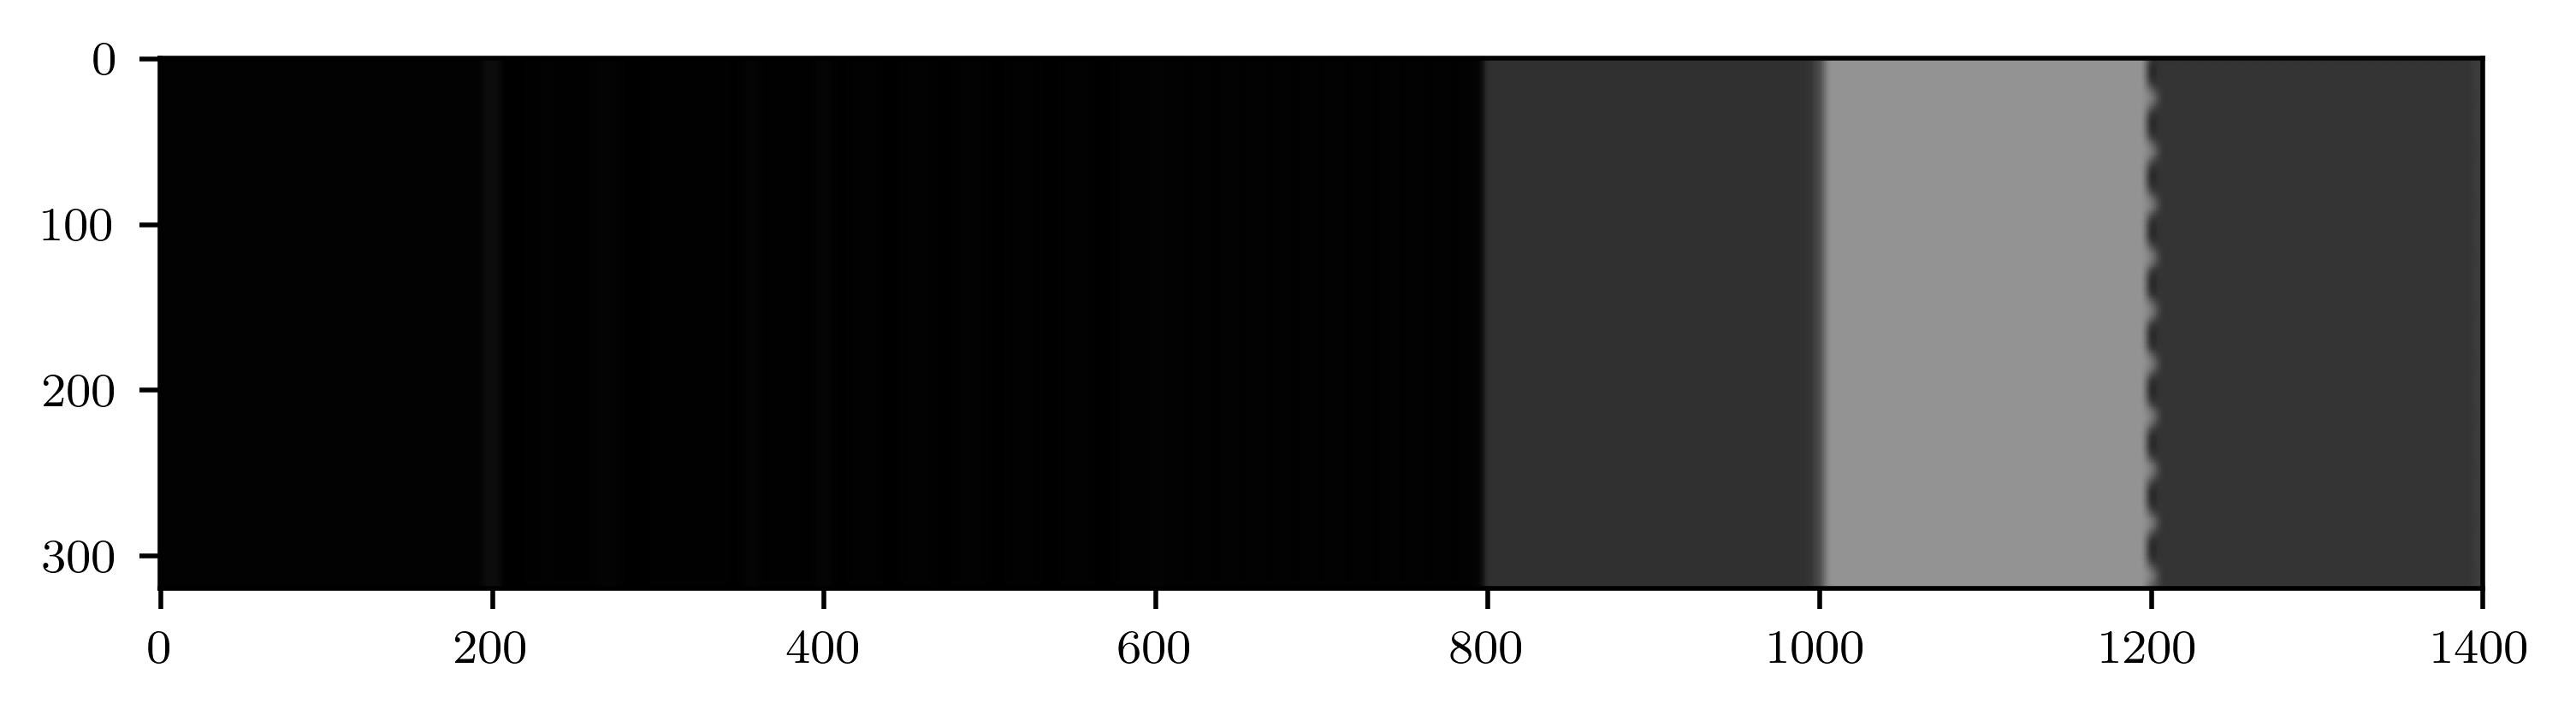
\includegraphics[width=\textwidth]{gabor_resp_lum_synthetic_00_opn_smth}
%        \caption{$\widetilde{e}_{L, f, \theta}(x,y)$}
%    \end{subfigure} \\    
%    \begin{subfigure}[b]{\textwidth}
%    	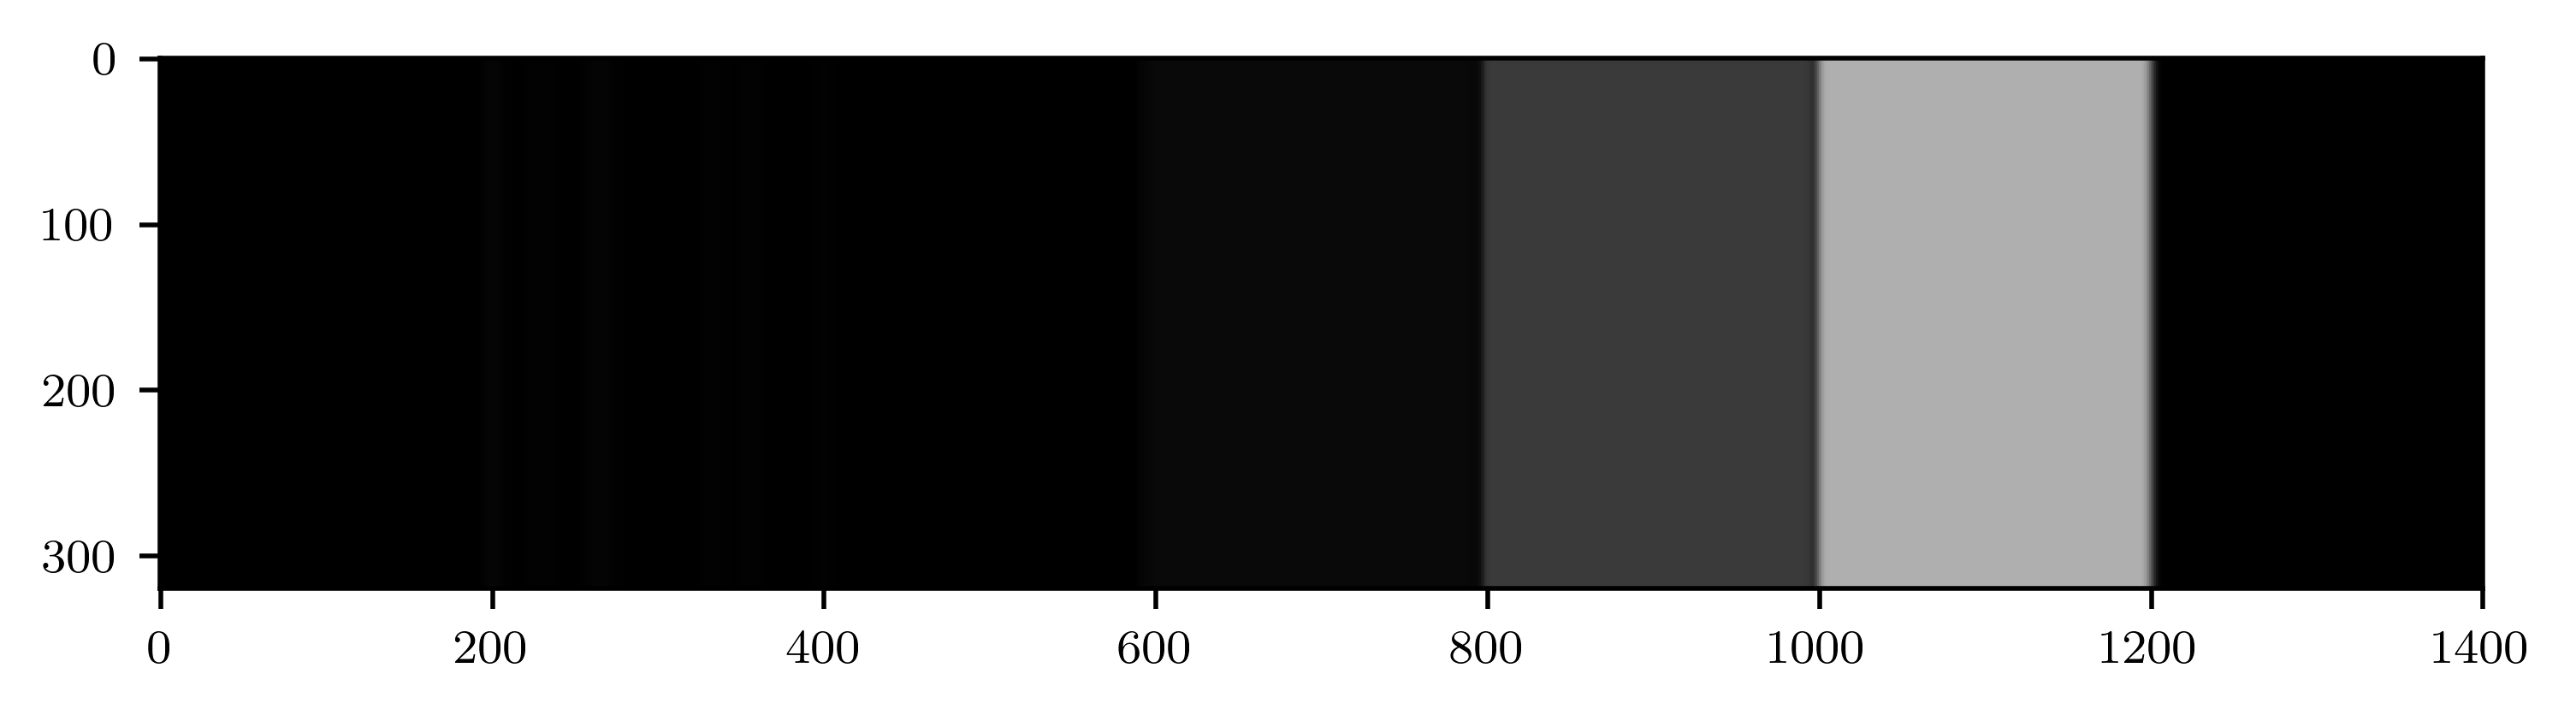
\includegraphics[width=\textwidth]{gabor_resp_cr_synthetic_00_opn_smth}
%        \caption{$\widetilde{e}_{\RE(C), f, \theta}(x,y)$}
%    \end{subfigure} \\    	
%    \begin{subfigure}[b]{\textwidth}
%        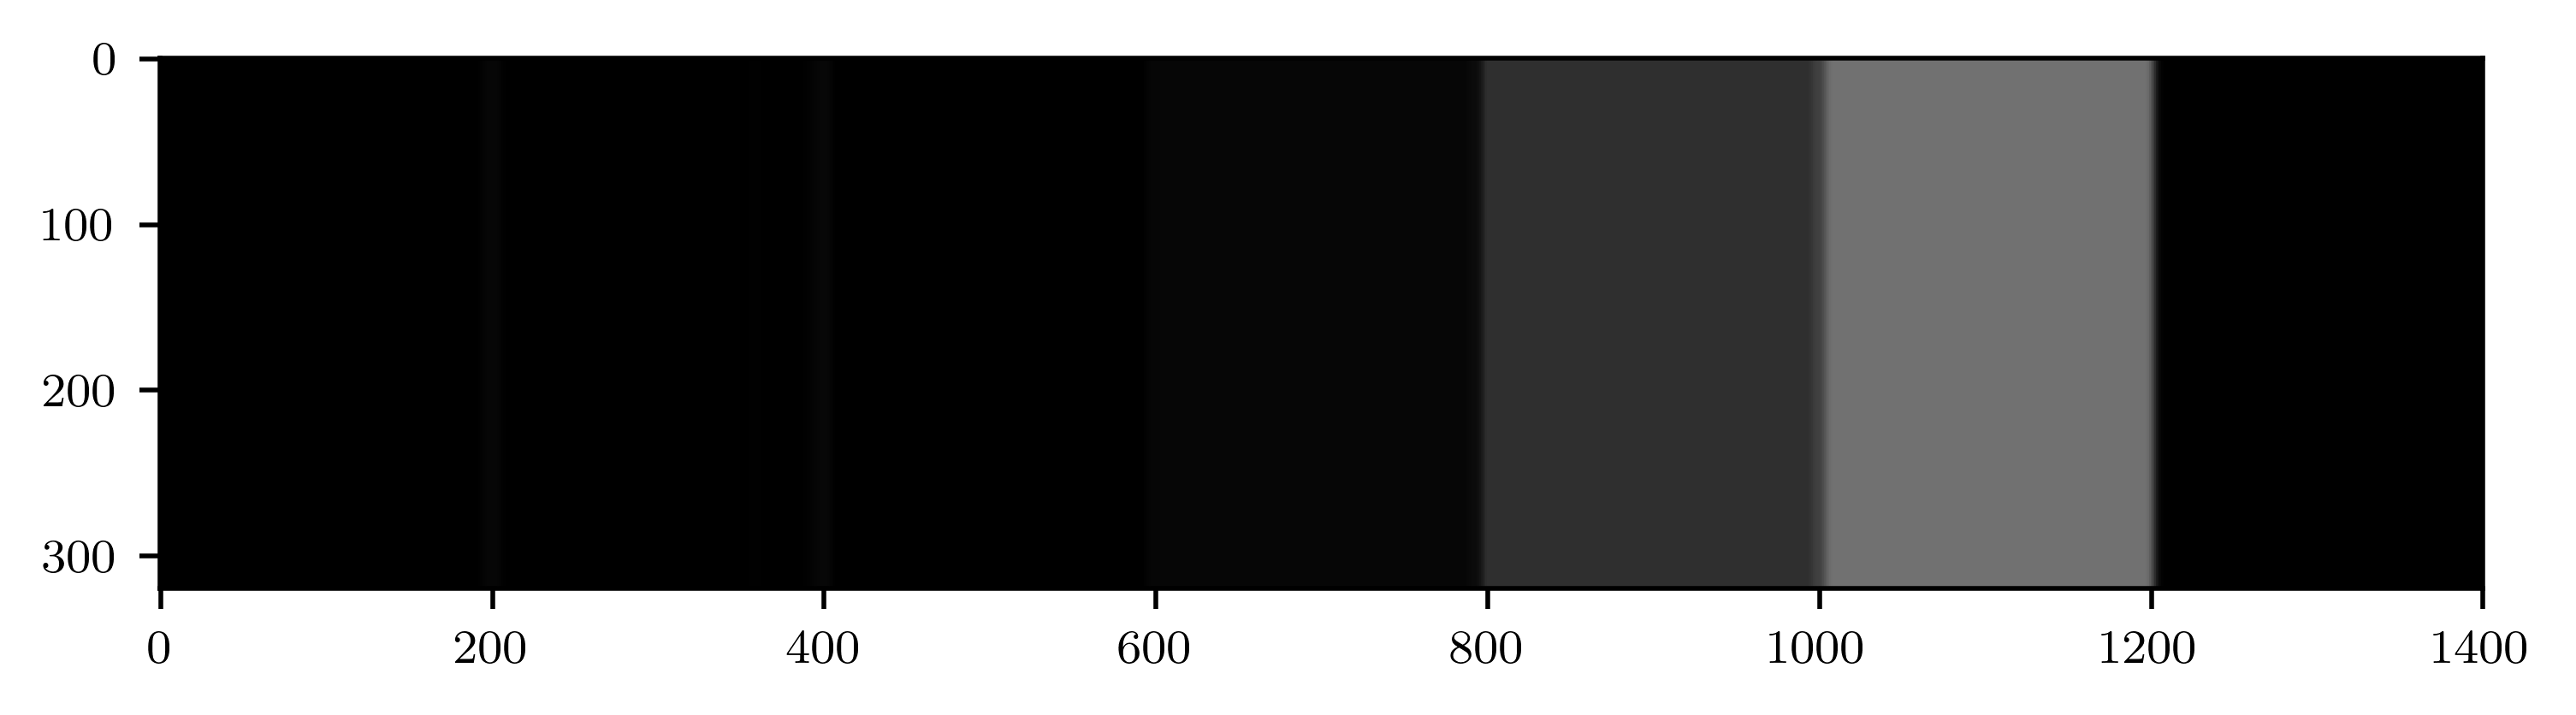
\includegraphics[width=\textwidth]{gabor_resp_ci_synthetic_00_opn_smth}
%        \caption{$\widetilde{e}_{\IM(C), f, \theta}(x,y)$}
%    \end{subfigure} 
%    	    
%    \caption{Gabor response obtained a $f=1/4$ and $\theta=0^\circ$ after morphological openning and Gaussian smoothing.}\label{fig:synthetic_img_gresponse_00_opn_smth}    
%\end{figure}



\section{Gabor Filter-based Feature Space Validation}

In this section, we integrate the feature space obtained with Gabor filters within a clustering framework. We hypothesize that if the color/texture features represent the variety of information in the images (synthetic and natural), we can obtain a consistent segmentation with this perceptual information. We then use the segmentation results to qualitatively and quantitatively evaluate our Gabor feature space.

Before clustering, we adapt the feature space to prepare it for the clustering methods.

\paragraph{Data organization}
The feature space 
\begin{equation}\label{eq:feature_space_clustering}
	X(x,y) = \widetilde{e}_{i, f, \theta}(x,y)
\end{equation}
is a log-polar space given the logarithmic scale of the $N$ frequencies and the $N$ orientations of the Gabor filter bank. Then, the feature space is composed of $3 \times M \times N$ Gabor responses, where the constant $3$ corresponds to the number of channels of the luminance-chrominance color space. We arrange the data to obtain a two-dimensional array of size $P \times D$, where $P= H\times W$  is the number of samples or pixels and $D =3 \times M \times N$ in the number of features or dimensions of the data.

\paragraph{Spatial information integration}
Gabor's color and texture features do not include spatial information. We enter such information by adding two more dimensions to the feature space $X$. These two features are the positional coordinates $(x, y)$ of each pixel in the image. 

\paragraph{Data standardization}
We standardize each feature $D$ of the $X$ matrix so that it has a mean of zero and a constant variance. We perform this operation to avoid the dominance of some features over others due to numerical differences of units of magnitude.

\paragraph{Dimensionality reduction}
We reduce the feature space's dimensions from $D =3 \times M \times N$ to $5$ using the linear transformation technique of principal component analysis (PCA). With the PCA we identify patterns in the feature space based on the correlation between features. We choose 5 as the new subspace dimension based on the idea that three of these dimensions contain Gabor's color and texture information and the remaining two dimensions contain the spatial information. In addition, a low number of dimensions speeds up the calculation of clustering algorithms.

\subsection{Qualitative Evaluation}
We qualitatively validate the spectral decomposition of images based on Gabor filters for the generation of color texture features first, in fully controlled conditions using the synthetic image and later, with a semi-controlled set up using handmade texture mosaics.

In both cases, we use the k-means algorithm as a clustering method on the feature space $X$ setting the number of clusters manually. The grouping technique acts as a segmentation method, with which we validate our methodology.

\subsubsection{Synthetic image segmentation}
Looking at the synthetic image (Fig. \ref{fig:synthetic_color_texture_image}),  there are several coherent ways for a human observer to segment it. The two most apparent possibilities are to segment the image into 7 clusters, where each cluster represents a region of the image and; segment the image only into 2 clusters, where one cluster groups the regions with texture and the other the flat region. 

We apply these conditions to set the clusters' number of the k-means algorithm $k = 7$ and $k = 2$ ,  and obtain a segmentation of the synthetic image coherent with the human perception. The segmentation results are depicted in figure  \ref{fig:kmeans_segms_synthetic_img}. These segmentation results show that the Gabor multi-spectral analysis captures well the color and texture information. Also, the segmentation shows that both features (color and texture) are perceptually relevant in the image segmentation task.  

\begin{figure}[!ht]
    \centering
    \begin{subfigure}[b]{\textwidth}
        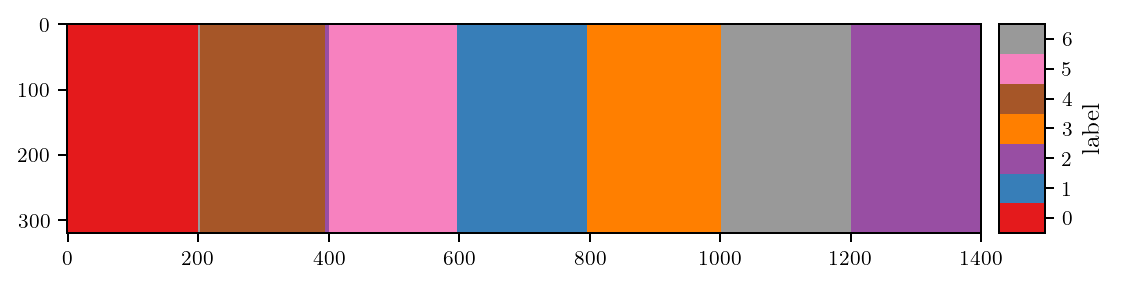
\includegraphics[width=\textwidth]{kmeans_7segms_synthetic}
        \caption{7 clusters segmentation}
    \end{subfigure} \\    
    \begin{subfigure}[b]{\textwidth}
    	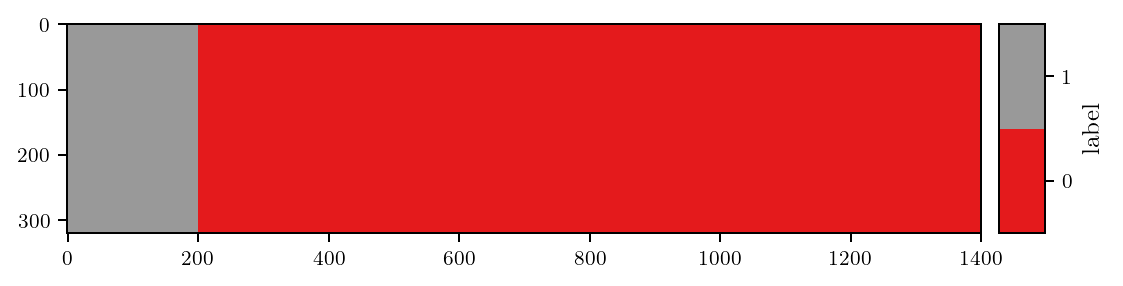
\includegraphics[width=\textwidth]{kmeans_2segms_synthetic}
        \caption{2 clusters segmentation}
    \end{subfigure} 
        	    
    \caption{Synthetic image k-means segmentation results.}\label{fig:kmeans_segms_synthetic_img}    
\end{figure}

\subsubsection{DTD mosaic image segmentation}
We go a step further and test our feature space under slightly more complex conditions; we created a series of color texture mosaics using images from the Describable Textures Dataset (DTD) \citep{Cimpoi.Maji.ea:CVPR:2014} as a base. The DTD is a collection of homogeneous nature textures with 47 annotated classes. To create the mosaics, we take 5 images of the same (or similar ) class and put them together in a collage. The five classes we take the images are \textit{lined-banded-zigzagged}, \textit{cracked}, \textit{braided}, \textit{dotted}, and \textit{striped-veined-scaly}. The texture collage we propose is relatively standard, with a circular patch in the center of the image that is superimposed on four square patches. 

We apply the clustering algorithm on each mosaic created, setting $ k = 5 $ clusters. The segmentation results are shown in figure \ref{fig:kmeans_segms_dtd_mosaics}. In this case, the clustering algorithm results are coherent with the input image; however, the segmentation's precision and quality are lower than in the case of the synthetic image. This result is mainly due to the complexity of the natural textures in the mosaics. 

\begin{figure}[!ht]
    \centering
    \begin{subfigure}[b]{0.19\textwidth}
        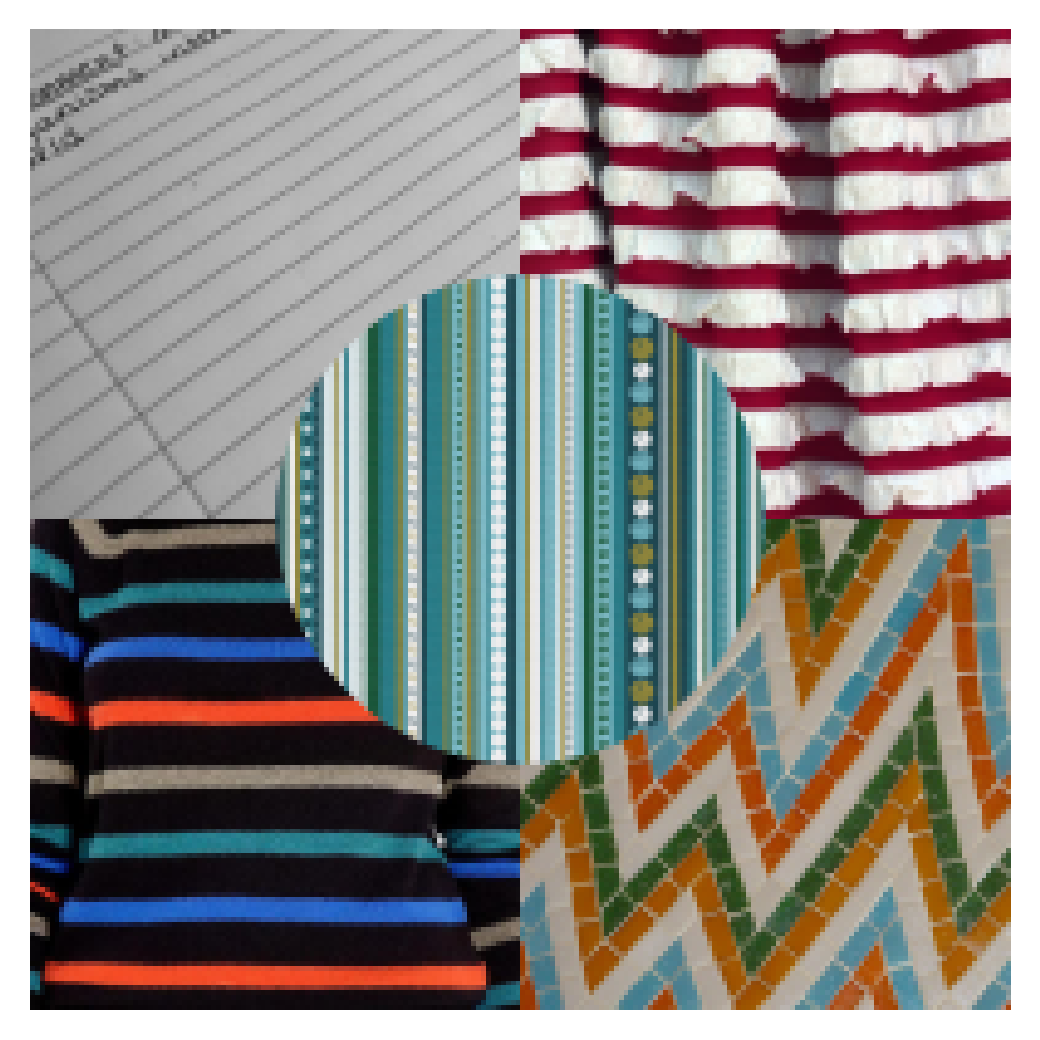
\includegraphics[width=\textwidth]{mosaic_dtd1}
    \end{subfigure} 
    \begin{subfigure}[b]{0.19\textwidth}
    	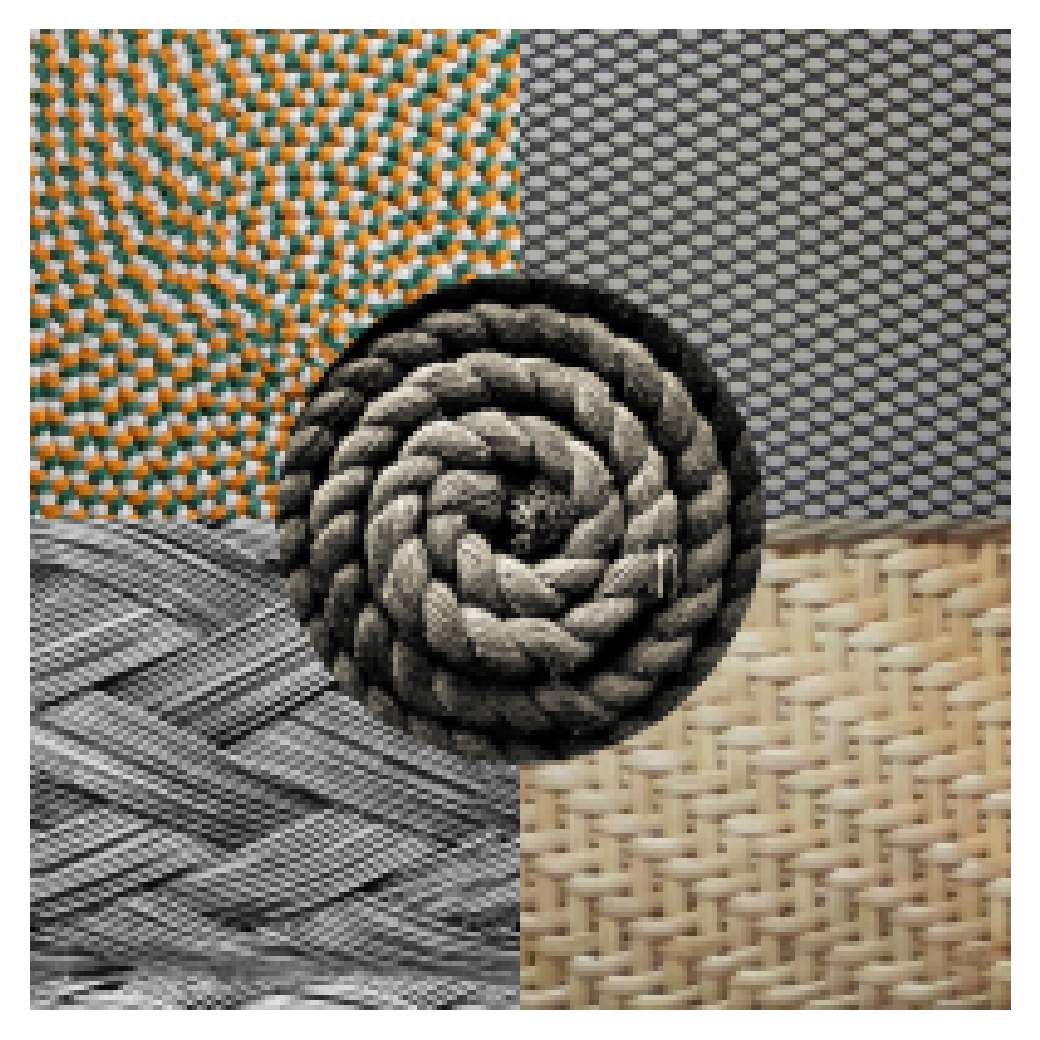
\includegraphics[width=\textwidth]{mosaic_dtd2}
    \end{subfigure}     
    \begin{subfigure}[b]{0.19\textwidth}
        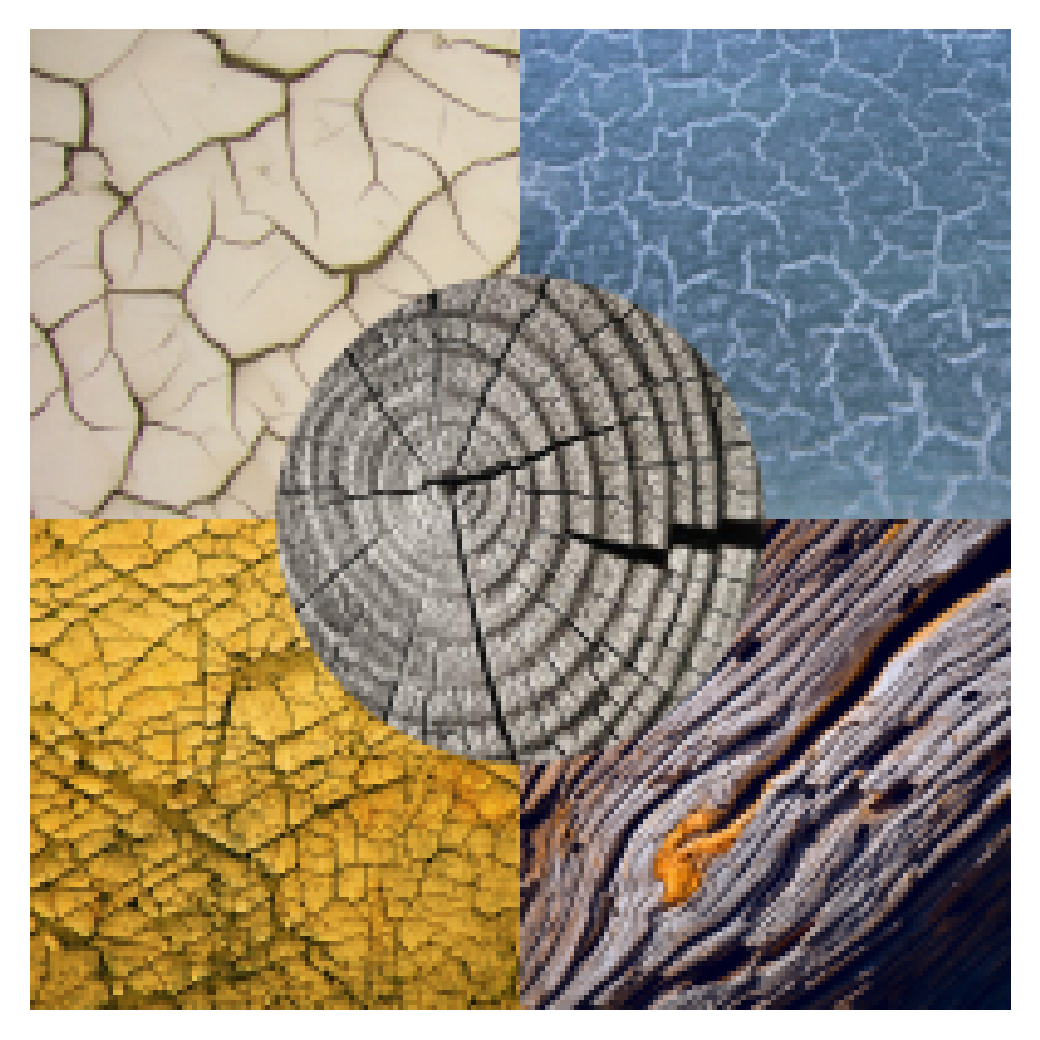
\includegraphics[width=\textwidth]{mosaic_dtd3}
    \end{subfigure}
    \begin{subfigure}[b]{0.19\textwidth}
    	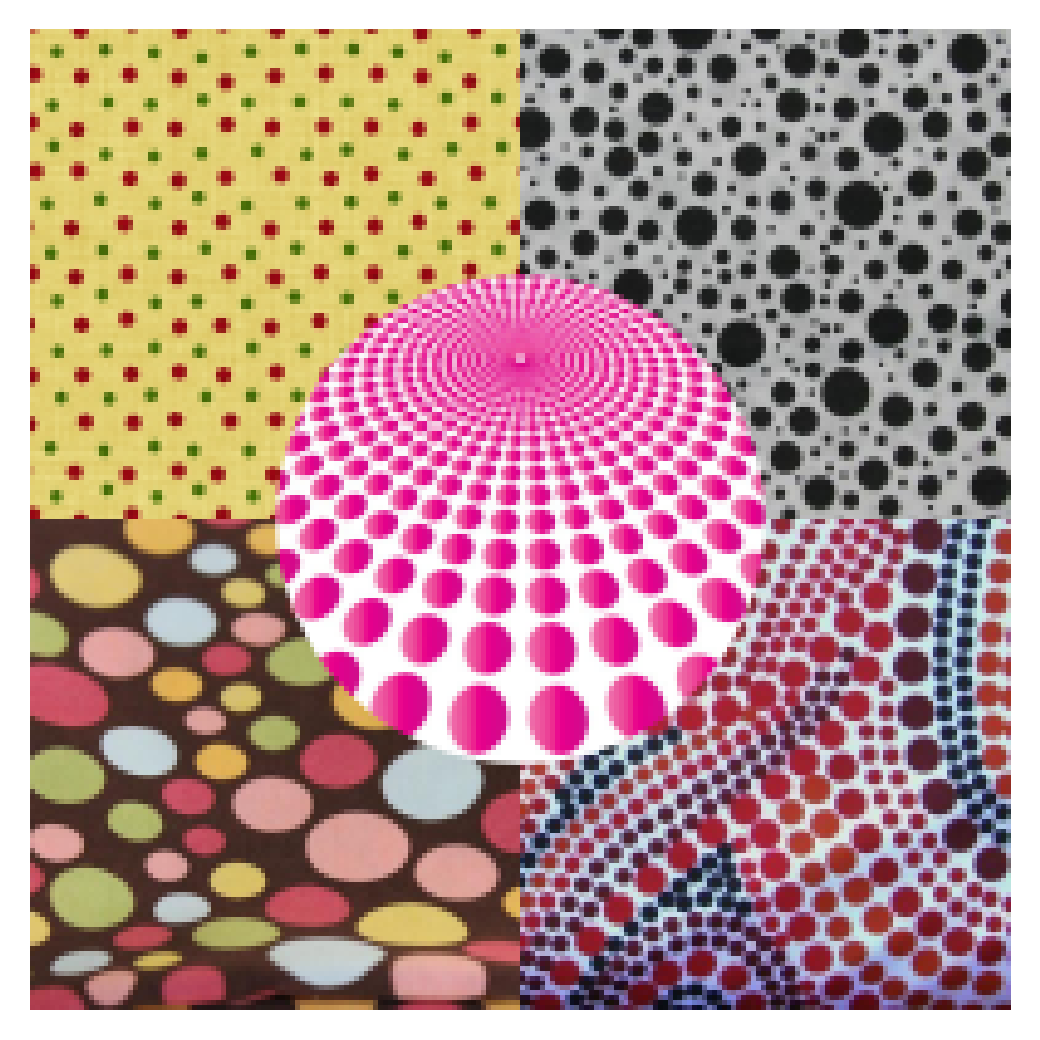
\includegraphics[width=\textwidth]{mosaic_dtd4}
    \end{subfigure}    
    \begin{subfigure}[b]{0.19\textwidth}
        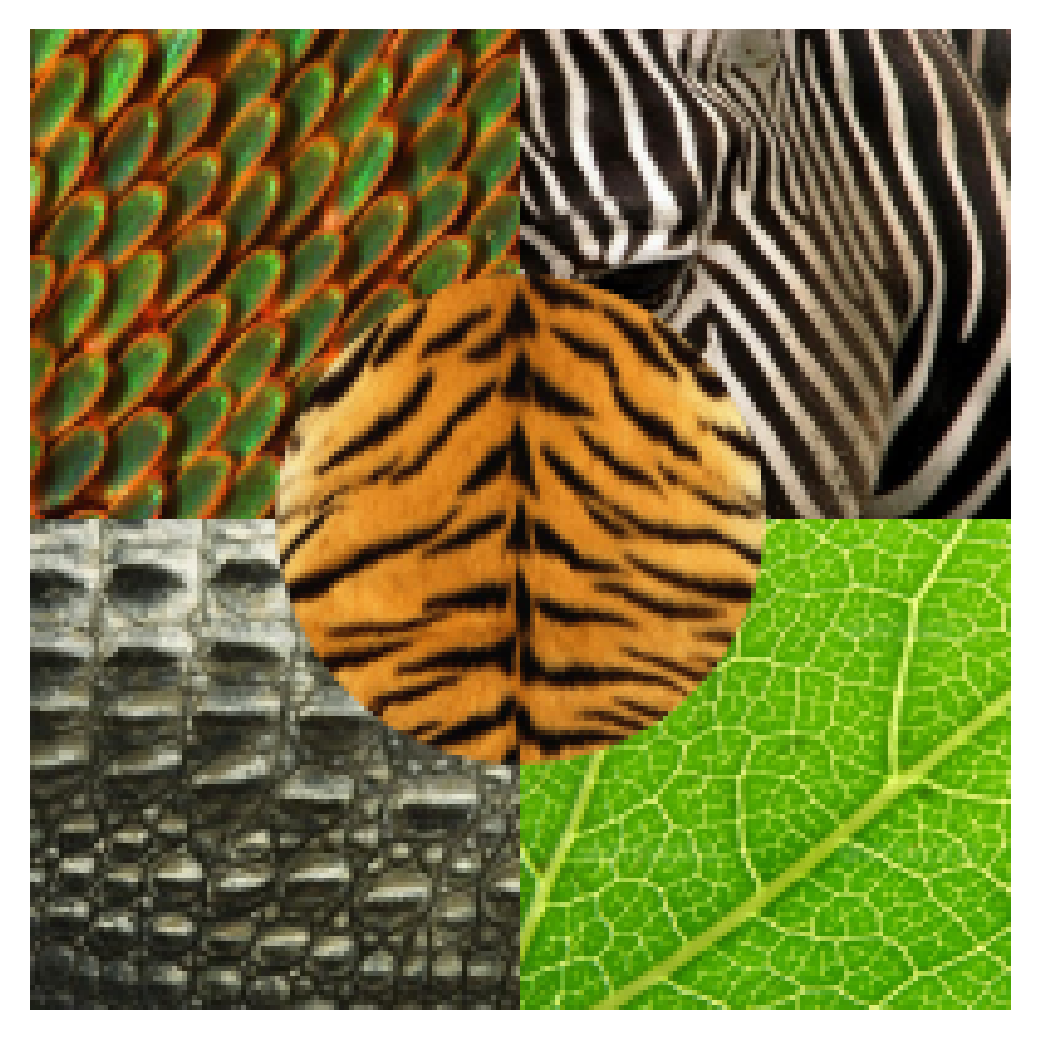
\includegraphics[width=\textwidth]{mosaic_dtd5}
    \end{subfigure} \\ [2ex]
    
    \begin{subfigure}[b]{0.19\textwidth}
    	
\includegraphics[width=\textwidth]{mosaic_dtd1_kmeans_segms}
        \caption{}
    \end{subfigure}     
    \begin{subfigure}[b]{0.19\textwidth}
        
\includegraphics[width=\textwidth]{mosaic_dtd2_kmeans_segms}
        \caption{}
    \end{subfigure} 
    \begin{subfigure}[b]{0.19\textwidth}
    	
\includegraphics[width=\textwidth]{mosaic_dtd3_kmeans_segms}
        \caption{}
    \end{subfigure}     
    \begin{subfigure}[b]{0.19\textwidth}
        
\includegraphics[width=\textwidth]{mosaic_dtd4_kmeans_segms}
        \caption{}
    \end{subfigure}
    \begin{subfigure}[b]{0.19\textwidth}
    	
\includegraphics[width=\textwidth]{mosaic_dtd5_kmeans_segms}
        \caption{}
    \end{subfigure} 
        	    
    \caption{DTD mosaics k-means segmentation results.}\label{fig:kmeans_segms_dtd_mosaics}    
\end{figure}


\subsection{Quantitative Evaluation}\label{subsec:quantitative_evaluation}

We also quantitatively evaluate the quality of the feature space developed in this chapter. For this, we use a database of natural images that have a ground truth generated by humans. The database and its characteristics are described below.

\subsubsection{Berkely Segmentation Image Data Set}
The Berkely Database for Segmentation (BSDS) is one of the gold standards for segmentation results \citep{Martin.Fowlkes.ea:ICCV:2001}. The BSDS comprises images from the Corel database selected under a simple criterion: choose images of complex and natural scenes containing at least one distinguishable object. Under this criteria, selected images contain multiple cues for human segmentation, for example, low-level cues such as coherence of brightness, texture, color, and contour continuity; mid-level cues such as symmetry, convexity, and area of the regions; as well as high-level cues based on the semantics of the image objects.

There are two versions of this database. The first one (BSDS300) contains 300 images, while the second (BSDS500) contains 500 images. Each image in the database contains between 5 and 11 human-made segmentations. The instruction given to the observers to naturally break the scene is simple:
\begin{displayquote}
Divide each image into pieces, where each piece represents a distinguished thing in the image. It is important that all of the pieces have approximately equal importance. The number of things in each image is up to you. Something between 2 and 30 should be reasonable for any of our images \citep{Martin.Fowlkes.ea:ICCV:2001}.
\end{displayquote}
Following these instructions, most segmentations meet the criterion of the number of segments; however, we can also find exceptions with more than 50 segmented things.

Finally, both databases (BSDS300 and BSDS500) contain segmentations of gray level and color images. Since in this chapter we analyze the color textures, we mainly use the BSDS500 color images with their respective segmentations to evaluate our segmentation results. Figure 3 shows some examples of images from the BSDS500 and the segmentations produced by different humans.

\subsubsection{Scores}
We use the human-generated segmentations of the BSDS500 as ground truth (GT), applying the precision-recall framework of \cite{Martin.Fowlkes.ea:PAMI:2004}. The precision is the fraction of detections that are true positives rather than false positives, while the recall is the fraction of true positives that are detected rather than missed. This evaluation framework is generally applied to evaluate contour detection algorithms. Therefore, applied in the image segmentation task, the framework involves evaluating the boundaries of the segmentation resulting regions, considering the detected boundaries pixels as a two-classes classification problem (contour and non-contour pixels). Under this configuration, precision is translated as the number of pixels correctly labeled as belonging to the contour class (true positives) divided by the total number of pixels labeled as contours (the sum of true positives and false positives). The recall in this context is defined as the number of true positives divided by the sum of true positives and the pixels which were not labeled as contours but should have been (false negatives). The following mathematical expressions define the precision and the recall.

\begin{equation}\label{eq:precision_score}
    \text{precision} = \frac{tp}{tp+fp}
\end{equation}

\begin{equation}\label{eq:recall_score}
    \text{recall} = \frac{tp}{tp+fn}
\end{equation}

A simple metric that captures the trade-off between precision and recall is the f-measure, which is defined as the harmonic mean between the two scores.

\begin{equation}\label{eq:f_score}
    \text{F-measure} = \frac{2 \times \text{precision}\times\text{recall}}{\text{precision} + \text{recall}}
\end{equation}


\subsubsection{Experiments set up}

For the numerical evaluation, we perform the segmentation of the BSDS500 images using different clustering algorithms. In addition, we perform the segmentation in the feature space obtained with different luminance-chrominance color spaces, in particular those derived from the LAB, HSL, and HSV spaces. This series of experiments allows us to evaluate other aspects of our Gabor-based feature space, for example, the behavior of the feature space on different clustering algorithms (and vice-versa) and the performance of each clustering method in the image segmentation task. Other secondary items that we also analyze are the effect of the initial color space in the transformation to the two-channel color space, the effect of the choice of the number of clusters to detect, and the computation time of the clustering algorithms. 

\paragraph{Clustering method vs. former luminance-chrominance color space.} 

Within the wide range of clustering algorithms that exist in the literature \citep{Omran.Engelbrecht.ea:IOS:2007} \citep{Sathya.Manavalan:IJCA:2011}, we performed the segmentation of the BSDS images using four different clustering techniques: k-means, fast k-means, Birch, and Gaussian mixture. The choice of these techniques depends on the characteristics of the input data: a high dimensional space with a large number of observations. Such input data comes from the multi-spectral decomposition of the images using Gabor filters on the luminance-chrominance channels of the images. We then compare the performance of the different clustering algorithms on the luminance-chrominance feature spaces from the HSV, HSL, and LAB color spaces reviewed in chapter \ref{ch:color_texure_representations}. 

Figures \ref{fig:lynx_clustering_method_v_colorspace} and \ref{fig:pheasant_clustering_method_v_colorspace} show the segmentation results of two BSDS500 images. In both cases, the images contain wild animals in their natural environment, which implies that the color and texture of the fur/feathers create a mimicry that helps the animals to blend in with the scene. The animal mimicry makes the segmentation a challenging problem. Despite this, we see how some configurations of color space and clustering algorithms manage to classify the pixels based on the perceptual information of color and texture encoded on the Gabor features. Particularly in these two segmentation examples, we could say that the color space that best represents the color and texture information of the image is the HSL, while the clustering method that best uses the multi-spectral features is the Gaussian mixture. 

For the segmentation results shown in Figures \ref{fig:lynx_clustering_method_v_colorspace} and \ref{fig:pheasant_clustering_method_v_colorspace}, we use $k = 4$ as the target number of clusters to find in the image. In addition, for visualization purposes, we display the resulting clusters with the mean color of the pixels of the original image within the segmentation regions. 

\begin{figure}[!ht]
         
    \begin{subfigure}[b]{\dimexpr0.23\textwidth+20pt\relax}
    	\centering
    	\makebox[20pt]{\raisebox{30pt}{ \rotatebox[origin=c]{90} {\small \textsf{\textbf{Input image}}} }}%
    	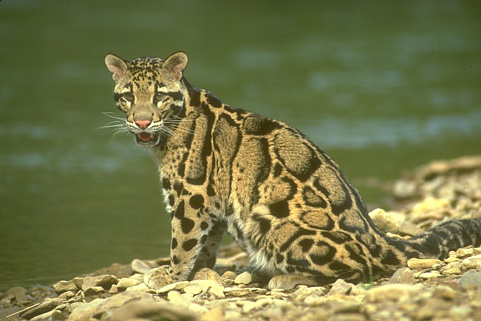
\includegraphics[width=\dimexpr\linewidth-20pt\relax]{160067} 
    \end{subfigure}  \\ \vspace{-5pt}    
    
    
    \begin{subfigure}[b]{\dimexpr0.23\textwidth+20pt\relax}
    	\centering
    	\makebox[20pt]{\raisebox{30pt}{ \rotatebox[origin=c]{90} {\small \textsf{\textbf{LAB}}} }}%
    	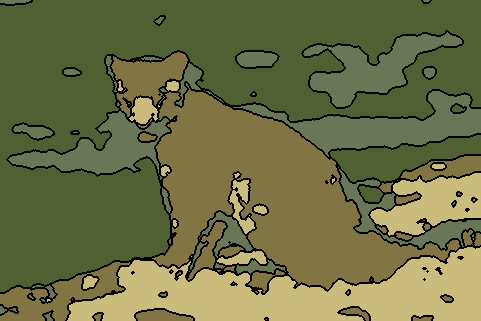
\includegraphics[width=\dimexpr\linewidth-20pt\relax]{160067_KMeans_const_segm_HSV} 
    \end{subfigure}      
%    ~ %add desired spacing between images, e. g. ~, \quad, \qquad, \hfill etc. 
      %(or a blank line to force the subfigure onto a new line)
    \begin{subfigure}[b]{0.23\textwidth}
    	\centering
        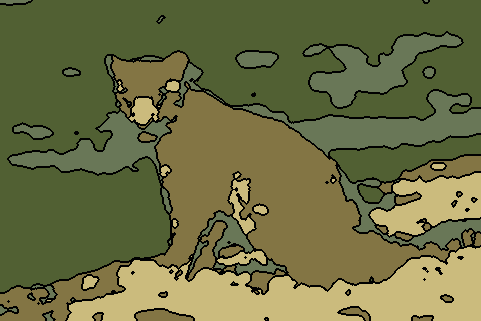
\includegraphics[height=67.68857pt]{160067_MiniBatchKMeans_const_segm_HSV}
    \end{subfigure}
%    ~ %add desired spacing between images, e. g. ~, \quad, \qquad, \hfill etc. 
      %(or a blank line to force the subfigure onto a new line)
    \begin{subfigure}[b]{0.23\textwidth}
    	\centering
        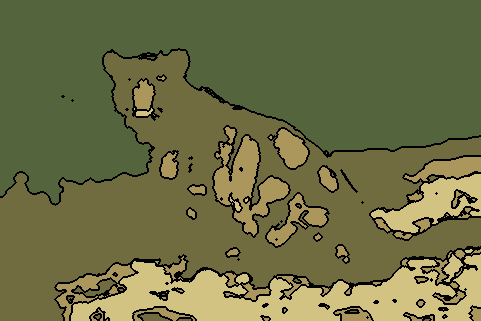
\includegraphics[height=67.68857pt]{160067_Birch_const_segm_LAB}
    \end{subfigure}
%    ~ %add desired spacing between images, e. g. ~, \quad, \qquad, \hfill etc. 
      %(or a blank line to force the subfigure onto a new line)
    \begin{subfigure}[b]{0.23\textwidth}
    	\centering
        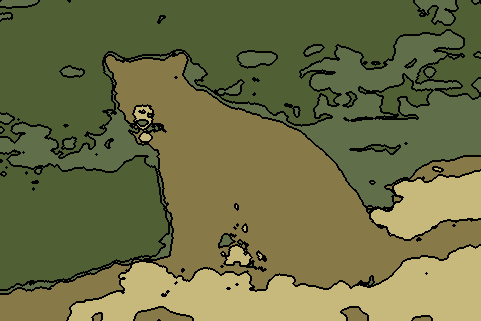
\includegraphics[height=67.68857pt]{160067_GaussianMixture_const_segm_HSV}
    \end{subfigure} \\ \vspace{-5pt}  
    
          
    \begin{subfigure}[b]{\dimexpr0.23\textwidth+20pt\relax}
    	\centering
    	\makebox[20pt]{\raisebox{30pt}{ \rotatebox[origin=c]{90} {\small \textsf{\textbf{HSV}}} }}%
    	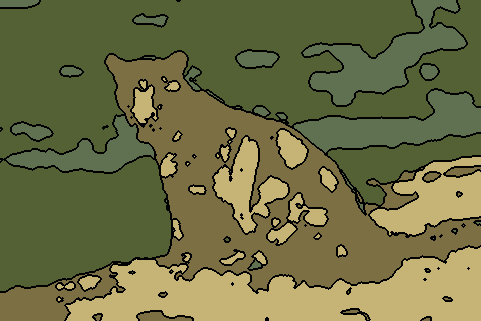
\includegraphics[width=\dimexpr\linewidth-20pt\relax]{160067_KMeans_const_segm_LAB} 
    \end{subfigure}      
%    ~ %add desired spacing between images, e. g. ~, \quad, \qquad, \hfill etc. 
      %(or a blank line to force the subfigure onto a new line)
    \begin{subfigure}[b]{0.23\textwidth}
    	\centering
        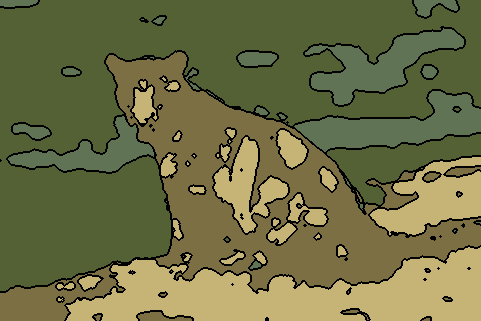
\includegraphics[height=67.68857pt]{160067_MiniBatchKMeans_const_segm_LAB}
    \end{subfigure}
%    ~ %add desired spacing between images, e. g. ~, \quad, \qquad, \hfill etc. 
      %(or a blank line to force the subfigure onto a new line)
    \begin{subfigure}[b]{0.23\textwidth}
    	\centering
        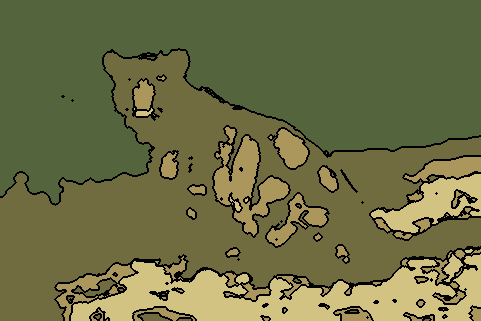
\includegraphics[height=67.68857pt]{160067_Birch_const_segm_LAB}
    \end{subfigure}
%    ~ %add desired spacing between images, e. g. ~, \quad, \qquad, \hfill etc. 
      %(or a blank line to force the subfigure onto a new line)
    \begin{subfigure}[b]{0.23\textwidth}
    	\centering
        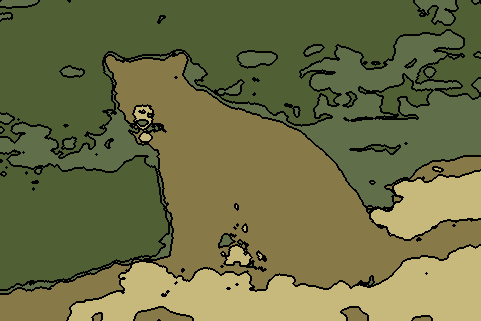
\includegraphics[height=67.68857pt]{160067_GaussianMixture_const_segm_HSV}
    \end{subfigure} \\ \vspace{-5pt}
    
           
    \begin{subfigure}[b]{\dimexpr0.23\textwidth+20pt\relax}
    	\centering
    	\makebox[20pt]{\raisebox{30pt}{ \rotatebox[origin=c]{90} {\small \textsf{\textbf{HSL}}} }}%
    	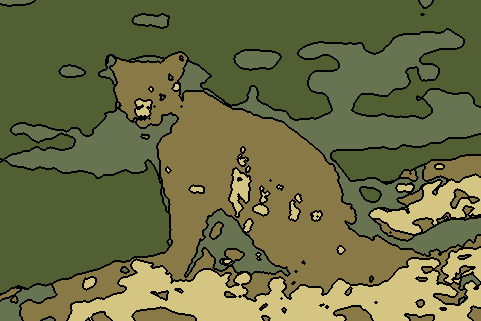
\includegraphics[width=\dimexpr\linewidth-20pt\relax]{160067_KMeans_const_segm_HSL} 
    	\caption{k-means}
    \end{subfigure}      
%    ~ %add desired spacing between images, e. g. ~, \quad, \qquad, \hfill etc. 
      %(or a blank line to force the subfigure onto a new line)
    \begin{subfigure}[b]{0.23\textwidth}
    	\centering
        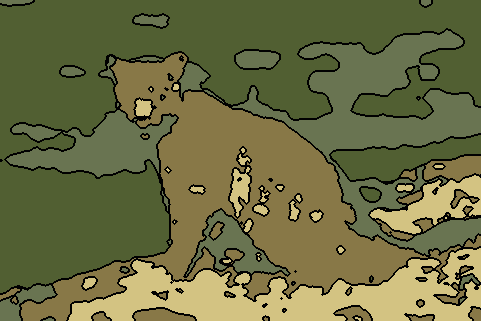
\includegraphics[height=67.68857pt]{160067_MiniBatchKMeans_const_segm_HSL}
        \caption{Fast k-means}
    \end{subfigure}
%    ~ %add desired spacing between images, e. g. ~, \quad, \qquad, \hfill etc. 
      %(or a blank line to force the subfigure onto a new line)
    \begin{subfigure}[b]{0.23\textwidth}
    	\centering
        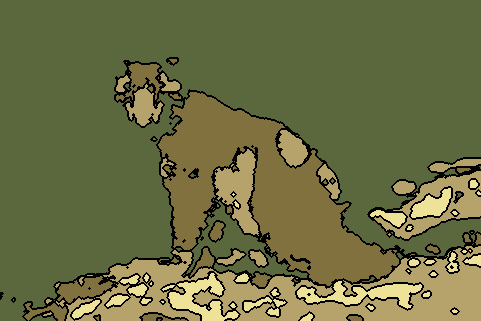
\includegraphics[height=67.68857pt]{160067_Birch_const_segm_HSL}
        \caption{Birch}
    \end{subfigure}
%    ~ %add desired spacing between images, e. g. ~, \quad, \qquad, \hfill etc. 
      %(or a blank line to force the subfigure onto a new line)
    \begin{subfigure}[b]{0.23\textwidth}
    	\centering
        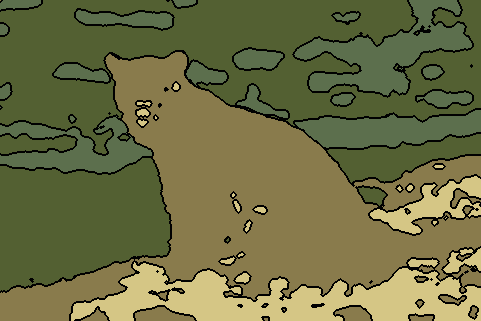
\includegraphics[height=67.68857pt]{160067_GaussianMixture_const_segm_HSL}
        \caption{Gaussian mixture}
    \end{subfigure} 
    
	\caption{Importance of the color space and the clustering algorithm in the image segmentation task using the feature space based on Gabor filters. BSDS lynx image segmentation results.}\label{fig:lynx_clustering_method_v_colorspace}    
\end{figure}


\begin{figure}[!ht]
         
    \begin{subfigure}[b]{\dimexpr0.23\textwidth+20pt\relax}
    	\centering
    	\makebox[20pt]{\raisebox{30pt}{ \rotatebox[origin=c]{90} {\small \textsf{\textbf{Input image}}} }}%
    	\includegraphics[width=\dimexpr\linewidth-20pt\relax]{43074} 
    \end{subfigure}  \\ \vspace{-5pt}   
    
    
    \begin{subfigure}[b]{\dimexpr0.23\textwidth+20pt\relax}
    	\centering
    	\makebox[20pt]{\raisebox{30pt}{ \rotatebox[origin=c]{90} {\small \textsf{\textbf{LAB}}} }}%
    	\includegraphics[width=\dimexpr\linewidth-20pt\relax]{43074_KMeans_const_segm_HSV} 
    \end{subfigure}      
%    ~ %add desired spacing between images, e. g. ~, \quad, \qquad, \hfill etc. 
      %(or a blank line to force the subfigure onto a new line)
    \begin{subfigure}[b]{0.23\textwidth}
    	\centering
        \includegraphics[height=67.68857pt]{43074_MiniBatchKMeans_const_segm_HSV}
    \end{subfigure}
%    ~ %add desired spacing between images, e. g. ~, \quad, \qquad, \hfill etc. 
      %(or a blank line to force the subfigure onto a new line)
    \begin{subfigure}[b]{0.23\textwidth}
    	\centering
        \includegraphics[height=67.68857pt]{43074_Birch_const_segm_LAB}
    \end{subfigure}
%    ~ %add desired spacing between images, e. g. ~, \quad, \qquad, \hfill etc. 
      %(or a blank line to force the subfigure onto a new line)
    \begin{subfigure}[b]{0.23\textwidth}
    	\centering
        \includegraphics[height=67.68857pt]{43074_GaussianMixture_const_segm_HSV}
    \end{subfigure} \\ \vspace{-5pt}
    
    
    \begin{subfigure}[b]{\dimexpr0.23\textwidth+20pt\relax}
    	\centering
    	\makebox[20pt]{\raisebox{30pt}{ \rotatebox[origin=c]{90} {\small \textsf{\textbf{HSV}}} }}%
    	\includegraphics[width=\dimexpr\linewidth-20pt\relax]{43074_KMeans_const_segm_LAB} 
    \end{subfigure}      
%    ~ %add desired spacing between images, e. g. ~, \quad, \qquad, \hfill etc. 
      %(or a blank line to force the subfigure onto a new line)
    \begin{subfigure}[b]{0.23\textwidth}
    	\centering
        \includegraphics[height=67.68857pt]{43074_MiniBatchKMeans_const_segm_LAB}
    \end{subfigure}
%    ~ %add desired spacing between images, e. g. ~, \quad, \qquad, \hfill etc. 
      %(or a blank line to force the subfigure onto a new line)
    \begin{subfigure}[b]{0.23\textwidth}
    	\centering
        \includegraphics[height=67.68857pt]{43074_Birch_const_segm_LAB}
    \end{subfigure}
%    ~ %add desired spacing between images, e. g. ~, \quad, \qquad, \hfill etc. 
      %(or a blank line to force the subfigure onto a new line)
    \begin{subfigure}[b]{0.23\textwidth}
    	\centering
        \includegraphics[height=67.68857pt]{43074_GaussianMixture_const_segm_HSV}
    \end{subfigure} \\ \vspace{-5pt}
    
    
    \begin{subfigure}[b]{\dimexpr0.23\textwidth+20pt\relax}
    	\centering
    	\makebox[20pt]{\raisebox{30pt}{ \rotatebox[origin=c]{90} {\small \textsf{\textbf{HSL}}} }}%
    	\includegraphics[width=\dimexpr\linewidth-20pt\relax]{43074_KMeans_const_segm_HSL} 
    	\caption{k-means}
    \end{subfigure}      
%    ~ %add desired spacing between images, e. g. ~, \quad, \qquad, \hfill etc. 
      %(or a blank line to force the subfigure onto a new line)
    \begin{subfigure}[b]{0.23\textwidth}
    	\centering
        \includegraphics[height=67.68857pt]{43074_MiniBatchKMeans_const_segm_HSL}
        \caption{Fast k-means}
    \end{subfigure}
%    ~ %add desired spacing between images, e. g. ~, \quad, \qquad, \hfill etc. 
      %(or a blank line to force the subfigure onto a new line)
    \begin{subfigure}[b]{0.23\textwidth}
    	\centering
        \includegraphics[height=67.68857pt]{43074_Birch_const_segm_HSL}
        \caption{Birch}
    \end{subfigure}
%    ~ %add desired spacing between images, e. g. ~, \quad, \qquad, \hfill etc. 
      %(or a blank line to force the subfigure onto a new line)
    \begin{subfigure}[b]{0.23\textwidth}
    	\centering
        \includegraphics[height=67.68857pt]{43074_GaussianMixture_const_segm_HSL}
        \caption{Gaussian mixture}
    \end{subfigure} 
    
	\caption{Importance of the color space and the clustering algorithm in the image segmentation task using the feature space based on Gabor filters. BSDS pheasant image segmentation results.}\label{fig:pheasant_clustering_method_v_colorspace}    
\end{figure}



\paragraph{Number of clusters in the data.} 
Determining the number of segments to detect when using clustering algorithms as an image segmentation technique is a frequent problem. The four algorithms we present here for image segmentation need the $k$ parameter to specify the number of clusters to find. Although there are techniques to estimate the number of regions in the image, these strategies involve one more stage of processing, which is reflected in the final segmentation calculation time. To find the optimal number of regions, we use the GT of the BSDS500. Since each image in the database contains between 5 and 11 human-made segmentations $\mathcal{S}=\{\mathcal{S}_1, \mathcal{S}_1, \cdots, \mathcal{S}_n\}$, we take $k$ as the maximum and the minimum number of segments found by the human observers for each image. 
\begin{eqnarray}
	k = \mathrm{max}(\mathcal{S}) \\
	k = \mathrm{min}(\mathcal{S})
\end{eqnarray}

Figure \ref{fig:Gmixture_starfish_segms_diff_k} shows the segmentation result of a BSDS image by manually setting $k$ with fixed values of 3 and 4 segments and defining $k$ as the number of maximum and minimum segments of the GT. In this particular case of the starfish image, the maximum number of annotated segments by a human observer is 92, while the minimum number of annotated segments is 6. The clustering algorithm used for this experiment is the Gaussian mixture in using the feature space from the LAB color space.


\begin{figure}[!ht]
    
    \begin{subfigure}[b]{0.23\textwidth}
        \includegraphics[width=\textwidth]{12003}
        \caption{Input image}
    \end{subfigure} \\  \vspace{5pt}
    
    \begin{subfigure}[b]{0.23\textwidth}
    	\centering
    	\includegraphics[width=\textwidth]{12003_GaussianMixture_3_segm}
        \caption{$k=3$ }
    \end{subfigure} ~
    \begin{subfigure}[b]{0.23\textwidth}
    	\centering
        \includegraphics[width=\textwidth]{12003_GaussianMixture_4_segm}
        \caption{$k=4$}
    \end{subfigure} ~
    \begin{subfigure}[b]{0.23\textwidth}
    	\centering
    	\includegraphics[width=\textwidth]{12003_GaussianMixture_min_segm}
        \caption{$k=\mathrm{min}(\mathcal{S})$}
    \end{subfigure} ~¨
    \begin{subfigure}[b]{0.23\textwidth}
    	\centering
    	\includegraphics[width=\textwidth]{12003_GaussianMixture_max_segm}
        \caption{$k=\mathrm{max}(\mathcal{S})$}
    \end{subfigure} 
        	    
    \caption{Effect of the choice of the number of clusters $k$ in clustering algorithms as segmentation methods.}\label{fig:Gmixture_starfish_segms_diff_k}    
\end{figure}

The image segmentation results show various phenomena. The first one is the big difference between human-made segmentations; the annotation with 92 regions implies a very detailed segmentation, while the annotation with 6 regions does not reflect the most basic segmentation of the image: two objects, the starfish and the background. Both of these extrema, despite their substantial difference, are considered as ground truth.

This behavior is of vital importance in the evaluation of a segmentation algorithm since the scores are a function of the GT. In the case of the BSDS500, increasing $k$ means finding more regions that coincide with the GT regions, so the recall score increases; however, the precision of the regions found is very low. On the other hand, by decreasing, $k$ we detect fewer regions, which favors the precision score but affects the recall. Figure \ref{fig:PR_boxplot_scores_min_max_clusters} shows this phenomenon with the boxplots of the precision and recall scores of the different clustering methods using $k = \mathrm{min}(\mathcal{S})$ and $k = \mathrm{max}(\mathcal{S})$. Therefore, the optimal number of clusters $k$ should keep a balance between maximum data compression using a single cluster and maximum precision when assigning each pixel to its own cluster.


\begin{figure}[!ht]
    \centering
    \begin{subfigure}[b]{0.49\textwidth}
        \includegraphics[width=\textwidth]{PrecisionRecall_boxplot_min_nclusters_LAB}
        \caption{$k=\mathrm{min}(\mathcal{S})$}
    \end{subfigure}   
    \begin{subfigure}[b]{0.49\textwidth}
    	\centering
    	\includegraphics[width=\textwidth]{PrecisionRecall_boxplot_max_nclusters_LAB}
        \caption{$k=\mathrm{max}(\mathcal{S})$}
    \end{subfigure}     
%    \begin{subfigure}[b]{0.3\textwidth}
%    	\centering
%    	\includegraphics[width=\textwidth]{PrecisionRecall_boxplot_const_nclusters_LAB}
%        \caption{$k=4$}
%    \end{subfigure}
    
        	    
    \caption{Synthetic image k-means segmentation results.}\label{fig:PR_boxplot_scores_min_max_clusters}    
\end{figure}

%\paragraph{Clustering computation time } % pending !!!

\subsubsection{Results}
The two previous experiments show that the segmentation of real images is a complex task in which the result depends on various parameters such as the configuration of the input space, the number of segments, etc. Here we show some segmentation results (see figure \ref{fig:BSD_clustering_results}) using the feature space derived from the HSV-based luminance-chrominance color space and the four segmentation algorithms presented in this section.

The segmentation results are obtained by setting $k = 4$ for all images. Figure \ref{fig:PR_boxplot_scores} shows the precision and recall boxplots of each of the segmentation algorithms using the three different color spaces (HSV, HSL, and LAB).

\begin{figure}[!ht]
    \centering
    \begin{subfigure}[b]{0.49\textwidth}
        \includegraphics[width=\textwidth]{PrecisionRecall_boxplot_const_nclusters_HSL}
        \caption{HSL}
    \end{subfigure}
    \begin{subfigure}[b]{0.49\textwidth}
    	\centering
    	\includegraphics[width=\textwidth]{PrecisionRecall_boxplot_const_nclusters_HSV}
        \caption{HSV}
    \end{subfigure}\\     
    \begin{subfigure}[b]{0.49\textwidth}
    	\centering
        \includegraphics[width=\textwidth]{PrecisionRecall_boxplot_const_nclusters_LAB}
        \caption{LAB}
    \end{subfigure} 
        	    
    \caption{Boxplots of precision and recall scores of the different clustering methods and the different color spaces. For the three plots, the number of clusters was set constant at $k=4$.}\label{fig:PR_boxplot_scores}    
\end{figure}



\begin{figure}[!ht]
         
    \begin{subfigure}[t]{\dimexpr0.23\textwidth+20pt\relax}
    	\centering
    	\makebox[20pt]{\raisebox{30pt}{ \rotatebox[origin=c]{90} {\small \textsf{\textbf{Input image}}} }}%
    	\includegraphics[width=\dimexpr\linewidth-20pt\relax]{100007} 
    \end{subfigure}      
%    ~ %add desired spacing between images, e. g. ~, \quad, \qquad, \hfill etc. 
      %(or a blank line to force the subfigure onto a new line)
    \begin{subfigure}[b]{0.23\textwidth}
    	\centering
        \includegraphics[height=67.68857pt]{101084}
    \end{subfigure}
%    ~ %add desired spacing between images, e. g. ~, \quad, \qquad, \hfill etc. 
      %(or a blank line to force the subfigure onto a new line)
    \begin{subfigure}[b]{0.23\textwidth}
    	\centering
        \includegraphics[height=67.68857pt]{175083}
    \end{subfigure}
%    ~ %add desired spacing between images, e. g. ~, \quad, \qquad, \hfill etc. 
      %(or a blank line to force the subfigure onto a new line)
    \begin{subfigure}[b]{0.23\textwidth}
    	\centering
        \includegraphics[height=67.68857pt]{181021}
    \end{subfigure} \\ 
    
    \begin{subfigure}[t]{\dimexpr0.23\textwidth+20pt\relax}
    	\centering
    	\makebox[20pt]{\raisebox{30pt}{ \rotatebox[origin=c]{90} {\small \textsf{\textbf{Kmeans}}} }}%
    	\includegraphics[width=\dimexpr\linewidth-20pt\relax]{100007_Kmeans_const_segm} 
    \end{subfigure}      
%    ~ %add desired spacing between images, e. g. ~, \quad, \qquad, \hfill etc. 
      %(or a blank line to force the subfigure onto a new line)
    \begin{subfigure}[b]{0.23\textwidth}
    	\centering
        \includegraphics[height=67.68857pt]{101084_Kmeans_const_segm}
    \end{subfigure}
%    ~ %add desired spacing between images, e. g. ~, \quad, \qquad, \hfill etc. 
      %(or a blank line to force the subfigure onto a new line)
    \begin{subfigure}[b]{0.23\textwidth}
    	\centering
        \includegraphics[height=67.68857pt]{175083_Kmeans_const_segm}
    \end{subfigure}
%    ~ %add desired spacing between images, e. g. ~, \quad, \qquad, \hfill etc. 
      %(or a blank line to force the subfigure onto a new line)
    \begin{subfigure}[b]{0.23\textwidth}
    	\centering
        \includegraphics[height=67.68857pt]{181021_Kmeans_const_segm}
    \end{subfigure} \\ 
       
    \begin{subfigure}[t]{\dimexpr0.23\textwidth+20pt\relax}
    	\centering
    	\makebox[20pt]{\raisebox{30pt}{ \rotatebox[origin=c]{90} {\small \textsf{\textbf{Fast Kmeans}}} }}%
    	\includegraphics[width=\dimexpr\linewidth-20pt\relax]{100007_MiniBatchKMeans_const_segm} 
    \end{subfigure}      
%    ~ %add desired spacing between images, e. g. ~, \quad, \qquad, \hfill etc. 
      %(or a blank line to force the subfigure onto a new line)
    \begin{subfigure}[b]{0.23\textwidth}
    	\centering
        \includegraphics[height=67.68857pt]{101084_MiniBatchKMeans_const_segm}
    \end{subfigure}
%    ~ %add desired spacing between images, e. g. ~, \quad, \qquad, \hfill etc. 
      %(or a blank line to force the subfigure onto a new line)
    \begin{subfigure}[b]{0.23\textwidth}
    	\centering
        \includegraphics[height=67.68857pt]{175083_MiniBatchKMeans_const_segm}
    \end{subfigure}
%    ~ %add desired spacing between images, e. g. ~, \quad, \qquad, \hfill etc. 
      %(or a blank line to force the subfigure onto a new line)
    \begin{subfigure}[b]{0.23\textwidth}
    	\centering
        \includegraphics[height=67.68857pt]{181021_MiniBatchKMeans_const_segm}
    \end{subfigure} \\ 
    
    \begin{subfigure}[t]{\dimexpr0.23\textwidth+20pt\relax}
    	\centering
    	\makebox[20pt]{\raisebox{30pt}{ \rotatebox[origin=c]{90} {\small \textsf{\textbf{Guassian mixture}}} }}%
    	\includegraphics[width=\dimexpr\linewidth-20pt\relax]{100007_GaussianMixture_const_segm} 
    \end{subfigure}      
%    ~ %add desired spacing between images, e. g. ~, \quad, \qquad, \hfill etc. 
      %(or a blank line to force the subfigure onto a new line)
    \begin{subfigure}[b]{0.23\textwidth}
    	\centering
        \includegraphics[height=67.68857pt]{101084_GaussianMixture_const_segm}
    \end{subfigure}
%    ~ %add desired spacing between images, e. g. ~, \quad, \qquad, \hfill etc. 
      %(or a blank line to force the subfigure onto a new line)
    \begin{subfigure}[b]{0.23\textwidth}
    	\centering
        \includegraphics[height=67.68857pt]{175083_GaussianMixture_const_segm}
    \end{subfigure}
%    ~ %add desired spacing between images, e. g. ~, \quad, \qquad, \hfill etc. 
      %(or a blank line to force the subfigure onto a new line)
    \begin{subfigure}[b]{0.23\textwidth}
    	\centering
        \includegraphics[height=67.68857pt]{181021_GaussianMixture_const_segm}
    \end{subfigure} \\ 
    
    \begin{subfigure}[t]{\dimexpr0.23\textwidth+20pt\relax}
    	\centering
    	\makebox[20pt]{\raisebox{30pt}{ \rotatebox[origin=c]{90} {\small \textsf{\textbf{Birch}}} }}%
    	\includegraphics[width=\dimexpr\linewidth-20pt\relax]{100007_Birch_const_segm} 
    \end{subfigure}      
%    ~ %add desired spacing between images, e. g. ~, \quad, \qquad, \hfill etc. 
      %(or a blank line to force the subfigure onto a new line)
    \begin{subfigure}[b]{0.23\textwidth}
    	\centering
        \includegraphics[height=67.68857pt]{101084_Birch_const_segm}
    \end{subfigure}
%    ~ %add desired spacing between images, e. g. ~, \quad, \qquad, \hfill etc. 
      %(or a blank line to force the subfigure onto a new line)
    \begin{subfigure}[b]{0.23\textwidth}
    	\centering
        \includegraphics[height=67.68857pt]{175083_Birch_const_segm}
    \end{subfigure}
%    ~ %add desired spacing between images, e. g. ~, \quad, \qquad, \hfill etc. 
      %(or a blank line to force the subfigure onto a new line)
    \begin{subfigure}[b]{0.23\textwidth}
    	\centering
        \includegraphics[height=67.68857pt]{181021_Birch_const_segm}
    \end{subfigure}     
	\caption{Segmentation results using different segmentation algorithms and HSV color space. The number of segments to find is fixed at $ k = 4 $ for all images. }\label{fig:BSD_clustering_results}    
\end{figure}


\subsection{High-level Texture Features}\label{sec:high_level_features}
This section addresses the methodology for the extraction of high-level local texture features. To this end, we base the study of image textures on the Gabor filters. We obtain a spectral decomposition of the image through the convolution of the image with the filter bank. The spectral image decomposition allows us to obtain the following high-level features:

\begin{itemize}
	\item Fundamental Frequency
	\item Dominant Orientation
	\item Maximal Response
	\item Orientation Entropy
	\item Orientability
	\item Texturability 
	\item Perceptual Window, Mean Color, and Principal Colors
\end{itemize}

\subsubsection{Fundamental Frequency}
As we mentioned earlier, a texture is generated by contrast variations at a particular frequency or with a specific, repeating pattern. Although a texture may contain variations at multiple frequencies, there is only one that stands out and is more perceptive to the human eye. We call this \textit{fundamental frequency}.

The fundamental frequency is a concept commonly used in music, acoustics, signal theory, and speech analysis \citep{Benward:BOOK:2014}, \citep{Sigmund:ITC:2013}. This is defined as the lowest frequency of a harmonic series representing periodic parts of a speech signal. To our knowledge, this concept has not been applied under the exact definition for image processing and texture analysis. The closest approach is that of \cite{Kamarainen.Kyrki.ea:ICPR:2002}, who defines it as the frequency within the Gabor filter bank frequencies that gives the maximum response for each filter bank orientation. They use the fundamental frequency as a feature to characterize and recognize objects \citep{Kamarainen.Kyrki.ea:DSP:2002}; however, it is prone to failure when there are multiple objects of the same size in the image or when the objects' shapes are not precise.

We propose to obtain the fundamental frequency of textures from the image spectral decomposition $\widetilde{e}_{c, f, \theta}$ Eq. \eqref{eq:gabor_energy_smth}, following the definition by signal theory. The first step is to obtain the filter responses for each frequency, taking into account all the filter bank orientations. We do this procedure for each channel of the image $c=\{L, \RE(C), \IM(C)\}$.

\begin{equation}
	\widetilde{e}_{c, f} =  \underset{\theta }{\sum} \widetilde{e}_{c, f, \theta}  \label{eq:gabor_energy_ch_freq}
\end{equation}

From the response vector Eq. \eqref{eq:gabor_energy_ch_freq}, we can calculate the fundamental frequency $\widehat{f_c}$ of each channel of the image as
\begin{equation}
	\widetilde{f_c} =  \underset{f}{\arg} (\widetilde{e}_{c, f}) ~|~ \widetilde{e}_{c, f} > \frac{\max(\widetilde{e}_{c, f})}{2} \label{eq:fundamental_frequencygabor_ch}
\end{equation}
where $\max(\widetilde{e}_{c, f})/2$ is a threshold value that filters out the small responses generated low-level frequencies or zones without texture. The corresponding frequency to such zones is set to the zero frequency ($f_0$), given by the image's DC component.

Finally, the fundamental frequency for the complete image (for all three channels) is obtained as
\begin{equation}
	\widetilde{f}(x,y) =  \max(\widetilde{f_c}(x,y))  \label{eq:fundamental_freq}
\end{equation}

We show the fundamental frequency of the different areas of the synthetic image in figure \ref{fig:fund_freq_synth}. In the figure, we can see how our approach recovers each zone's lowest frequency within the filter center frequencies. This effect is most visible in image zone 7 (between pixels 1200 and 1400), which contains a texture that varies at two different frequencies, $f = 1/8$ and $f = 1/32$ (see table \ref{tab:synthetic_image_components} and Fig. \ref{fig:synthetic_color_texture_image}). The lowest frequency in this zone is $f = 1/32$, which corresponds to the found fundamental frequency. On the other hand, the fundamental frequency for zone 1 (the yellow textureless zone between pixels 0 and 200) corresponds to the frequency zero $f_0$, which we obtain by filtering the image with a low-level filter such as a Gaussian filter larger than the lowest frequency filter in Gabor's filter bank.

\begin{figure}[!ht]
	\includegraphics[width=\textwidth]{fund_freq_synth}
    \caption{Fundamental frequency in the synthetic test image.}
    \label{fig:fund_freq_synth}
\end{figure}

\subsubsection{Dominant Orientation}
Similarly, as in the frequency dimension, a texture can be generated at different orientations; however, there is an orientation in which spatial variations stand out more to the human eye. We call this orientation the \textit{dominant orientation}.

To obtain the dominant orientation of a texture, we need first to obtain the Gabor responses along the three image channels.
\begin{equation}
	\widetilde{e}_{f, \theta} = \underset{c}{\sum} \widetilde{e}_{c, f, \theta}  \label{eq:gabor_energy_freq_orient}
\end{equation}

Then, we define the dominant orientation as 
\begin{equation}
	\widetilde{\theta}(x,y) =  \arg\max (\widetilde{e}_{f, \theta}) ~|~ f = \widetilde{f} \label{eq:dominant_orient}
\end{equation}

The dominant orientation denotes the angle within the Gabor filter bank's orientations at the fundamental frequency that allows recovering the higher Gabor response from the image after convolution.

We show the dominant orientations of our synthetic test image in figure \ref{fig:dom_orient_synth}. We see the relationship between the dominant orientation and the fundamental frequency in the values retrieved for the first zone of the synthetic image (between pixels 0 and 200). Since it does not contain any texture, its fundamental frequency is the frequency zero; therefore, the dominant orientation is random. The rest of the zones (from pixel 200 to 1400) contains textures created by vertical lines, i.e., at an angle of $0^\circ$; however, in the last zone, which contains two textures, we recover $90^\circ$ as dominant orientation since the fundamental frequency is that of the texture created with horizontal lines. 

\begin{figure}[!ht]
	\includegraphics[width=\textwidth]{dom_orient_synth}
    \caption{Dominant orientation in the synthetic test image.}
    \label{fig:dom_orient_synth}
\end{figure}

\subsubsection{Maximal Response}
The \textit{maximal response} is a feature that reflects the contribution of the various components of the color information (luminance and chrominance) and the texture (frequency and orientation). To correctly capture such information, we first retrieve the maximum Gabor response along with the frequency and orientation axis for each color channel, and later we add the maximum contributions of each channel of the complex color space. The expression that denotes the maximum response of the filter is
\begin{equation}
	\widetilde{e}_{max}(x,y) = \underset{c}{\sum} \underset{f, \theta}{\max} (\widetilde{e}_{c, f, \theta}) \label{eq:max_energy}
\end{equation}

We can see the maximal response of the synthetic image in figure \ref{fig:max_energy_synth}. This feature highlights sudden dynamic changes (significant Gabor responses) and shadows textureless zones in the image. Note that the maximal response of the last zone of the synthetic image (zone with two textures) is less than the other textured areas; this is because this texture's energy is distributed between Gabor's responses with $f=1/8, \theta=0^\circ$ and $f=1/32, \theta=90^\circ$.

\begin{figure}[!ht]
	\includegraphics[width=\textwidth]{max_energy_synth}
    \caption{Maximum filter response of the synthetic test image.}
    \label{fig:max_energy_synth}
\end{figure}

\subsubsection{Orientation Entropy}
Initially, the concept of entropy is a measure from Physics adapted to the information theory to calculate the amount of information stored in a particular signal. We adapt this measure to calculates the randomness of the texture's orientation in the Gabor responses distribution.  We call this feature \textit{orientation entropy}.

We obtain the orientation entropy $h$ by multiplying a probability vector by its logarithm. Since we use the image in a complex color space, we first obtain the entropy for each image channel.
\begin{gather}
    \widetilde{h_c}(x,y) = -\sum_{\theta} \overline{e}_{c, \theta} \log (\overline{e}_{c, \theta}) \label{eq:entropy_orient_ch}
\end{gather}

We obtain the probability $\widetilde{h_c}(x,y)$ by adding the Gabor responses along the frequency axis and dividing it by the total Gabor response along the three image channels.
\begin{equation}
	\overline{e}_{c, \theta} =  \frac{\sum_f \widetilde{e}_{c, f, \theta}}{\sum_{c, f, \theta}\widetilde{e}_{c, f, \theta} }  \label{eq:gabor_energy_ch_orient_prob}
\end{equation}

Each value of the vector indicates the probability that the Gabor filter response corresponds to a given orientation. If the vector values are of similar magnitude, the vector has no defined orientation; that is, the value response is likely to come from any filter. On the other hand, if the probability vector values are unequal, the response is very likely to belong to a well-defined orientation zone.

The orientation entropy can be normalized since we know the number of orientation angles $N$ in the filter bank, meaning that the maximum entropy values is given by 
\begin{equation}
    h_{max} = -\log\left(\frac{1}{N}\right) \label{eq:max_entropy_orient} 
\end{equation}

The min value between the three image channels' normalized entropies gives the image's total orientation entropy.
\begin{gather}
    \widetilde{h}(x,y) = \min(\widetilde{h_c}) \label{eq:entropy_orient}
\end{gather}

This feature is helpful to identify the isotropic zones on the image. A high entropy value of entropy indicates a zone with random orientation, whereas a low entropy value indicates a zone with a well-defined orientation (anisotropic texture). We depict the orientation entropy of the synthetic image in figure \ref{fig:entropy_orient_synth}.

\begin{figure}[!ht]
	\includegraphics[width=\textwidth]{entropy_orient_synth}
    \caption{Orientation entropy of the synthetic test image.}
    \label{fig:entropy_orient_synth}
\end{figure}

%\begin{figure}[!ht]
%    \centering
%    \begin{subfigure}[b]{\textwidth}    	
%    	\includegraphics[width=\textwidth]{fund_freq_synth}
%        \caption{Fundamental frequency}
%        \label{fig:fund_freq_synth}
%    \end{subfigure}\\
%    \begin{subfigure}[b]{\textwidth}
%    	\includegraphics[width=\textwidth]{dom_orient_synth}
%        \caption{Dominant orientation}
%        \label{fig:dom_orient_synth}
%    \end{subfigure}\\
%    \begin{subfigure}[b]{\textwidth}
%    	\includegraphics[width=\textwidth]{max_energy_synth}
%        \caption{Maximum filter response}
%        \label{fig:max_energy_synth}
%    \end{subfigure}\\
%    \begin{subfigure}[b]{\textwidth}
%    	\includegraphics[width=\textwidth]{entropy_orient_synth}
%        \caption{Entropy}
%        \label{fig:entropy_orient_synth}
%    \end{subfigure}\\
%    \begin{subfigure}[b]{\textwidth}
%    	\includegraphics[width=\textwidth]{orientability_synth}
%        \caption{Orientability}
%        \label{fig:orientability_synth}
%    \end{subfigure}\\
%    \begin{subfigure}[b]{\textwidth}
%    	\includegraphics[width=\textwidth]{texturality_synth}
%        \caption{Texturality}
%        \label{fig:texturality_synth}
%    \end{subfigure}    
%                  
%    \caption{High-level texture feautures computed form the synthetic image test.}\label{fig:high_level_features_synth}    
%\end{figure}

\subsubsection{Orientability}
This feature is a visual property for understanding and interpreting the texture information of an image. The \textit{orientability} is a composite feature that allows us to enhance those texture zones with a well-defined orientation angle and hide the isotropic ones.

We obtain the orientability by weighing the dominant orientation Eq. \eqref{eq:dominant_orient} by the orientation entropy Eq. \eqref{eq:entropy_orient}. We depict this feature in a three-channel image. The first channel is the luminance dimension of the input image $L(x,y)$. This channel serves as a canvas to put the color given the dominant orientation $\widetilde{\theta}$, which can be represented into a cyclic colormap such as the HSV. The last channel is an alpha channel given by the opposite of the orientation entropy $\widetilde{h}$. This last channel is a transparency channel that acts as a weight for the dominant orientation. That is,

\begin{gather}
    \text{channel 1} = L(x,y) \\
    \text{channel 2} = \widetilde{\theta}(x,y) \\
    \text{alpha channel}= 1 - \widetilde{h}(x,y)
\end{gather}

We can see the orientability of the synthetic image in figure \ref{fig:orientability_synth}. This figure shows how the dominant orientation of the textureless zones (zone 1) and the zone with two textures (zone 7) are less saturated than the rest of the zones. 

\begin{figure}[!ht]
	\includegraphics[width=\textwidth]{orientability_synth}
    \caption{Orientability of the synthetic test image.}
    \label{fig:orientability_synth}
\end{figure}

\subsubsection{Texturability}
The \textit{texturality} is a visual feature that joins the fundamental frequency Eq. \eqref{eq:fundamental_freq} and the maximal Gabor response Eq. \eqref{eq:max_energy}. We represent this feature in a three-channel image. We map the fundamental frequency values $\widetilde{f}$ to a diverging color map and use it as channel 2 of the composed image. TThen, the alpha channel of the fundamental frequency is given by the Gabor filter's maximal response $\widetilde{e}_{max}$. Finally, we use the input image's luminance channel $L(x,y)$ as a canvas to show the composite feature. That is,

\begin{gather}
    \text{channel 1} = L(x,y) \\
    \text{channel 2} = \widetilde{f}(x,y) \\
    \text{alpha channel} = \widetilde{e}_{max}(x,y) \\
\end{gather}

Figure \ref{fig:texturality_synth} shows the texturality feature computed for the synthetic texture image. We can see how the fundamental frequency colors are shadowed by the maximal response, specifically at the textureless zone (zone 1) and the zone with two textures (zone 7).

\begin{figure}[!ht]
	\includegraphics[width=\textwidth]{texturality_synth}
    \caption{Texturality of the synthetic test image.}
    \label{fig:texturality_synth}
\end{figure}

%\begin{figure}[!ht]
%    \centering
%    \begin{subfigure}[b]{\textwidth}
%    	\includegraphics[width=\textwidth]{orientability_synth}
%        \caption{Orientability}
%        \label{fig:orientability_synth}
%    \end{subfigure}\\
%    \begin{subfigure}[b]{\textwidth}
%    	\includegraphics[width=\textwidth]{texturality_synth}
%        \caption{Texturality}
%        \label{fig:texturality_synth}
%    \end{subfigure}    
%                  
%    \caption{High-level texture feautures computed form the synthetic image test.}\label{fig:composite_high_level_features_synth}    
%\end{figure}

\subsubsection{Perceptual Window, Mean Color, and Principal Colors}
The Gabor function analysis in chapter \ref{ch:gabor_filter_description} for designing an optimized Gabor filter bank includes the computation of an adaptative Gaussian envelope (cf. Eq. \eqref{eq:1D_gabor_support}). The adaptative support is a function of the Gabor function's central frequency. We state that the filter support $\kappa$ of the fundamental frequency $\widetilde{f}$ contains the most representative information about the period of the texture of each pixel in the image. Since we know each pixel's fundamental frequency, we can recover their \textit{perceptual window}, which is the minimum window that describes a texture.

The perceptual window is given by the inverse of the fundamental frequency, such that
\begin{gather}
    \widetilde{T} = \frac{1}{\widetilde{f}} \label{eq:perceptual_window}
\end{gather}

The perceptual window allows us to compute some other features, including the mean color and the two principal texture color-former of each window. The computation is straightforward. We take the mean value of the color pixel values inside the perceptual window to obtain the mean color. For the texture-forming colors, we apply a PCA to compute the two principal components in the window.

Figure \ref{fig:colors_high_level_features_synth} shows the set of features resulting from the perceptual window. Subfigure \ref{fig:perceptual_mean_color_synth} shows the window of some pixels (chosen randomly); in this subfigure, we see how the perceptual window covers at least one period of the texture. In the two-textures zone, the perceptual window size corresponds to the period of the texture generated with horizontal contrast changes, while the yellow zone (without texture) has the largest window. 

We can see the mean colors of each textured region of the synthetic image in subfigure \ref{fig:perceptual_mean_color_synth}. We remember that we created the synthetic image using primary colors of the chromatic circle color representation. Therefore, we can find the mean colors of each region in the complex chromatic circle. For example, for zones 2 and 3, where we combine the colors of the imaginary and real axis of the complex chromatic circle (red and cyan for zone 2, and green and violet for zone 3), the mean color is the color at the center of the complex chromatic circle, that is, gray. For better comprehension, we invite the reader to analyze subfigure \ref{fig:perceptual_mean_color_synth} together with table \ref{tab:synthetic_image_components} and figure \ref{fig:color_complex_plane}.

Finally, looking at subfigures \ref{fig:perceptual_color1_synth} and \ref{fig:perceptual_color2_synth}, we can corroborate that we can recover the synthetic image's texture-forming colors from the multi-spectral image decomposition proposed in this document (see table \ref{tab:synthetic_image_components} for the reference of the texture-forming colors).

\begin{figure}[!ht]
    \centering
    \begin{subfigure}[b]{\textwidth}
    	\includegraphics[width=\textwidth]{perceptual_windows_synth_25}
        \caption{Examples of pecerptual windows}
        \label{fig:perceptual_windows_synth_25}
    \end{subfigure}\\
    \begin{subfigure}[b]{\textwidth}
    	\includegraphics[width=\textwidth]{perceptual_mean_color_synth}
        \caption{Perceptual window's mean color}
        \label{fig:perceptual_mean_color_synth}
    \end{subfigure}\\
    \begin{subfigure}[b]{\textwidth}
    	\includegraphics[width=\textwidth]{perceptual_color1_synth}
        \caption{Perceptual window's first texture-forming color}
        \label{fig:perceptual_color1_synth}
    \end{subfigure}\\
    \begin{subfigure}[b]{\textwidth}
    	\includegraphics[width=\textwidth]{perceptual_color2_synth}
        \caption{Perceptual window's second texture-forming color}
        \label{fig:perceptual_color2_synth}
    \end{subfigure}    
                  
    \caption{Synthetic image's high-level texture features derived from the fundamental frequency.}\label{fig:colors_high_level_features_synth}    
\end{figure}


In the figures \ref{fig:high_level_features_zebre} and \ref{fig:colors_high_level_features_zebre}, we show the different high-level texture features presented in this section calculated for a natural image of the BSDS. In that particular example, for the black-and-white striped zebras, the expected mean color is grey, and the two texture-forming colors are black and white. Note in figure \ref{fig:colors_high_level_features_zebre} how the two colors are not purely black and white when the stripes' period does not correspond exactly to the window.

\begin{figure}[!ht] 
	\centering
	\begin{subfigure}[b]{0.49\textwidth}
    	\includegraphics[width=\textwidth]{16068}
        \caption{Input image}
    \end{subfigure}
    \begin{subfigure}[b]{0.49\textwidth}
    	\includegraphics[width=\textwidth]{fund_freq_16068}
        \caption{Fundamental frequency}
        \label{fig:fund_freq_16068}
    \end{subfigure}
    \begin{subfigure}[b]{0.49\textwidth}
    	\includegraphics[width=\textwidth]{dom_orient_16068}
        \caption{Dominant orientation}
        \label{fig:dom_orient_16068}
    \end{subfigure}\\
    \begin{subfigure}[b]{0.49\textwidth}
    	\includegraphics[width=\textwidth]{max_energy_16068}
        \caption{Maximum filter response}
        \label{fig:max_energy_16068}
    \end{subfigure}
    \begin{subfigure}[b]{0.49\textwidth}
    	\includegraphics[width=\textwidth]{entropy_orient_16068}
        \caption{Entropy}
        \label{fig:entropy_orient_16068}
    \end{subfigure}\\
    \begin{subfigure}[b]{0.8\textwidth}
    	\includegraphics[width=\textwidth]{orientability_16068}
        \caption{Orientability}
        \label{fig:orientability_16068}
    \end{subfigure}\\
    \begin{subfigure}[b]{0.8\textwidth}
    	\includegraphics[width=\textwidth]{texturality_16068}
        \caption{Texturality}
        \label{fig:texturality_16068}
    \end{subfigure}    
                  
    \caption{High-level texture feautures computed form a natural image.}\label{fig:high_level_features_zebre}    
\end{figure}


\begin{figure}[!ht]
    \centering
    \begin{subfigure}[b]{0.7\textwidth}
    	\includegraphics[width=\textwidth]{perceptual_mean_color_16068}
        \caption{Perceptual window's mean color}
        \label{fig:perceptual_mean_color_16068}
    \end{subfigure}\\
    \begin{subfigure}[b]{0.7\textwidth}
    	\includegraphics[width=\textwidth]{perceptual_color1_16068}
        \caption{Perceptual window's first texture color-former}
        \label{fig:perceptual_color1_16068}
    \end{subfigure}\\
    \begin{subfigure}[b]{0.7\textwidth}
    	\includegraphics[width=\textwidth]{perceptual_color2_16068}
        \caption{Perceptual window's second texture color-former}
        \label{fig:perceptual_color2_16068}
    \end{subfigure}    
                  
    \caption{Natural image's high-level texture features derived from the fundamental frequency.}\label{fig:colors_high_level_features_zebre}    
\end{figure}


\section{Conclusion}
This chapter has shown a methodology for constructing a feature space that considers color and texture information. Our model's basis is the optimized Gabor filters and the multi-spectral decoding of the image in a color space that reflects the luminance and chrominance.
We validate, qualitatively and quantitatively, the proposed model through a series of experiments where we use some clustering algorithms as strategies for the segmentation of synthetic and natural images.

Although they do not yield the best scores in the precision and recall framework of boundary detection, the segmentation results obtained in this chapter show that the feature space captures the perceptual information of the image.

Using clustering algorithms as a technique for color image segmentation tasks has several disadvantages. One of them is the need to define the number of clusters in which the image is segmented. Also, the features space's high dimensionality means that not all clustering methods are compatible for implementation.

Finally, in section \ref{sec:high_level_features}, we propose a set of high-level features based on the Gabor energies recovered from the image's real and complex channels that also show the richness of our features space. Despite the results obtained, the calculation of high-level texture features presents some limitations; in particular, the mean and the two texture-forming colors are not yet very precise; when the frequency does not correspond to perceptual window size, the mean color fluctuates. Also, using the PCA locally is costly, and for the moment, is a prohibitive factor for time-critical applications. We do not use the high-level features in the following parts of the manuscript for further image analysis nor segmentation due to the lack of time. This topic and appear as a perspective of this work.

